\documentclass[twoside]{book}

% Packages required by doxygen
\usepackage{fixltx2e}
\usepackage{calc}
\usepackage{doxygen}
\usepackage[export]{adjustbox} % also loads graphicx
\usepackage{graphicx}
\usepackage[utf8]{inputenc}
\usepackage{makeidx}
\usepackage{multicol}
\usepackage{multirow}
\PassOptionsToPackage{warn}{textcomp}
\usepackage{textcomp}
\usepackage[nointegrals]{wasysym}
\usepackage[table]{xcolor}

% Font selection
\usepackage[T1]{fontenc}
\usepackage[scaled=.90]{helvet}
\usepackage{courier}
\usepackage{amssymb}
\usepackage{sectsty}
\renewcommand{\familydefault}{\sfdefault}
\allsectionsfont{%
  \fontseries{bc}\selectfont%
  \color{darkgray}%
}
\renewcommand{\DoxyLabelFont}{%
  \fontseries{bc}\selectfont%
  \color{darkgray}%
}
\newcommand{\+}{\discretionary{\mbox{\scriptsize$\hookleftarrow$}}{}{}}

% Page & text layout
\usepackage{geometry}
\geometry{%
  a4paper,%
  top=2.5cm,%
  bottom=2.5cm,%
  left=2.5cm,%
  right=2.5cm%
}
\tolerance=750
\hfuzz=15pt
\hbadness=750
\setlength{\emergencystretch}{15pt}
\setlength{\parindent}{0cm}
\setlength{\parskip}{3ex plus 2ex minus 2ex}
\makeatletter
\renewcommand{\paragraph}{%
  \@startsection{paragraph}{4}{0ex}{-1.0ex}{1.0ex}{%
    \normalfont\normalsize\bfseries\SS@parafont%
  }%
}
\renewcommand{\subparagraph}{%
  \@startsection{subparagraph}{5}{0ex}{-1.0ex}{1.0ex}{%
    \normalfont\normalsize\bfseries\SS@subparafont%
  }%
}
\makeatother

% Headers & footers
\usepackage{fancyhdr}
\pagestyle{fancyplain}
\fancyhead[LE]{\fancyplain{}{\bfseries\thepage}}
\fancyhead[CE]{\fancyplain{}{}}
\fancyhead[RE]{\fancyplain{}{\bfseries\leftmark}}
\fancyhead[LO]{\fancyplain{}{\bfseries\rightmark}}
\fancyhead[CO]{\fancyplain{}{}}
\fancyhead[RO]{\fancyplain{}{\bfseries\thepage}}
\fancyfoot[LE]{\fancyplain{}{}}
\fancyfoot[CE]{\fancyplain{}{}}
\fancyfoot[RE]{\fancyplain{}{\bfseries\scriptsize Generated by Doxygen }}
\fancyfoot[LO]{\fancyplain{}{\bfseries\scriptsize Generated by Doxygen }}
\fancyfoot[CO]{\fancyplain{}{}}
\fancyfoot[RO]{\fancyplain{}{}}
\renewcommand{\footrulewidth}{0.4pt}
\renewcommand{\chaptermark}[1]{%
  \markboth{#1}{}%
}
\renewcommand{\sectionmark}[1]{%
  \markright{\thesection\ #1}%
}

% Indices & bibliography
\usepackage{natbib}
\usepackage[titles]{tocloft}
\setcounter{tocdepth}{3}
\setcounter{secnumdepth}{5}
\makeindex

% Hyperlinks (required, but should be loaded last)
\usepackage{ifpdf}
\ifpdf
  \usepackage[pdftex,pagebackref=true]{hyperref}
\else
  \usepackage[ps2pdf,pagebackref=true]{hyperref}
\fi
\hypersetup{%
  colorlinks=true,%
  linkcolor=blue,%
  citecolor=blue,%
  unicode%
}

% Custom commands
\newcommand{\clearemptydoublepage}{%
  \newpage{\pagestyle{empty}\cleardoublepage}%
}

\usepackage{caption}
\captionsetup{labelsep=space,justification=centering,font={bf},singlelinecheck=off,skip=4pt,position=top}

%===== C O N T E N T S =====

\begin{document}

% Titlepage & ToC
\hypersetup{pageanchor=false,
             bookmarksnumbered=true,
             pdfencoding=unicode
            }
\pagenumbering{alph}
\begin{titlepage}
\vspace*{7cm}
\begin{center}%
{\Large cryptango \\[1ex]\large 1.\+0 }\\
\vspace*{1cm}
{\large Generated by Doxygen 1.8.13}\\
\end{center}
\end{titlepage}
\clearemptydoublepage
\pagenumbering{roman}
\tableofcontents
\clearemptydoublepage
\pagenumbering{arabic}
\hypersetup{pageanchor=true}

%--- Begin generated contents ---
\chapter{Namespace Index}
\section{Namespace List}
Here is a list of all namespaces with brief descriptions\+:\begin{DoxyCompactList}
\item\contentsline{section}{\hyperlink{namespaceboost}{boost} }{\pageref{namespaceboost}}{}
\item\contentsline{section}{\hyperlink{namespaceboost_1_1serialization}{boost\+::serialization} }{\pageref{namespaceboost_1_1serialization}}{}
\end{DoxyCompactList}

\chapter{Hierarchical Index}
\section{Class Hierarchy}
This inheritance list is sorted roughly, but not completely, alphabetically\+:\begin{DoxyCompactList}
\item \contentsline{section}{Ciphertext$<$ T $>$}{\pageref{classCiphertext}}{}
\item \contentsline{section}{Ciphertext$<$ N\+TL\+:\+:vec\+\_\+\+Z\+Z\+\_\+p $>$}{\pageref{classCiphertext}}{}
\begin{DoxyCompactList}
\item \contentsline{section}{H\+E2\+Ciphertext}{\pageref{classHE2Ciphertext}}{}
\end{DoxyCompactList}
\item \contentsline{section}{Ciphertext$<$ N\+TL\+:\+:ZZ $>$}{\pageref{classCiphertext}}{}
\begin{DoxyCompactList}
\item \contentsline{section}{O\+P\+E\+Ciphertext}{\pageref{classOPECiphertext}}{}
\end{DoxyCompactList}
\item \contentsline{section}{Ciphertext$<$ N\+TL\+:\+:Z\+Z\+\_\+p $>$}{\pageref{classCiphertext}}{}
\begin{DoxyCompactList}
\item \contentsline{section}{H\+E1\+Ciphertext}{\pageref{classHE1Ciphertext}}{}
\end{DoxyCompactList}
\item \contentsline{section}{Ciphertext$<$ N\+TL\+:\+:Z\+ZX $>$}{\pageref{classCiphertext}}{}
\begin{DoxyCompactList}
\item \contentsline{section}{Poly\+Ciphertext}{\pageref{classPolyCiphertext}}{}
\end{DoxyCompactList}
\item \contentsline{section}{Ciphertext$<$ std\+:\+:string $>$}{\pageref{classCiphertext}}{}
\begin{DoxyCompactList}
\item \contentsline{section}{D\+E\+T\+Ciphertext}{\pageref{classDETCiphertext}}{}
\item \contentsline{section}{S\+S\+E\+Ciphertext}{\pageref{classSSECiphertext}}{}
\end{DoxyCompactList}
\item \contentsline{section}{Ciphertext$<$ xmp\+Integers\+\_\+t $>$}{\pageref{classCiphertext}}{}
\begin{DoxyCompactList}
\item \contentsline{section}{H\+E1\+Array}{\pageref{classHE1Array}}{}
\end{DoxyCompactList}
\end{DoxyCompactList}

\chapter{Class Index}
\section{Class List}
Here are the classes, structs, unions and interfaces with brief descriptions\+:\begin{DoxyCompactList}
\item\contentsline{section}{\hyperlink{classCiphertext}{Ciphertext$<$ T $>$} }{\pageref{classCiphertext}}{}
\item\contentsline{section}{\hyperlink{classDETCiphertext}{D\+E\+T\+Ciphertext} }{\pageref{classDETCiphertext}}{}
\item\contentsline{section}{\hyperlink{classHE1Array}{H\+E1\+Array} }{\pageref{classHE1Array}}{}
\item\contentsline{section}{\hyperlink{classHE1Ciphertext}{H\+E1\+Ciphertext} }{\pageref{classHE1Ciphertext}}{}
\item\contentsline{section}{\hyperlink{classHE2Ciphertext}{H\+E2\+Ciphertext} }{\pageref{classHE2Ciphertext}}{}
\item\contentsline{section}{\hyperlink{classOPECiphertext}{O\+P\+E\+Ciphertext} }{\pageref{classOPECiphertext}}{}
\item\contentsline{section}{\hyperlink{classPolyCiphertext}{Poly\+Ciphertext} }{\pageref{classPolyCiphertext}}{}
\item\contentsline{section}{\hyperlink{classSSECiphertext}{S\+S\+E\+Ciphertext} }{\pageref{classSSECiphertext}}{}
\end{DoxyCompactList}

\chapter{File Index}
\section{File List}
Here is a list of all files with brief descriptions\+:\begin{DoxyCompactList}
\item\contentsline{section}{include/\hyperlink{Ciphertext_8hpp}{Ciphertext.\+hpp} }{\pageref{Ciphertext_8hpp}}{}
\item\contentsline{section}{include/\hyperlink{DETCiphertext_8h}{D\+E\+T\+Ciphertext.\+h} }{\pageref{DETCiphertext_8h}}{}
\item\contentsline{section}{include/\hyperlink{HE1Array_8h}{H\+E1\+Array.\+h} }{\pageref{HE1Array_8h}}{}
\item\contentsline{section}{include/\hyperlink{HE1Ciphertext_8h}{H\+E1\+Ciphertext.\+h} }{\pageref{HE1Ciphertext_8h}}{}
\item\contentsline{section}{include/\hyperlink{HE2Ciphertext_8h}{H\+E2\+Ciphertext.\+h} }{\pageref{HE2Ciphertext_8h}}{}
\item\contentsline{section}{include/\hyperlink{OPECiphertext_8h}{O\+P\+E\+Ciphertext.\+h} }{\pageref{OPECiphertext_8h}}{}
\item\contentsline{section}{include/\hyperlink{PolyCiphertext_8h}{Poly\+Ciphertext.\+h} }{\pageref{PolyCiphertext_8h}}{}
\item\contentsline{section}{include/\hyperlink{serial_8hpp}{serial.\+hpp} }{\pageref{serial_8hpp}}{}
\item\contentsline{section}{include/\hyperlink{SSECiphertext_8h}{S\+S\+E\+Ciphertext.\+h} }{\pageref{SSECiphertext_8h}}{}
\item\contentsline{section}{src/\hyperlink{DETCiphertext_8cpp}{D\+E\+T\+Ciphertext.\+cpp} }{\pageref{DETCiphertext_8cpp}}{}
\item\contentsline{section}{src/\hyperlink{HE1Array_8cpp}{H\+E1\+Array.\+cpp} }{\pageref{HE1Array_8cpp}}{}
\item\contentsline{section}{src/\hyperlink{HE1Ciphertext_8cpp}{H\+E1\+Ciphertext.\+cpp} }{\pageref{HE1Ciphertext_8cpp}}{}
\item\contentsline{section}{src/\hyperlink{HE2Ciphertext_8cpp}{H\+E2\+Ciphertext.\+cpp} }{\pageref{HE2Ciphertext_8cpp}}{}
\item\contentsline{section}{src/\hyperlink{OPECiphertext_8cpp}{O\+P\+E\+Ciphertext.\+cpp} }{\pageref{OPECiphertext_8cpp}}{}
\item\contentsline{section}{src/\hyperlink{PolyCiphertext_8cpp}{Poly\+Ciphertext.\+cpp} }{\pageref{PolyCiphertext_8cpp}}{}
\item\contentsline{section}{src/\hyperlink{SSECiphertext_8cpp}{S\+S\+E\+Ciphertext.\+cpp} }{\pageref{SSECiphertext_8cpp}}{}
\end{DoxyCompactList}

\chapter{Namespace Documentation}
\hypertarget{namespaceboost}{}\section{boost Namespace Reference}
\label{namespaceboost}\index{boost@{boost}}
\subsection*{Namespaces}
\begin{DoxyCompactItemize}
\item 
 \hyperlink{namespaceboost_1_1serialization}{serialization}
\end{DoxyCompactItemize}

\hypertarget{namespaceboost_1_1serialization}{}\section{boost\+:\+:serialization Namespace Reference}
\label{namespaceboost_1_1serialization}\index{boost\+::serialization@{boost\+::serialization}}
\subsection*{Functions}
\begin{DoxyCompactItemize}
\item 
{\footnotesize template$<$class Archive $>$ }\\void \hyperlink{namespaceboost_1_1serialization_a7c8cd6b4a705476128a04299a9d0ab02}{save} (Archive \&ar, const N\+T\+L\+::\+ZZ \&p, const unsigned int version)
\item 
{\footnotesize template$<$class Archive $>$ }\\void \hyperlink{namespaceboost_1_1serialization_ac9d9d4bc06458befc413756326393db1}{load} (Archive \&ar, N\+T\+L\+::\+ZZ \&p, const unsigned int version)
\item 
{\footnotesize template$<$class Archive $>$ }\\void \hyperlink{namespaceboost_1_1serialization_ac305bc4c0e58113a47100a24ff100480}{serialize} (Archive \&ar, N\+T\+L\+::\+ZZ \&p, const unsigned int version)
\item 
{\footnotesize template$<$class Archive $>$ }\\void \hyperlink{namespaceboost_1_1serialization_a9d93508b5efacb662d1ab755d3d9b828}{save} (Archive \&ar, const N\+T\+L\+::\+Z\+Z\+\_\+p \&p, const unsigned int version)
\item 
{\footnotesize template$<$class Archive $>$ }\\void \hyperlink{namespaceboost_1_1serialization_a010ed145b746e6d7c5d4e643ff39145b}{load} (Archive \&ar, N\+T\+L\+::\+Z\+Z\+\_\+p \&p, const unsigned int version)
\item 
{\footnotesize template$<$class Archive $>$ }\\void \hyperlink{namespaceboost_1_1serialization_a8f14c5980a9e7f5b1f04f96cb7ef6054}{serialize} (Archive \&ar, N\+T\+L\+::\+Z\+Z\+\_\+p \&p, const unsigned int version)
\item 
{\footnotesize template$<$class Archive $>$ }\\void \hyperlink{namespaceboost_1_1serialization_a02839a8348cf5e4adfac1f031eb0bf02}{save} (Archive \&ar, const N\+T\+L\+::\+Z\+ZX \&p, const unsigned int version)
\item 
{\footnotesize template$<$class Archive $>$ }\\void \hyperlink{namespaceboost_1_1serialization_a7b78d5cf4b5caa328bef6a087fbaff9c}{load} (Archive \&ar, N\+T\+L\+::\+Z\+ZX \&p, const unsigned int version)
\item 
{\footnotesize template$<$class Archive $>$ }\\void \hyperlink{namespaceboost_1_1serialization_a0734cf2ae9e8ce324e5d26bdea7afd70}{serialize} (Archive \&ar, N\+T\+L\+::\+Z\+ZX \&p, const unsigned int version)
\item 
{\footnotesize template$<$class Archive $>$ }\\void \hyperlink{namespaceboost_1_1serialization_a58966b07928230bb0400b6117217baa1}{save} (Archive \&ar, const N\+T\+L\+::vec\+\_\+\+ZZ \&p, const unsigned int version)
\item 
{\footnotesize template$<$class Archive $>$ }\\void \hyperlink{namespaceboost_1_1serialization_a020abf1a3721352f3f93367e476adb75}{load} (Archive \&ar, N\+T\+L\+::vec\+\_\+\+ZZ \&p, const unsigned int version)
\item 
{\footnotesize template$<$class Archive $>$ }\\void \hyperlink{namespaceboost_1_1serialization_aeb170b7c609eb6350c2bcf3331d6f140}{serialize} (Archive \&ar, N\+T\+L\+::vec\+\_\+\+ZZ \&p, const unsigned int version)
\item 
{\footnotesize template$<$class Archive $>$ }\\void \hyperlink{namespaceboost_1_1serialization_acd0cd0062652d786e7d0d108a7844d1c}{save} (Archive \&ar, const N\+T\+L\+::vec\+\_\+\+Z\+Z\+\_\+p \&p, const unsigned int version)
\item 
{\footnotesize template$<$class Archive $>$ }\\void \hyperlink{namespaceboost_1_1serialization_afd8ccb691b59647d2c043b64fe0ea28d}{load} (Archive \&ar, N\+T\+L\+::vec\+\_\+\+Z\+Z\+\_\+p \&p, const unsigned int version)
\item 
{\footnotesize template$<$class Archive $>$ }\\void \hyperlink{namespaceboost_1_1serialization_a7b255d9449f6f4f7b5e3ca7c054cb2c3}{serialize} (Archive \&ar, N\+T\+L\+::vec\+\_\+\+Z\+Z\+\_\+p \&p, const unsigned int version)
\item 
{\footnotesize template$<$class Archive $>$ }\\void \hyperlink{namespaceboost_1_1serialization_a435bf2f49b7036c361876e915fed6b53}{save} (Archive \&ar, const Crypto\+P\+P\+::\+Sec\+Byte\+Block \&p, const unsigned int version)
\item 
{\footnotesize template$<$class Archive $>$ }\\void \hyperlink{namespaceboost_1_1serialization_ac8d644880f4596e04671aa5db78527ff}{load} (Archive \&ar, Crypto\+P\+P\+::\+Sec\+Byte\+Block \&p, const unsigned int version)
\item 
{\footnotesize template$<$class Archive $>$ }\\void \hyperlink{namespaceboost_1_1serialization_a62de9ba81b8b564ae450120250a7d597}{serialize} (Archive \&ar, Crypto\+P\+P\+::\+Sec\+Byte\+Block \&p, const unsigned int version)
\end{DoxyCompactItemize}


\subsection{Function Documentation}
\mbox{\Hypertarget{namespaceboost_1_1serialization_ac9d9d4bc06458befc413756326393db1}\label{namespaceboost_1_1serialization_ac9d9d4bc06458befc413756326393db1}} 
\index{boost\+::serialization@{boost\+::serialization}!load@{load}}
\index{load@{load}!boost\+::serialization@{boost\+::serialization}}
\subsubsection{\texorpdfstring{load()}{load()}\hspace{0.1cm}{\footnotesize\ttfamily [1/6]}}
{\footnotesize\ttfamily template$<$class Archive $>$ \\
void boost\+::serialization\+::load (\begin{DoxyParamCaption}\item[{Archive \&}]{ar,  }\item[{N\+T\+L\+::\+ZZ \&}]{p,  }\item[{const unsigned int}]{version }\end{DoxyParamCaption})}

\mbox{\Hypertarget{namespaceboost_1_1serialization_a010ed145b746e6d7c5d4e643ff39145b}\label{namespaceboost_1_1serialization_a010ed145b746e6d7c5d4e643ff39145b}} 
\index{boost\+::serialization@{boost\+::serialization}!load@{load}}
\index{load@{load}!boost\+::serialization@{boost\+::serialization}}
\subsubsection{\texorpdfstring{load()}{load()}\hspace{0.1cm}{\footnotesize\ttfamily [2/6]}}
{\footnotesize\ttfamily template$<$class Archive $>$ \\
void boost\+::serialization\+::load (\begin{DoxyParamCaption}\item[{Archive \&}]{ar,  }\item[{N\+T\+L\+::\+Z\+Z\+\_\+p \&}]{p,  }\item[{const unsigned int}]{version }\end{DoxyParamCaption})}

\mbox{\Hypertarget{namespaceboost_1_1serialization_a7b78d5cf4b5caa328bef6a087fbaff9c}\label{namespaceboost_1_1serialization_a7b78d5cf4b5caa328bef6a087fbaff9c}} 
\index{boost\+::serialization@{boost\+::serialization}!load@{load}}
\index{load@{load}!boost\+::serialization@{boost\+::serialization}}
\subsubsection{\texorpdfstring{load()}{load()}\hspace{0.1cm}{\footnotesize\ttfamily [3/6]}}
{\footnotesize\ttfamily template$<$class Archive $>$ \\
void boost\+::serialization\+::load (\begin{DoxyParamCaption}\item[{Archive \&}]{ar,  }\item[{N\+T\+L\+::\+Z\+ZX \&}]{p,  }\item[{const unsigned int}]{version }\end{DoxyParamCaption})}

\mbox{\Hypertarget{namespaceboost_1_1serialization_a020abf1a3721352f3f93367e476adb75}\label{namespaceboost_1_1serialization_a020abf1a3721352f3f93367e476adb75}} 
\index{boost\+::serialization@{boost\+::serialization}!load@{load}}
\index{load@{load}!boost\+::serialization@{boost\+::serialization}}
\subsubsection{\texorpdfstring{load()}{load()}\hspace{0.1cm}{\footnotesize\ttfamily [4/6]}}
{\footnotesize\ttfamily template$<$class Archive $>$ \\
void boost\+::serialization\+::load (\begin{DoxyParamCaption}\item[{Archive \&}]{ar,  }\item[{N\+T\+L\+::vec\+\_\+\+ZZ \&}]{p,  }\item[{const unsigned int}]{version }\end{DoxyParamCaption})}

\mbox{\Hypertarget{namespaceboost_1_1serialization_afd8ccb691b59647d2c043b64fe0ea28d}\label{namespaceboost_1_1serialization_afd8ccb691b59647d2c043b64fe0ea28d}} 
\index{boost\+::serialization@{boost\+::serialization}!load@{load}}
\index{load@{load}!boost\+::serialization@{boost\+::serialization}}
\subsubsection{\texorpdfstring{load()}{load()}\hspace{0.1cm}{\footnotesize\ttfamily [5/6]}}
{\footnotesize\ttfamily template$<$class Archive $>$ \\
void boost\+::serialization\+::load (\begin{DoxyParamCaption}\item[{Archive \&}]{ar,  }\item[{N\+T\+L\+::vec\+\_\+\+Z\+Z\+\_\+p \&}]{p,  }\item[{const unsigned int}]{version }\end{DoxyParamCaption})}

\mbox{\Hypertarget{namespaceboost_1_1serialization_ac8d644880f4596e04671aa5db78527ff}\label{namespaceboost_1_1serialization_ac8d644880f4596e04671aa5db78527ff}} 
\index{boost\+::serialization@{boost\+::serialization}!load@{load}}
\index{load@{load}!boost\+::serialization@{boost\+::serialization}}
\subsubsection{\texorpdfstring{load()}{load()}\hspace{0.1cm}{\footnotesize\ttfamily [6/6]}}
{\footnotesize\ttfamily template$<$class Archive $>$ \\
void boost\+::serialization\+::load (\begin{DoxyParamCaption}\item[{Archive \&}]{ar,  }\item[{Crypto\+P\+P\+::\+Sec\+Byte\+Block \&}]{p,  }\item[{const unsigned int}]{version }\end{DoxyParamCaption})}

\mbox{\Hypertarget{namespaceboost_1_1serialization_a7c8cd6b4a705476128a04299a9d0ab02}\label{namespaceboost_1_1serialization_a7c8cd6b4a705476128a04299a9d0ab02}} 
\index{boost\+::serialization@{boost\+::serialization}!save@{save}}
\index{save@{save}!boost\+::serialization@{boost\+::serialization}}
\subsubsection{\texorpdfstring{save()}{save()}\hspace{0.1cm}{\footnotesize\ttfamily [1/6]}}
{\footnotesize\ttfamily template$<$class Archive $>$ \\
void boost\+::serialization\+::save (\begin{DoxyParamCaption}\item[{Archive \&}]{ar,  }\item[{const N\+T\+L\+::\+ZZ \&}]{p,  }\item[{const unsigned int}]{version }\end{DoxyParamCaption})}

\mbox{\Hypertarget{namespaceboost_1_1serialization_a9d93508b5efacb662d1ab755d3d9b828}\label{namespaceboost_1_1serialization_a9d93508b5efacb662d1ab755d3d9b828}} 
\index{boost\+::serialization@{boost\+::serialization}!save@{save}}
\index{save@{save}!boost\+::serialization@{boost\+::serialization}}
\subsubsection{\texorpdfstring{save()}{save()}\hspace{0.1cm}{\footnotesize\ttfamily [2/6]}}
{\footnotesize\ttfamily template$<$class Archive $>$ \\
void boost\+::serialization\+::save (\begin{DoxyParamCaption}\item[{Archive \&}]{ar,  }\item[{const N\+T\+L\+::\+Z\+Z\+\_\+p \&}]{p,  }\item[{const unsigned int}]{version }\end{DoxyParamCaption})}

\mbox{\Hypertarget{namespaceboost_1_1serialization_a02839a8348cf5e4adfac1f031eb0bf02}\label{namespaceboost_1_1serialization_a02839a8348cf5e4adfac1f031eb0bf02}} 
\index{boost\+::serialization@{boost\+::serialization}!save@{save}}
\index{save@{save}!boost\+::serialization@{boost\+::serialization}}
\subsubsection{\texorpdfstring{save()}{save()}\hspace{0.1cm}{\footnotesize\ttfamily [3/6]}}
{\footnotesize\ttfamily template$<$class Archive $>$ \\
void boost\+::serialization\+::save (\begin{DoxyParamCaption}\item[{Archive \&}]{ar,  }\item[{const N\+T\+L\+::\+Z\+ZX \&}]{p,  }\item[{const unsigned int}]{version }\end{DoxyParamCaption})}

\mbox{\Hypertarget{namespaceboost_1_1serialization_a58966b07928230bb0400b6117217baa1}\label{namespaceboost_1_1serialization_a58966b07928230bb0400b6117217baa1}} 
\index{boost\+::serialization@{boost\+::serialization}!save@{save}}
\index{save@{save}!boost\+::serialization@{boost\+::serialization}}
\subsubsection{\texorpdfstring{save()}{save()}\hspace{0.1cm}{\footnotesize\ttfamily [4/6]}}
{\footnotesize\ttfamily template$<$class Archive $>$ \\
void boost\+::serialization\+::save (\begin{DoxyParamCaption}\item[{Archive \&}]{ar,  }\item[{const N\+T\+L\+::vec\+\_\+\+ZZ \&}]{p,  }\item[{const unsigned int}]{version }\end{DoxyParamCaption})}

\mbox{\Hypertarget{namespaceboost_1_1serialization_acd0cd0062652d786e7d0d108a7844d1c}\label{namespaceboost_1_1serialization_acd0cd0062652d786e7d0d108a7844d1c}} 
\index{boost\+::serialization@{boost\+::serialization}!save@{save}}
\index{save@{save}!boost\+::serialization@{boost\+::serialization}}
\subsubsection{\texorpdfstring{save()}{save()}\hspace{0.1cm}{\footnotesize\ttfamily [5/6]}}
{\footnotesize\ttfamily template$<$class Archive $>$ \\
void boost\+::serialization\+::save (\begin{DoxyParamCaption}\item[{Archive \&}]{ar,  }\item[{const N\+T\+L\+::vec\+\_\+\+Z\+Z\+\_\+p \&}]{p,  }\item[{const unsigned int}]{version }\end{DoxyParamCaption})}

\mbox{\Hypertarget{namespaceboost_1_1serialization_a435bf2f49b7036c361876e915fed6b53}\label{namespaceboost_1_1serialization_a435bf2f49b7036c361876e915fed6b53}} 
\index{boost\+::serialization@{boost\+::serialization}!save@{save}}
\index{save@{save}!boost\+::serialization@{boost\+::serialization}}
\subsubsection{\texorpdfstring{save()}{save()}\hspace{0.1cm}{\footnotesize\ttfamily [6/6]}}
{\footnotesize\ttfamily template$<$class Archive $>$ \\
void boost\+::serialization\+::save (\begin{DoxyParamCaption}\item[{Archive \&}]{ar,  }\item[{const Crypto\+P\+P\+::\+Sec\+Byte\+Block \&}]{p,  }\item[{const unsigned int}]{version }\end{DoxyParamCaption})}

\mbox{\Hypertarget{namespaceboost_1_1serialization_ac305bc4c0e58113a47100a24ff100480}\label{namespaceboost_1_1serialization_ac305bc4c0e58113a47100a24ff100480}} 
\index{boost\+::serialization@{boost\+::serialization}!serialize@{serialize}}
\index{serialize@{serialize}!boost\+::serialization@{boost\+::serialization}}
\subsubsection{\texorpdfstring{serialize()}{serialize()}\hspace{0.1cm}{\footnotesize\ttfamily [1/6]}}
{\footnotesize\ttfamily template$<$class Archive $>$ \\
void boost\+::serialization\+::serialize (\begin{DoxyParamCaption}\item[{Archive \&}]{ar,  }\item[{N\+T\+L\+::\+ZZ \&}]{p,  }\item[{const unsigned int}]{version }\end{DoxyParamCaption})}

\mbox{\Hypertarget{namespaceboost_1_1serialization_a8f14c5980a9e7f5b1f04f96cb7ef6054}\label{namespaceboost_1_1serialization_a8f14c5980a9e7f5b1f04f96cb7ef6054}} 
\index{boost\+::serialization@{boost\+::serialization}!serialize@{serialize}}
\index{serialize@{serialize}!boost\+::serialization@{boost\+::serialization}}
\subsubsection{\texorpdfstring{serialize()}{serialize()}\hspace{0.1cm}{\footnotesize\ttfamily [2/6]}}
{\footnotesize\ttfamily template$<$class Archive $>$ \\
void boost\+::serialization\+::serialize (\begin{DoxyParamCaption}\item[{Archive \&}]{ar,  }\item[{N\+T\+L\+::\+Z\+Z\+\_\+p \&}]{p,  }\item[{const unsigned int}]{version }\end{DoxyParamCaption})}

\mbox{\Hypertarget{namespaceboost_1_1serialization_a0734cf2ae9e8ce324e5d26bdea7afd70}\label{namespaceboost_1_1serialization_a0734cf2ae9e8ce324e5d26bdea7afd70}} 
\index{boost\+::serialization@{boost\+::serialization}!serialize@{serialize}}
\index{serialize@{serialize}!boost\+::serialization@{boost\+::serialization}}
\subsubsection{\texorpdfstring{serialize()}{serialize()}\hspace{0.1cm}{\footnotesize\ttfamily [3/6]}}
{\footnotesize\ttfamily template$<$class Archive $>$ \\
void boost\+::serialization\+::serialize (\begin{DoxyParamCaption}\item[{Archive \&}]{ar,  }\item[{N\+T\+L\+::\+Z\+ZX \&}]{p,  }\item[{const unsigned int}]{version }\end{DoxyParamCaption})}

\mbox{\Hypertarget{namespaceboost_1_1serialization_aeb170b7c609eb6350c2bcf3331d6f140}\label{namespaceboost_1_1serialization_aeb170b7c609eb6350c2bcf3331d6f140}} 
\index{boost\+::serialization@{boost\+::serialization}!serialize@{serialize}}
\index{serialize@{serialize}!boost\+::serialization@{boost\+::serialization}}
\subsubsection{\texorpdfstring{serialize()}{serialize()}\hspace{0.1cm}{\footnotesize\ttfamily [4/6]}}
{\footnotesize\ttfamily template$<$class Archive $>$ \\
void boost\+::serialization\+::serialize (\begin{DoxyParamCaption}\item[{Archive \&}]{ar,  }\item[{N\+T\+L\+::vec\+\_\+\+ZZ \&}]{p,  }\item[{const unsigned int}]{version }\end{DoxyParamCaption})}

\mbox{\Hypertarget{namespaceboost_1_1serialization_a7b255d9449f6f4f7b5e3ca7c054cb2c3}\label{namespaceboost_1_1serialization_a7b255d9449f6f4f7b5e3ca7c054cb2c3}} 
\index{boost\+::serialization@{boost\+::serialization}!serialize@{serialize}}
\index{serialize@{serialize}!boost\+::serialization@{boost\+::serialization}}
\subsubsection{\texorpdfstring{serialize()}{serialize()}\hspace{0.1cm}{\footnotesize\ttfamily [5/6]}}
{\footnotesize\ttfamily template$<$class Archive $>$ \\
void boost\+::serialization\+::serialize (\begin{DoxyParamCaption}\item[{Archive \&}]{ar,  }\item[{N\+T\+L\+::vec\+\_\+\+Z\+Z\+\_\+p \&}]{p,  }\item[{const unsigned int}]{version }\end{DoxyParamCaption})}

\mbox{\Hypertarget{namespaceboost_1_1serialization_a62de9ba81b8b564ae450120250a7d597}\label{namespaceboost_1_1serialization_a62de9ba81b8b564ae450120250a7d597}} 
\index{boost\+::serialization@{boost\+::serialization}!serialize@{serialize}}
\index{serialize@{serialize}!boost\+::serialization@{boost\+::serialization}}
\subsubsection{\texorpdfstring{serialize()}{serialize()}\hspace{0.1cm}{\footnotesize\ttfamily [6/6]}}
{\footnotesize\ttfamily template$<$class Archive $>$ \\
void boost\+::serialization\+::serialize (\begin{DoxyParamCaption}\item[{Archive \&}]{ar,  }\item[{Crypto\+P\+P\+::\+Sec\+Byte\+Block \&}]{p,  }\item[{const unsigned int}]{version }\end{DoxyParamCaption})}


\chapter{Class Documentation}
\hypertarget{classCiphertext}{}\section{Ciphertext$<$ T $>$ Class Template Reference}
\label{classCiphertext}\index{Ciphertext$<$ T $>$@{Ciphertext$<$ T $>$}}


{\ttfamily \#include $<$Ciphertext.\+hpp$>$}



Collaboration diagram for Ciphertext$<$ T $>$\+:
\nopagebreak
\begin{figure}[H]
\begin{center}
\leavevmode
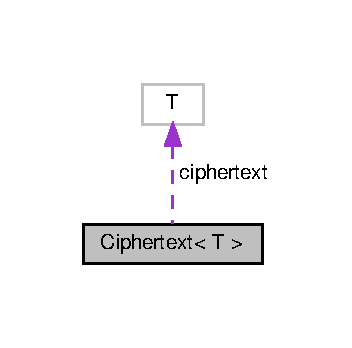
\includegraphics[width=169pt]{classCiphertext__coll__graph}
\end{center}
\end{figure}
\subsection*{Public Member Functions}
\begin{DoxyCompactItemize}
\item 
\hyperlink{classCiphertext_a658bbd14ee1a3683309878e54b575c8f}{Ciphertext} ()
\item 
\hyperlink{classCiphertext_ab04b602d489978f0e511d797b8a8157d}{Ciphertext} (T \&\hyperlink{classCiphertext_adef9aae9d923eb100b4a1ad58ce495f1}{ciphertext})
\item 
virtual \hyperlink{classCiphertext_ab8a4e685883bcc8fbabde6d3c3cb5fd5}{$\sim$\+Ciphertext} ()
\item 
T \hyperlink{classCiphertext_a42d2210e9b019ce36a401ad9a97d03ac}{get\+\_\+ciphertext} ()
\item 
void \hyperlink{classCiphertext_a8ea04527ee2a98ef214edfd8bd0156f8}{set\+\_\+ciphertext} (T \&\hyperlink{classCiphertext_adef9aae9d923eb100b4a1ad58ce495f1}{ciphertext})
\end{DoxyCompactItemize}
\subsection*{Protected Attributes}
\begin{DoxyCompactItemize}
\item 
T \hyperlink{classCiphertext_adef9aae9d923eb100b4a1ad58ce495f1}{ciphertext}
\end{DoxyCompactItemize}


\subsection{Constructor \& Destructor Documentation}
\mbox{\Hypertarget{classCiphertext_a658bbd14ee1a3683309878e54b575c8f}\label{classCiphertext_a658bbd14ee1a3683309878e54b575c8f}} 
\index{Ciphertext@{Ciphertext}!Ciphertext@{Ciphertext}}
\index{Ciphertext@{Ciphertext}!Ciphertext@{Ciphertext}}
\subsubsection{\texorpdfstring{Ciphertext()}{Ciphertext()}\hspace{0.1cm}{\footnotesize\ttfamily [1/2]}}
{\footnotesize\ttfamily template$<$typename T$>$ \\
\hyperlink{classCiphertext}{Ciphertext}$<$ T $>$\+::\hyperlink{classCiphertext}{Ciphertext} (\begin{DoxyParamCaption}{ }\end{DoxyParamCaption})\hspace{0.3cm}{\ttfamily [inline]}}

Default contstructor \mbox{\Hypertarget{classCiphertext_ab04b602d489978f0e511d797b8a8157d}\label{classCiphertext_ab04b602d489978f0e511d797b8a8157d}} 
\index{Ciphertext@{Ciphertext}!Ciphertext@{Ciphertext}}
\index{Ciphertext@{Ciphertext}!Ciphertext@{Ciphertext}}
\subsubsection{\texorpdfstring{Ciphertext()}{Ciphertext()}\hspace{0.1cm}{\footnotesize\ttfamily [2/2]}}
{\footnotesize\ttfamily template$<$typename T$>$ \\
\hyperlink{classCiphertext}{Ciphertext}$<$ T $>$\+::\hyperlink{classCiphertext}{Ciphertext} (\begin{DoxyParamCaption}\item[{T \&}]{ciphertext }\end{DoxyParamCaption})\hspace{0.3cm}{\ttfamily [inline]}}

Initialise ciphertext with the value supplied 
\begin{DoxyParams}{Parameters}
{\em ciphertext} & A ciphertext value \\
\hline
\end{DoxyParams}
\mbox{\Hypertarget{classCiphertext_ab8a4e685883bcc8fbabde6d3c3cb5fd5}\label{classCiphertext_ab8a4e685883bcc8fbabde6d3c3cb5fd5}} 
\index{Ciphertext@{Ciphertext}!````~Ciphertext@{$\sim$\+Ciphertext}}
\index{````~Ciphertext@{$\sim$\+Ciphertext}!Ciphertext@{Ciphertext}}
\subsubsection{\texorpdfstring{$\sim$\+Ciphertext()}{~Ciphertext()}}
{\footnotesize\ttfamily template$<$typename T$>$ \\
virtual \hyperlink{classCiphertext}{Ciphertext}$<$ T $>$\+::$\sim$\hyperlink{classCiphertext}{Ciphertext} (\begin{DoxyParamCaption}{ }\end{DoxyParamCaption})\hspace{0.3cm}{\ttfamily [inline]}, {\ttfamily [virtual]}}

Default destructor 

\subsection{Member Function Documentation}
\mbox{\Hypertarget{classCiphertext_a42d2210e9b019ce36a401ad9a97d03ac}\label{classCiphertext_a42d2210e9b019ce36a401ad9a97d03ac}} 
\index{Ciphertext@{Ciphertext}!get\+\_\+ciphertext@{get\+\_\+ciphertext}}
\index{get\+\_\+ciphertext@{get\+\_\+ciphertext}!Ciphertext@{Ciphertext}}
\subsubsection{\texorpdfstring{get\+\_\+ciphertext()}{get\_ciphertext()}}
{\footnotesize\ttfamily template$<$typename T$>$ \\
T \hyperlink{classCiphertext}{Ciphertext}$<$ T $>$\+::get\+\_\+ciphertext (\begin{DoxyParamCaption}{ }\end{DoxyParamCaption})\hspace{0.3cm}{\ttfamily [inline]}}

Accessor to return the ciphertext member \begin{DoxyReturn}{Returns}
\hyperlink{classCiphertext}{Ciphertext} value 
\end{DoxyReturn}
\mbox{\Hypertarget{classCiphertext_a8ea04527ee2a98ef214edfd8bd0156f8}\label{classCiphertext_a8ea04527ee2a98ef214edfd8bd0156f8}} 
\index{Ciphertext@{Ciphertext}!set\+\_\+ciphertext@{set\+\_\+ciphertext}}
\index{set\+\_\+ciphertext@{set\+\_\+ciphertext}!Ciphertext@{Ciphertext}}
\subsubsection{\texorpdfstring{set\+\_\+ciphertext()}{set\_ciphertext()}}
{\footnotesize\ttfamily template$<$typename T$>$ \\
void \hyperlink{classCiphertext}{Ciphertext}$<$ T $>$\+::set\+\_\+ciphertext (\begin{DoxyParamCaption}\item[{T \&}]{ciphertext }\end{DoxyParamCaption})\hspace{0.3cm}{\ttfamily [inline]}}

Accessor to set the ciphertext member 
\begin{DoxyParams}{Parameters}
{\em ciphertext} & \hyperlink{classCiphertext}{Ciphertext} value \\
\hline
\end{DoxyParams}


\subsection{Member Data Documentation}
\mbox{\Hypertarget{classCiphertext_adef9aae9d923eb100b4a1ad58ce495f1}\label{classCiphertext_adef9aae9d923eb100b4a1ad58ce495f1}} 
\index{Ciphertext@{Ciphertext}!ciphertext@{ciphertext}}
\index{ciphertext@{ciphertext}!Ciphertext@{Ciphertext}}
\subsubsection{\texorpdfstring{ciphertext}{ciphertext}}
{\footnotesize\ttfamily template$<$typename T$>$ \\
T \hyperlink{classCiphertext}{Ciphertext}$<$ T $>$\+::ciphertext\hspace{0.3cm}{\ttfamily [protected]}}

The ciphertext value encapsulated by this object 

The documentation for this class was generated from the following file\+:\begin{DoxyCompactItemize}
\item 
include/\hyperlink{Ciphertext_8hpp}{Ciphertext.\+hpp}\end{DoxyCompactItemize}

\hypertarget{classDETCiphertext}{}\section{D\+E\+T\+Ciphertext Class Reference}
\label{classDETCiphertext}\index{D\+E\+T\+Ciphertext@{D\+E\+T\+Ciphertext}}


{\ttfamily \#include $<$D\+E\+T\+Ciphertext.\+h$>$}



Inheritance diagram for D\+E\+T\+Ciphertext\+:
\nopagebreak
\begin{figure}[H]
\begin{center}
\leavevmode
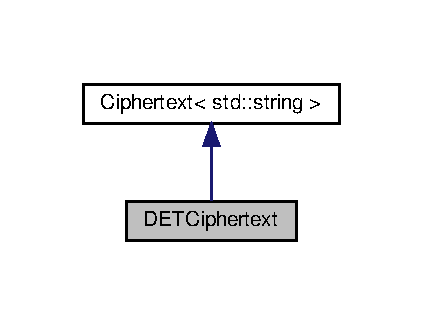
\includegraphics[width=203pt]{classDETCiphertext__inherit__graph}
\end{center}
\end{figure}


Collaboration diagram for D\+E\+T\+Ciphertext\+:
\nopagebreak
\begin{figure}[H]
\begin{center}
\leavevmode
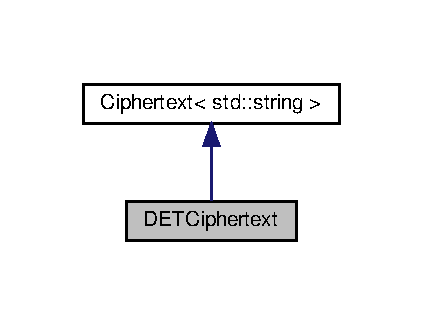
\includegraphics[width=203pt]{classDETCiphertext__coll__graph}
\end{center}
\end{figure}
\subsection*{Public Member Functions}
\begin{DoxyCompactItemize}
\item 
\hyperlink{classDETCiphertext_abf102b1ca2a4dc34ee71e4ed92df3977}{D\+E\+T\+Ciphertext} ()
\item 
\hyperlink{classDETCiphertext_a92b651e8e700ef303b0cb1d6a1995ba4}{D\+E\+T\+Ciphertext} (std\+::string \&\hyperlink{classCiphertext_adef9aae9d923eb100b4a1ad58ce495f1}{ciphertext})
\item 
virtual \hyperlink{classDETCiphertext_ae9a37b2c41fc81e8b8948d3bcf057cd6}{$\sim$\+D\+E\+T\+Ciphertext} ()
\end{DoxyCompactItemize}
\subsection*{Private Member Functions}
\begin{DoxyCompactItemize}
\item 
{\footnotesize template$<$class Archive $>$ }\\void \hyperlink{classDETCiphertext_a1c1a7050c492627da2b277d9064635e6}{serialize} (Archive \&ar, const unsigned int version)
\end{DoxyCompactItemize}
\subsection*{Friends}
\begin{DoxyCompactItemize}
\item 
class \hyperlink{classDETCiphertext_ac98d07dd8f7b70e16ccb9a01abf56b9c}{boost\+::serialization\+::access}
\item 
bool \hyperlink{classDETCiphertext_a5f7e97804478b1b2badc92d540797b73}{operator==} (\hyperlink{classDETCiphertext}{D\+E\+T\+Ciphertext} \&a, \hyperlink{classDETCiphertext}{D\+E\+T\+Ciphertext} \&b)
\end{DoxyCompactItemize}
\subsection*{Additional Inherited Members}


\subsection{Constructor \& Destructor Documentation}
\mbox{\Hypertarget{classDETCiphertext_abf102b1ca2a4dc34ee71e4ed92df3977}\label{classDETCiphertext_abf102b1ca2a4dc34ee71e4ed92df3977}} 
\index{D\+E\+T\+Ciphertext@{D\+E\+T\+Ciphertext}!D\+E\+T\+Ciphertext@{D\+E\+T\+Ciphertext}}
\index{D\+E\+T\+Ciphertext@{D\+E\+T\+Ciphertext}!D\+E\+T\+Ciphertext@{D\+E\+T\+Ciphertext}}
\subsubsection{\texorpdfstring{D\+E\+T\+Ciphertext()}{DETCiphertext()}\hspace{0.1cm}{\footnotesize\ttfamily [1/2]}}
{\footnotesize\ttfamily D\+E\+T\+Ciphertext\+::\+D\+E\+T\+Ciphertext (\begin{DoxyParamCaption}{ }\end{DoxyParamCaption})}

Default constructor \mbox{\Hypertarget{classDETCiphertext_a92b651e8e700ef303b0cb1d6a1995ba4}\label{classDETCiphertext_a92b651e8e700ef303b0cb1d6a1995ba4}} 
\index{D\+E\+T\+Ciphertext@{D\+E\+T\+Ciphertext}!D\+E\+T\+Ciphertext@{D\+E\+T\+Ciphertext}}
\index{D\+E\+T\+Ciphertext@{D\+E\+T\+Ciphertext}!D\+E\+T\+Ciphertext@{D\+E\+T\+Ciphertext}}
\subsubsection{\texorpdfstring{D\+E\+T\+Ciphertext()}{DETCiphertext()}\hspace{0.1cm}{\footnotesize\ttfamily [2/2]}}
{\footnotesize\ttfamily D\+E\+T\+Ciphertext\+::\+D\+E\+T\+Ciphertext (\begin{DoxyParamCaption}\item[{std\+::string \&}]{ciphertext }\end{DoxyParamCaption})}

Initialise {\ttfamily ciphertext} with the supplied byte string 
\begin{DoxyParams}{Parameters}
{\em ciphertext} & A byte string \\
\hline
\end{DoxyParams}
\mbox{\Hypertarget{classDETCiphertext_ae9a37b2c41fc81e8b8948d3bcf057cd6}\label{classDETCiphertext_ae9a37b2c41fc81e8b8948d3bcf057cd6}} 
\index{D\+E\+T\+Ciphertext@{D\+E\+T\+Ciphertext}!````~D\+E\+T\+Ciphertext@{$\sim$\+D\+E\+T\+Ciphertext}}
\index{````~D\+E\+T\+Ciphertext@{$\sim$\+D\+E\+T\+Ciphertext}!D\+E\+T\+Ciphertext@{D\+E\+T\+Ciphertext}}
\subsubsection{\texorpdfstring{$\sim$\+D\+E\+T\+Ciphertext()}{~DETCiphertext()}}
{\footnotesize\ttfamily D\+E\+T\+Ciphertext\+::$\sim$\+D\+E\+T\+Ciphertext (\begin{DoxyParamCaption}{ }\end{DoxyParamCaption})\hspace{0.3cm}{\ttfamily [virtual]}}

Default destructor 

\subsection{Member Function Documentation}
\mbox{\Hypertarget{classDETCiphertext_a1c1a7050c492627da2b277d9064635e6}\label{classDETCiphertext_a1c1a7050c492627da2b277d9064635e6}} 
\index{D\+E\+T\+Ciphertext@{D\+E\+T\+Ciphertext}!serialize@{serialize}}
\index{serialize@{serialize}!D\+E\+T\+Ciphertext@{D\+E\+T\+Ciphertext}}
\subsubsection{\texorpdfstring{serialize()}{serialize()}}
{\footnotesize\ttfamily template$<$class Archive $>$ \\
void D\+E\+T\+Ciphertext\+::serialize (\begin{DoxyParamCaption}\item[{Archive \&}]{ar,  }\item[{const unsigned int}]{version }\end{DoxyParamCaption})\hspace{0.3cm}{\ttfamily [inline]}, {\ttfamily [private]}}



\subsection{Friends And Related Function Documentation}
\mbox{\Hypertarget{classDETCiphertext_ac98d07dd8f7b70e16ccb9a01abf56b9c}\label{classDETCiphertext_ac98d07dd8f7b70e16ccb9a01abf56b9c}} 
\index{D\+E\+T\+Ciphertext@{D\+E\+T\+Ciphertext}!boost\+::serialization\+::access@{boost\+::serialization\+::access}}
\index{boost\+::serialization\+::access@{boost\+::serialization\+::access}!D\+E\+T\+Ciphertext@{D\+E\+T\+Ciphertext}}
\subsubsection{\texorpdfstring{boost\+::serialization\+::access}{boost::serialization::access}}
{\footnotesize\ttfamily friend class boost\+::serialization\+::access\hspace{0.3cm}{\ttfamily [friend]}}

\mbox{\Hypertarget{classDETCiphertext_a5f7e97804478b1b2badc92d540797b73}\label{classDETCiphertext_a5f7e97804478b1b2badc92d540797b73}} 
\index{D\+E\+T\+Ciphertext@{D\+E\+T\+Ciphertext}!operator==@{operator==}}
\index{operator==@{operator==}!D\+E\+T\+Ciphertext@{D\+E\+T\+Ciphertext}}
\subsubsection{\texorpdfstring{operator==}{operator==}}
{\footnotesize\ttfamily bool operator== (\begin{DoxyParamCaption}\item[{\hyperlink{classDETCiphertext}{D\+E\+T\+Ciphertext} \&}]{a,  }\item[{\hyperlink{classDETCiphertext}{D\+E\+T\+Ciphertext} \&}]{b }\end{DoxyParamCaption})\hspace{0.3cm}{\ttfamily [friend]}}

Return {\ttfamily a.\+ciphertext} = {\ttfamily b.\+ciphertext} 
\begin{DoxyParams}{Parameters}
{\em a} & A {\ttfamily \hyperlink{classDETCiphertext}{D\+E\+T\+Ciphertext}} object \\
\hline
{\em b} & A {\ttfamily \hyperlink{classDETCiphertext}{D\+E\+T\+Ciphertext}} object \\
\hline
\end{DoxyParams}
\begin{DoxyReturn}{Returns}
{\ttfamily true} or {\ttfamily false} 
\end{DoxyReturn}


The documentation for this class was generated from the following files\+:\begin{DoxyCompactItemize}
\item 
include/\hyperlink{DETCiphertext_8h}{D\+E\+T\+Ciphertext.\+h}\item 
src/\hyperlink{DETCiphertext_8cpp}{D\+E\+T\+Ciphertext.\+cpp}\end{DoxyCompactItemize}

\hypertarget{classHE1Array}{}\section{H\+E1\+Array Class Reference}
\label{classHE1Array}\index{H\+E1\+Array@{H\+E1\+Array}}


{\ttfamily \#include $<$H\+E1\+Array.\+h$>$}



Inheritance diagram for H\+E1\+Array\+:
\nopagebreak
\begin{figure}[H]
\begin{center}
\leavevmode
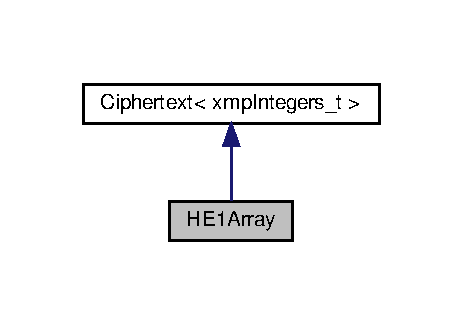
\includegraphics[width=222pt]{classHE1Array__inherit__graph}
\end{center}
\end{figure}


Collaboration diagram for H\+E1\+Array\+:
\nopagebreak
\begin{figure}[H]
\begin{center}
\leavevmode
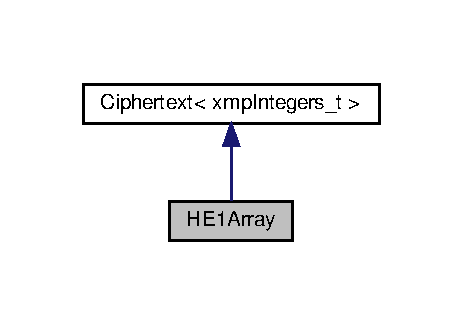
\includegraphics[width=222pt]{classHE1Array__coll__graph}
\end{center}
\end{figure}
\subsection*{Public Member Functions}
\begin{DoxyCompactItemize}
\item 
\hyperlink{classHE1Array_a99381587cd348b91f90a94fe5b25a3a3}{H\+E1\+Array} (unsigned int \hyperlink{classHE1Array_a486ac51b636d5434c6d456a0b470ab1e}{count})
\item 
\hyperlink{classHE1Array_a8c961c822603135c972b7fefc555f560}{H\+E1\+Array} (int value, unsigned int \hyperlink{classHE1Array_a486ac51b636d5434c6d456a0b470ab1e}{count})
\item 
\hyperlink{classHE1Array_af000ef4656e6b1136b9aaec07e683ad0}{H\+E1\+Array} (N\+T\+L\+::\+ZZ \&value)
\item 
\hyperlink{classHE1Array_aa2bc58501546488b6d05b7f14b2f8ec3}{H\+E1\+Array} (xmp\+Integers\+\_\+t \hyperlink{classCiphertext_adef9aae9d923eb100b4a1ad58ce495f1}{ciphertext}, unsigned int \hyperlink{classHE1Array_a486ac51b636d5434c6d456a0b470ab1e}{count})
\item 
\hyperlink{classHE1Array_ab07215fb33d5e7c2422ef7201752759b}{H\+E1\+Array} (\hyperlink{HE1Array_8h_a19036394f9c80a08fc846c96f668711c}{word} $\ast$inputs, unsigned int \hyperlink{classHE1Array_a486ac51b636d5434c6d456a0b470ab1e}{count})
\item 
\hyperlink{classHE1Array_a83a31561044fe24c711526bb2e137de7}{H\+E1\+Array} (N\+T\+L\+::vec\+\_\+\+ZZ \&v)
\item 
virtual \hyperlink{classHE1Array_a9aa03bcb90dfa12ed1666ef9b7825bcf}{$\sim$\+H\+E1\+Array} ()
\item 
void \hyperlink{classHE1Array_a1fb765c051988639c3d4f33b6c166035}{set\+\_\+zero} ()
\item 
unsigned int \hyperlink{classHE1Array_a87b0a1931df4e220fe3c9ae92ba2ce64}{get\+\_\+count} ()
\item 
N\+T\+L\+::vec\+\_\+\+ZZ \hyperlink{classHE1Array_a43de83bb8ed2cf9063e60acccd2031e8}{to\+\_\+\+Z\+Z\+\_\+vector} ()
\item 
std\+::vector$<$ \hyperlink{HE1Array_8h_a19036394f9c80a08fc846c96f668711c}{word} $>$ \hyperlink{classHE1Array_af689c0f38383fb15efcff72563a9187b}{to\+\_\+host\+\_\+array} ()
\item 
\hyperlink{classHE1Array}{H\+E1\+Array} \& \hyperlink{classHE1Array_ab2a255ca11e099aa6e331133302edc10}{operator$\ast$=} (\hyperlink{classHE1Array}{H\+E1\+Array} \&o)
\item 
\hyperlink{classHE1Array}{H\+E1\+Array} \& \hyperlink{classHE1Array_a3bf3040c4a13cf3b83730dcc8d01b352}{operator+=} (\hyperlink{classHE1Array}{H\+E1\+Array} \&o)
\end{DoxyCompactItemize}
\subsection*{Static Public Member Functions}
\begin{DoxyCompactItemize}
\item 
static void \hyperlink{classHE1Array_ab07c3a11d23c4115ef3495482fb65fb0}{create\+\_\+device\+\_\+handle} ()
\item 
static void \hyperlink{classHE1Array_a38ce380d3cdb0dd9e59c0515af87493c}{delete\+\_\+device\+\_\+handle} ()
\item 
static void \hyperlink{classHE1Array_aa57bea5fd5ce8288a868cacc9ec69c90}{create\+\_\+device\+\_\+modulus} (N\+T\+L\+::\+ZZ \&\hyperlink{classHE1Array_a164afa9080888fad5d805a98021d9c57}{modulus})
\item 
static void \hyperlink{classHE1Array_a11536c5066ce8bddb7e8ddf3e9de6146}{delete\+\_\+device\+\_\+modulus} ()
\end{DoxyCompactItemize}
\subsection*{Static Private Member Functions}
\begin{DoxyCompactItemize}
\item 
static std\+::vector$<$ \hyperlink{HE1Array_8h_a19036394f9c80a08fc846c96f668711c}{word} $>$ \hyperlink{classHE1Array_a60718a561d39e7036c32abcf92c5c9c1}{Z\+Z\+\_\+to\+\_\+word\+\_\+array} (N\+T\+L\+::\+ZZ \&z, int num\+Words)
\end{DoxyCompactItemize}
\subsection*{Private Attributes}
\begin{DoxyCompactItemize}
\item 
unsigned int \hyperlink{classHE1Array_a486ac51b636d5434c6d456a0b470ab1e}{count}
\end{DoxyCompactItemize}
\subsection*{Static Private Attributes}
\begin{DoxyCompactItemize}
\item 
static xmp\+Integers\+\_\+t \hyperlink{classHE1Array_a164afa9080888fad5d805a98021d9c57}{modulus}
\item 
static xmp\+Handle\+\_\+t \hyperlink{classHE1Array_a6f4fd4ae4280b6ac4abe146f80a0ade4}{handle}
\item 
static unsigned int \hyperlink{classHE1Array_a552ef796b7fa4c00e142acdc78852a89}{max\+Precision}
\item 
static unsigned int \hyperlink{classHE1Array_acfcbb207535ce6e489b986e36080c784}{max\+Words}
\end{DoxyCompactItemize}
\subsection*{Friends}
\begin{DoxyCompactItemize}
\item 
\hyperlink{classHE1Array}{H\+E1\+Array} \hyperlink{classHE1Array_a9af458afd1fae2464406a71868d411d9}{operator$\ast$} (\hyperlink{classHE1Array}{H\+E1\+Array} \&a, \hyperlink{classHE1Array}{H\+E1\+Array} \&b)
\item 
\hyperlink{classHE1Array}{H\+E1\+Array} \hyperlink{classHE1Array_aaa51e336d1bca00b78a39445cc9525ec}{operator+} (\hyperlink{classHE1Array}{H\+E1\+Array} \&a, \hyperlink{classHE1Array}{H\+E1\+Array} \&b)
\end{DoxyCompactItemize}
\subsection*{Additional Inherited Members}


\subsection{Constructor \& Destructor Documentation}
\mbox{\Hypertarget{classHE1Array_a99381587cd348b91f90a94fe5b25a3a3}\label{classHE1Array_a99381587cd348b91f90a94fe5b25a3a3}} 
\index{H\+E1\+Array@{H\+E1\+Array}!H\+E1\+Array@{H\+E1\+Array}}
\index{H\+E1\+Array@{H\+E1\+Array}!H\+E1\+Array@{H\+E1\+Array}}
\subsubsection{\texorpdfstring{H\+E1\+Array()}{HE1Array()}\hspace{0.1cm}{\footnotesize\ttfamily [1/6]}}
{\footnotesize\ttfamily H\+E1\+Array\+::\+H\+E1\+Array (\begin{DoxyParamCaption}\item[{unsigned int}]{count }\end{DoxyParamCaption})}

Default constructor. It allocates memory for a device array of {\itshape count} multiprecision integers 
\begin{DoxyParams}{Parameters}
{\em count} & The number of multiprecision integers in the device array \\
\hline
\end{DoxyParams}
\mbox{\Hypertarget{classHE1Array_a8c961c822603135c972b7fefc555f560}\label{classHE1Array_a8c961c822603135c972b7fefc555f560}} 
\index{H\+E1\+Array@{H\+E1\+Array}!H\+E1\+Array@{H\+E1\+Array}}
\index{H\+E1\+Array@{H\+E1\+Array}!H\+E1\+Array@{H\+E1\+Array}}
\subsubsection{\texorpdfstring{H\+E1\+Array()}{HE1Array()}\hspace{0.1cm}{\footnotesize\ttfamily [2/6]}}
{\footnotesize\ttfamily H\+E1\+Array\+::\+H\+E1\+Array (\begin{DoxyParamCaption}\item[{int}]{value,  }\item[{unsigned int}]{count }\end{DoxyParamCaption})}

This constructor allocates memory for a device array of {\itshape count} multiprecision integers and initialises each integer to {\itshape value} 
\begin{DoxyParams}{Parameters}
{\em value} & The initial value of each integer. \\
\hline
{\em count} & The number of multiprecision integers in the device array \\
\hline
\end{DoxyParams}
\mbox{\Hypertarget{classHE1Array_af000ef4656e6b1136b9aaec07e683ad0}\label{classHE1Array_af000ef4656e6b1136b9aaec07e683ad0}} 
\index{H\+E1\+Array@{H\+E1\+Array}!H\+E1\+Array@{H\+E1\+Array}}
\index{H\+E1\+Array@{H\+E1\+Array}!H\+E1\+Array@{H\+E1\+Array}}
\subsubsection{\texorpdfstring{H\+E1\+Array()}{HE1Array()}\hspace{0.1cm}{\footnotesize\ttfamily [3/6]}}
{\footnotesize\ttfamily H\+E1\+Array\+::\+H\+E1\+Array (\begin{DoxyParamCaption}\item[{N\+T\+L\+::\+ZZ \&}]{value }\end{DoxyParamCaption})}

This constructor allocates memory for a single multiprecision integer and initialises it to {\itshape value}, an N\+TL multiprecision integer 
\begin{DoxyParams}{Parameters}
{\em value} & Intial value of integer \\
\hline
\end{DoxyParams}
\mbox{\Hypertarget{classHE1Array_aa2bc58501546488b6d05b7f14b2f8ec3}\label{classHE1Array_aa2bc58501546488b6d05b7f14b2f8ec3}} 
\index{H\+E1\+Array@{H\+E1\+Array}!H\+E1\+Array@{H\+E1\+Array}}
\index{H\+E1\+Array@{H\+E1\+Array}!H\+E1\+Array@{H\+E1\+Array}}
\subsubsection{\texorpdfstring{H\+E1\+Array()}{HE1Array()}\hspace{0.1cm}{\footnotesize\ttfamily [4/6]}}
{\footnotesize\ttfamily H\+E1\+Array\+::\+H\+E1\+Array (\begin{DoxyParamCaption}\item[{xmp\+Integers\+\_\+t}]{ciphertext,  }\item[{unsigned int}]{count }\end{DoxyParamCaption})}

This constructor copies the {\ttfamily xmp\+Integers\+\_\+t} object into the {\ttfamily ciphertext} member. 
\begin{DoxyParams}{Parameters}
{\em ciphertext} & {\ttfamily xmp\+Integers\+\_\+t} object \\
\hline
{\em count} & Number of integers in {\ttfamily xmp\+Integers\+\_\+t} object \\
\hline
\end{DoxyParams}
\mbox{\Hypertarget{classHE1Array_ab07215fb33d5e7c2422ef7201752759b}\label{classHE1Array_ab07215fb33d5e7c2422ef7201752759b}} 
\index{H\+E1\+Array@{H\+E1\+Array}!H\+E1\+Array@{H\+E1\+Array}}
\index{H\+E1\+Array@{H\+E1\+Array}!H\+E1\+Array@{H\+E1\+Array}}
\subsubsection{\texorpdfstring{H\+E1\+Array()}{HE1Array()}\hspace{0.1cm}{\footnotesize\ttfamily [5/6]}}
{\footnotesize\ttfamily H\+E1\+Array\+::\+H\+E1\+Array (\begin{DoxyParamCaption}\item[{\hyperlink{HE1Array_8h_a19036394f9c80a08fc846c96f668711c}{word} $\ast$}]{inputs,  }\item[{unsigned int}]{count }\end{DoxyParamCaption})}

Initialise {\ttfamily xmp\+Integers\+\_\+t} member by loading an array of words (word size is 4 bytes) 
\begin{DoxyParams}{Parameters}
{\em inputs} & Word array \\
\hline
{\em count} & Number of integers in array \\
\hline
\end{DoxyParams}
\mbox{\Hypertarget{classHE1Array_a83a31561044fe24c711526bb2e137de7}\label{classHE1Array_a83a31561044fe24c711526bb2e137de7}} 
\index{H\+E1\+Array@{H\+E1\+Array}!H\+E1\+Array@{H\+E1\+Array}}
\index{H\+E1\+Array@{H\+E1\+Array}!H\+E1\+Array@{H\+E1\+Array}}
\subsubsection{\texorpdfstring{H\+E1\+Array()}{HE1Array()}\hspace{0.1cm}{\footnotesize\ttfamily [6/6]}}
{\footnotesize\ttfamily H\+E1\+Array\+::\+H\+E1\+Array (\begin{DoxyParamCaption}\item[{N\+T\+L\+::vec\+\_\+\+ZZ \&}]{v }\end{DoxyParamCaption})}

Intialise {\ttfamily xmp\+Integers\+\_\+t} member using a vector of N\+TL multiprecision integers 
\begin{DoxyParams}{Parameters}
{\em v} & A vector of N\+TL multiprecision integers \\
\hline
\end{DoxyParams}
\mbox{\Hypertarget{classHE1Array_a9aa03bcb90dfa12ed1666ef9b7825bcf}\label{classHE1Array_a9aa03bcb90dfa12ed1666ef9b7825bcf}} 
\index{H\+E1\+Array@{H\+E1\+Array}!````~H\+E1\+Array@{$\sim$\+H\+E1\+Array}}
\index{````~H\+E1\+Array@{$\sim$\+H\+E1\+Array}!H\+E1\+Array@{H\+E1\+Array}}
\subsubsection{\texorpdfstring{$\sim$\+H\+E1\+Array()}{~HE1Array()}}
{\footnotesize\ttfamily H\+E1\+Array\+::$\sim$\+H\+E1\+Array (\begin{DoxyParamCaption}{ }\end{DoxyParamCaption})\hspace{0.3cm}{\ttfamily [virtual]}}

Default virtual destructor. It frees the memory on the device allocated to {\ttfamily xmp\+Integers\+\_\+t} {\ttfamily ciphertext} member. 

\subsection{Member Function Documentation}
\mbox{\Hypertarget{classHE1Array_ab07c3a11d23c4115ef3495482fb65fb0}\label{classHE1Array_ab07c3a11d23c4115ef3495482fb65fb0}} 
\index{H\+E1\+Array@{H\+E1\+Array}!create\+\_\+device\+\_\+handle@{create\+\_\+device\+\_\+handle}}
\index{create\+\_\+device\+\_\+handle@{create\+\_\+device\+\_\+handle}!H\+E1\+Array@{H\+E1\+Array}}
\subsubsection{\texorpdfstring{create\+\_\+device\+\_\+handle()}{create\_device\_handle()}}
{\footnotesize\ttfamily void H\+E1\+Array\+::create\+\_\+device\+\_\+handle (\begin{DoxyParamCaption}{ }\end{DoxyParamCaption})\hspace{0.3cm}{\ttfamily [static]}}

A static class method to create an X\+MP device context handle. \mbox{\Hypertarget{classHE1Array_aa57bea5fd5ce8288a868cacc9ec69c90}\label{classHE1Array_aa57bea5fd5ce8288a868cacc9ec69c90}} 
\index{H\+E1\+Array@{H\+E1\+Array}!create\+\_\+device\+\_\+modulus@{create\+\_\+device\+\_\+modulus}}
\index{create\+\_\+device\+\_\+modulus@{create\+\_\+device\+\_\+modulus}!H\+E1\+Array@{H\+E1\+Array}}
\subsubsection{\texorpdfstring{create\+\_\+device\+\_\+modulus()}{create\_device\_modulus()}}
{\footnotesize\ttfamily void H\+E1\+Array\+::create\+\_\+device\+\_\+modulus (\begin{DoxyParamCaption}\item[{N\+T\+L\+::\+ZZ \&}]{mod }\end{DoxyParamCaption})\hspace{0.3cm}{\ttfamily [static]}}

Creates an {\ttfamily xmp\+Integers\+\_\+t} on the device to store the modulus for arithmetic and assigns {\ttfamily mod} to it. {\ttfamily max\+Precision} and {\ttfamily max\+Words} are set to the number of bits and words required to store {\ttfamily mod}. 
\begin{DoxyParams}{Parameters}
{\em mod} & An N\+TL multiprecision integer containing the modulus \\
\hline
\end{DoxyParams}
\mbox{\Hypertarget{classHE1Array_a38ce380d3cdb0dd9e59c0515af87493c}\label{classHE1Array_a38ce380d3cdb0dd9e59c0515af87493c}} 
\index{H\+E1\+Array@{H\+E1\+Array}!delete\+\_\+device\+\_\+handle@{delete\+\_\+device\+\_\+handle}}
\index{delete\+\_\+device\+\_\+handle@{delete\+\_\+device\+\_\+handle}!H\+E1\+Array@{H\+E1\+Array}}
\subsubsection{\texorpdfstring{delete\+\_\+device\+\_\+handle()}{delete\_device\_handle()}}
{\footnotesize\ttfamily void H\+E1\+Array\+::delete\+\_\+device\+\_\+handle (\begin{DoxyParamCaption}{ }\end{DoxyParamCaption})\hspace{0.3cm}{\ttfamily [static]}}

A static class method to destroy an existing X\+MP device context handle. \mbox{\Hypertarget{classHE1Array_a11536c5066ce8bddb7e8ddf3e9de6146}\label{classHE1Array_a11536c5066ce8bddb7e8ddf3e9de6146}} 
\index{H\+E1\+Array@{H\+E1\+Array}!delete\+\_\+device\+\_\+modulus@{delete\+\_\+device\+\_\+modulus}}
\index{delete\+\_\+device\+\_\+modulus@{delete\+\_\+device\+\_\+modulus}!H\+E1\+Array@{H\+E1\+Array}}
\subsubsection{\texorpdfstring{delete\+\_\+device\+\_\+modulus()}{delete\_device\_modulus()}}
{\footnotesize\ttfamily void H\+E1\+Array\+::delete\+\_\+device\+\_\+modulus (\begin{DoxyParamCaption}{ }\end{DoxyParamCaption})\hspace{0.3cm}{\ttfamily [static]}}

Destroys the {\ttfamily xmp\+Integers\+\_\+t} containing the modulus \mbox{\Hypertarget{classHE1Array_a87b0a1931df4e220fe3c9ae92ba2ce64}\label{classHE1Array_a87b0a1931df4e220fe3c9ae92ba2ce64}} 
\index{H\+E1\+Array@{H\+E1\+Array}!get\+\_\+count@{get\+\_\+count}}
\index{get\+\_\+count@{get\+\_\+count}!H\+E1\+Array@{H\+E1\+Array}}
\subsubsection{\texorpdfstring{get\+\_\+count()}{get\_count()}}
{\footnotesize\ttfamily unsigned int H\+E1\+Array\+::get\+\_\+count (\begin{DoxyParamCaption}{ }\end{DoxyParamCaption})}

Accessor to get the number of integers stored in {\ttfamily ciphertext} \begin{DoxyReturn}{Returns}
The number of integers stored in {\ttfamily ciphertext} 
\end{DoxyReturn}
\mbox{\Hypertarget{classHE1Array_ab2a255ca11e099aa6e331133302edc10}\label{classHE1Array_ab2a255ca11e099aa6e331133302edc10}} 
\index{H\+E1\+Array@{H\+E1\+Array}!operator$\ast$=@{operator$\ast$=}}
\index{operator$\ast$=@{operator$\ast$=}!H\+E1\+Array@{H\+E1\+Array}}
\subsubsection{\texorpdfstring{operator$\ast$=()}{operator*=()}}
{\footnotesize\ttfamily \hyperlink{classHE1Array}{H\+E1\+Array} \& H\+E1\+Array\+::operator$\ast$= (\begin{DoxyParamCaption}\item[{\hyperlink{classHE1Array}{H\+E1\+Array} \&}]{o }\end{DoxyParamCaption})}

Performs modular multiplication of the integers in {\ttfamily ciphertext} with those in the {\ttfamily ciphertext} member of {\ttfamily o}. 
\begin{DoxyParams}{Parameters}
{\em o} & Another {\ttfamily \hyperlink{classHE1Array}{H\+E1\+Array}} object \\
\hline
\end{DoxyParams}
\begin{DoxyReturn}{Returns}
{\ttfamily this} object 
\end{DoxyReturn}
\mbox{\Hypertarget{classHE1Array_a3bf3040c4a13cf3b83730dcc8d01b352}\label{classHE1Array_a3bf3040c4a13cf3b83730dcc8d01b352}} 
\index{H\+E1\+Array@{H\+E1\+Array}!operator+=@{operator+=}}
\index{operator+=@{operator+=}!H\+E1\+Array@{H\+E1\+Array}}
\subsubsection{\texorpdfstring{operator+=()}{operator+=()}}
{\footnotesize\ttfamily \hyperlink{classHE1Array}{H\+E1\+Array} \& H\+E1\+Array\+::operator+= (\begin{DoxyParamCaption}\item[{\hyperlink{classHE1Array}{H\+E1\+Array} \&}]{o }\end{DoxyParamCaption})}

Performs modular addition of the integers in {\ttfamily ciphertext} with those in the {\ttfamily ciphertext} member of {\ttfamily o}. 
\begin{DoxyParams}{Parameters}
{\em o} & Another {\ttfamily \hyperlink{classHE1Array}{H\+E1\+Array}} object \\
\hline
\end{DoxyParams}
\begin{DoxyReturn}{Returns}
{\ttfamily this} object 
\end{DoxyReturn}
\mbox{\Hypertarget{classHE1Array_a1fb765c051988639c3d4f33b6c166035}\label{classHE1Array_a1fb765c051988639c3d4f33b6c166035}} 
\index{H\+E1\+Array@{H\+E1\+Array}!set\+\_\+zero@{set\+\_\+zero}}
\index{set\+\_\+zero@{set\+\_\+zero}!H\+E1\+Array@{H\+E1\+Array}}
\subsubsection{\texorpdfstring{set\+\_\+zero()}{set\_zero()}}
{\footnotesize\ttfamily void H\+E1\+Array\+::set\+\_\+zero (\begin{DoxyParamCaption}{ }\end{DoxyParamCaption})}

Set {\ttfamily ciphertext} to an array of zeros \mbox{\Hypertarget{classHE1Array_af689c0f38383fb15efcff72563a9187b}\label{classHE1Array_af689c0f38383fb15efcff72563a9187b}} 
\index{H\+E1\+Array@{H\+E1\+Array}!to\+\_\+host\+\_\+array@{to\+\_\+host\+\_\+array}}
\index{to\+\_\+host\+\_\+array@{to\+\_\+host\+\_\+array}!H\+E1\+Array@{H\+E1\+Array}}
\subsubsection{\texorpdfstring{to\+\_\+host\+\_\+array()}{to\_host\_array()}}
{\footnotesize\ttfamily std\+::vector$<$ \hyperlink{HE1Array_8h_a19036394f9c80a08fc846c96f668711c}{word} $>$ H\+E1\+Array\+::to\+\_\+host\+\_\+array (\begin{DoxyParamCaption}{ }\end{DoxyParamCaption})}

Export the data in {\ttfamily ciphertext} to a host word array \begin{DoxyReturn}{Returns}
An array of words (4 bytes) 
\end{DoxyReturn}
\mbox{\Hypertarget{classHE1Array_a43de83bb8ed2cf9063e60acccd2031e8}\label{classHE1Array_a43de83bb8ed2cf9063e60acccd2031e8}} 
\index{H\+E1\+Array@{H\+E1\+Array}!to\+\_\+\+Z\+Z\+\_\+vector@{to\+\_\+\+Z\+Z\+\_\+vector}}
\index{to\+\_\+\+Z\+Z\+\_\+vector@{to\+\_\+\+Z\+Z\+\_\+vector}!H\+E1\+Array@{H\+E1\+Array}}
\subsubsection{\texorpdfstring{to\+\_\+\+Z\+Z\+\_\+vector()}{to\_ZZ\_vector()}}
{\footnotesize\ttfamily N\+T\+L\+::vec\+\_\+\+ZZ H\+E1\+Array\+::to\+\_\+\+Z\+Z\+\_\+vector (\begin{DoxyParamCaption}{ }\end{DoxyParamCaption})}

Export the data in {\ttfamily ciphertext} to an N\+TL vector of integers \begin{DoxyReturn}{Returns}
N\+TL integer vector 
\end{DoxyReturn}
\mbox{\Hypertarget{classHE1Array_a60718a561d39e7036c32abcf92c5c9c1}\label{classHE1Array_a60718a561d39e7036c32abcf92c5c9c1}} 
\index{H\+E1\+Array@{H\+E1\+Array}!Z\+Z\+\_\+to\+\_\+word\+\_\+array@{Z\+Z\+\_\+to\+\_\+word\+\_\+array}}
\index{Z\+Z\+\_\+to\+\_\+word\+\_\+array@{Z\+Z\+\_\+to\+\_\+word\+\_\+array}!H\+E1\+Array@{H\+E1\+Array}}
\subsubsection{\texorpdfstring{Z\+Z\+\_\+to\+\_\+word\+\_\+array()}{ZZ\_to\_word\_array()}}
{\footnotesize\ttfamily std\+::vector$<$ \hyperlink{HE1Array_8h_a19036394f9c80a08fc846c96f668711c}{word} $>$ H\+E1\+Array\+::\+Z\+Z\+\_\+to\+\_\+word\+\_\+array (\begin{DoxyParamCaption}\item[{N\+T\+L\+::\+ZZ \&}]{z,  }\item[{int}]{num\+Words }\end{DoxyParamCaption})\hspace{0.3cm}{\ttfamily [static]}, {\ttfamily [private]}}

Convert an N\+TL multiprecision integer to a word array 
\begin{DoxyParams}{Parameters}
{\em z} & N\+TL multiprecision integer \\
\hline
{\em num\+Words} & Number of words to store integer in \\
\hline
\end{DoxyParams}
\begin{DoxyReturn}{Returns}
Word array 
\end{DoxyReturn}


\subsection{Friends And Related Function Documentation}
\mbox{\Hypertarget{classHE1Array_a9af458afd1fae2464406a71868d411d9}\label{classHE1Array_a9af458afd1fae2464406a71868d411d9}} 
\index{H\+E1\+Array@{H\+E1\+Array}!operator$\ast$@{operator$\ast$}}
\index{operator$\ast$@{operator$\ast$}!H\+E1\+Array@{H\+E1\+Array}}
\subsubsection{\texorpdfstring{operator$\ast$}{operator*}}
{\footnotesize\ttfamily \hyperlink{classHE1Array}{H\+E1\+Array} operator$\ast$ (\begin{DoxyParamCaption}\item[{\hyperlink{classHE1Array}{H\+E1\+Array} \&}]{a,  }\item[{\hyperlink{classHE1Array}{H\+E1\+Array} \&}]{b }\end{DoxyParamCaption})\hspace{0.3cm}{\ttfamily [friend]}}

Performs modular multiplication the two {\ttfamily xmp\+Integers\+\_\+t} member arrays ({\ttfamily ciphertext} ) elementwise and returns a new object containing the array of sums 
\begin{DoxyParams}{Parameters}
{\em a} & A {\ttfamily \hyperlink{classHE1Array}{H\+E1\+Array}} object \\
\hline
{\em b} & A {\ttfamily \hyperlink{classHE1Array}{H\+E1\+Array}} object \\
\hline
\end{DoxyParams}
\begin{DoxyReturn}{Returns}
A {\ttfamily \hyperlink{classHE1Array}{H\+E1\+Array}} object 
\end{DoxyReturn}
\mbox{\Hypertarget{classHE1Array_aaa51e336d1bca00b78a39445cc9525ec}\label{classHE1Array_aaa51e336d1bca00b78a39445cc9525ec}} 
\index{H\+E1\+Array@{H\+E1\+Array}!operator+@{operator+}}
\index{operator+@{operator+}!H\+E1\+Array@{H\+E1\+Array}}
\subsubsection{\texorpdfstring{operator+}{operator+}}
{\footnotesize\ttfamily \hyperlink{classHE1Array}{H\+E1\+Array} operator+ (\begin{DoxyParamCaption}\item[{\hyperlink{classHE1Array}{H\+E1\+Array} \&}]{a,  }\item[{\hyperlink{classHE1Array}{H\+E1\+Array} \&}]{b }\end{DoxyParamCaption})\hspace{0.3cm}{\ttfamily [friend]}}

Performs modular addition of the two {\ttfamily xmp\+Integers\+\_\+t} member arrays ({\ttfamily ciphertext} ) elementwise and returns a new object containing the array of sums 
\begin{DoxyParams}{Parameters}
{\em a} & A {\ttfamily \hyperlink{classHE1Array}{H\+E1\+Array}} object \\
\hline
{\em b} & A {\ttfamily \hyperlink{classHE1Array}{H\+E1\+Array}} object \\
\hline
\end{DoxyParams}
\begin{DoxyReturn}{Returns}
A {\ttfamily \hyperlink{classHE1Array}{H\+E1\+Array}} object 
\end{DoxyReturn}


\subsection{Member Data Documentation}
\mbox{\Hypertarget{classHE1Array_a486ac51b636d5434c6d456a0b470ab1e}\label{classHE1Array_a486ac51b636d5434c6d456a0b470ab1e}} 
\index{H\+E1\+Array@{H\+E1\+Array}!count@{count}}
\index{count@{count}!H\+E1\+Array@{H\+E1\+Array}}
\subsubsection{\texorpdfstring{count}{count}}
{\footnotesize\ttfamily unsigned int H\+E1\+Array\+::count\hspace{0.3cm}{\ttfamily [private]}}

Number of integers stored in ciphertext array \mbox{\Hypertarget{classHE1Array_a6f4fd4ae4280b6ac4abe146f80a0ade4}\label{classHE1Array_a6f4fd4ae4280b6ac4abe146f80a0ade4}} 
\index{H\+E1\+Array@{H\+E1\+Array}!handle@{handle}}
\index{handle@{handle}!H\+E1\+Array@{H\+E1\+Array}}
\subsubsection{\texorpdfstring{handle}{handle}}
{\footnotesize\ttfamily xmp\+Handle\+\_\+t H\+E1\+Array\+::handle\hspace{0.3cm}{\ttfamily [static]}, {\ttfamily [private]}}

The X\+MP device context handle \mbox{\Hypertarget{classHE1Array_a552ef796b7fa4c00e142acdc78852a89}\label{classHE1Array_a552ef796b7fa4c00e142acdc78852a89}} 
\index{H\+E1\+Array@{H\+E1\+Array}!max\+Precision@{max\+Precision}}
\index{max\+Precision@{max\+Precision}!H\+E1\+Array@{H\+E1\+Array}}
\subsubsection{\texorpdfstring{max\+Precision}{maxPrecision}}
{\footnotesize\ttfamily unsigned int H\+E1\+Array\+::max\+Precision\hspace{0.3cm}{\ttfamily [static]}, {\ttfamily [private]}}

The maximum precision for {\ttfamily ciphertext} \mbox{\Hypertarget{classHE1Array_acfcbb207535ce6e489b986e36080c784}\label{classHE1Array_acfcbb207535ce6e489b986e36080c784}} 
\index{H\+E1\+Array@{H\+E1\+Array}!max\+Words@{max\+Words}}
\index{max\+Words@{max\+Words}!H\+E1\+Array@{H\+E1\+Array}}
\subsubsection{\texorpdfstring{max\+Words}{maxWords}}
{\footnotesize\ttfamily unsigned int H\+E1\+Array\+::max\+Words\hspace{0.3cm}{\ttfamily [static]}, {\ttfamily [private]}}

The maximum number of words in {\ttfamily ciphertext} \mbox{\Hypertarget{classHE1Array_a164afa9080888fad5d805a98021d9c57}\label{classHE1Array_a164afa9080888fad5d805a98021d9c57}} 
\index{H\+E1\+Array@{H\+E1\+Array}!modulus@{modulus}}
\index{modulus@{modulus}!H\+E1\+Array@{H\+E1\+Array}}
\subsubsection{\texorpdfstring{modulus}{modulus}}
{\footnotesize\ttfamily xmp\+Integers\+\_\+t H\+E1\+Array\+::modulus\hspace{0.3cm}{\ttfamily [static]}, {\ttfamily [private]}}

Contains the modulus for modular arithmetic on the device 

The documentation for this class was generated from the following files\+:\begin{DoxyCompactItemize}
\item 
include/\hyperlink{HE1Array_8h}{H\+E1\+Array.\+h}\item 
src/\hyperlink{HE1Array_8cpp}{H\+E1\+Array.\+cpp}\end{DoxyCompactItemize}

\hypertarget{classHE1Ciphertext}{}\section{H\+E1\+Ciphertext Class Reference}
\label{classHE1Ciphertext}\index{H\+E1\+Ciphertext@{H\+E1\+Ciphertext}}


{\ttfamily \#include $<$H\+E1\+Ciphertext.\+h$>$}



Inheritance diagram for H\+E1\+Ciphertext\+:
\nopagebreak
\begin{figure}[H]
\begin{center}
\leavevmode
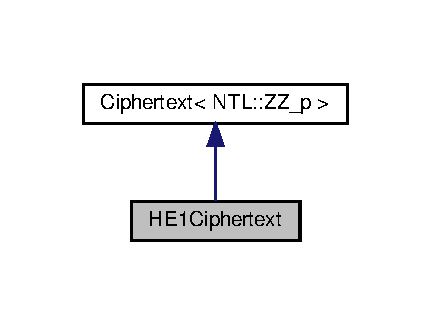
\includegraphics[width=207pt]{classHE1Ciphertext__inherit__graph}
\end{center}
\end{figure}


Collaboration diagram for H\+E1\+Ciphertext\+:
\nopagebreak
\begin{figure}[H]
\begin{center}
\leavevmode
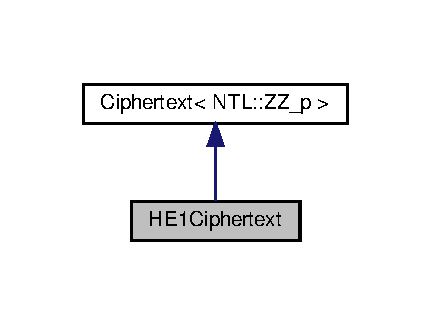
\includegraphics[width=207pt]{classHE1Ciphertext__coll__graph}
\end{center}
\end{figure}
\subsection*{Public Member Functions}
\begin{DoxyCompactItemize}
\item 
\hyperlink{classHE1Ciphertext_afd58548a4f93ef8576f35677fa42e35c}{H\+E1\+Ciphertext} ()
\item 
\hyperlink{classHE1Ciphertext_a4956d0c93fecd2db56a51e77f6f959ef}{H\+E1\+Ciphertext} (N\+T\+L\+::\+Z\+Z\+\_\+p \&\hyperlink{classCiphertext_adef9aae9d923eb100b4a1ad58ce495f1}{ciphertext})
\item 
\hyperlink{classHE1Ciphertext_a178b26d8b0a54d3e1e0e5bb04bb09bd6}{H\+E1\+Ciphertext} (N\+T\+L\+::\+ZZ \&\hyperlink{classCiphertext_adef9aae9d923eb100b4a1ad58ce495f1}{ciphertext})
\item 
\hyperlink{classHE1Ciphertext_a1f1b6b024af4615bc3a54025c42382dc}{H\+E1\+Ciphertext} (std\+::string \&str)
\item 
virtual \hyperlink{classHE1Ciphertext_ab5b083f4f4d980d127751df627b976e9}{$\sim$\+H\+E1\+Ciphertext} ()
\item 
\hyperlink{classHE1Ciphertext}{H\+E1\+Ciphertext} \& \hyperlink{classHE1Ciphertext_a3ce293f9fd8d25c2921c589bb8f8c171}{operator+=} (const \hyperlink{classHE1Ciphertext}{H\+E1\+Ciphertext} \&o)
\item 
\hyperlink{classHE1Ciphertext}{H\+E1\+Ciphertext} \& \hyperlink{classHE1Ciphertext_ab2eb089852b2d0155c4da6080886a75a}{operator$\ast$=} (const \hyperlink{classHE1Ciphertext}{H\+E1\+Ciphertext} \&o)
\end{DoxyCompactItemize}
\subsection*{Static Public Member Functions}
\begin{DoxyCompactItemize}
\item 
static void \hyperlink{classHE1Ciphertext_a3cf78bc8d18c72fbb8bd116447371bf2}{set\+Modulus} (N\+T\+L\+::\+ZZ \&\hyperlink{classHE1Ciphertext_a924bd87bcc91518945bc039f10a20a48}{modulus})
\item 
static void \hyperlink{classHE1Ciphertext_a7b9c00baa1bfa692cfa518f98a46da78}{set\+Modulus} (std\+::string \&parameters)
\end{DoxyCompactItemize}
\subsection*{Private Member Functions}
\begin{DoxyCompactItemize}
\item 
{\footnotesize template$<$class Archive $>$ }\\void \hyperlink{classHE1Ciphertext_a2868e8110f81031f5e6263e97a3232c0}{save} (Archive \&ar, const unsigned int version) const
\item 
{\footnotesize template$<$class Archive $>$ }\\void \hyperlink{classHE1Ciphertext_a8a9024694e1826459a53be0c7a82925e}{load} (Archive \&ar, const unsigned int version)
\item 
{\footnotesize template$<$class Archive $>$ }\\void \hyperlink{classHE1Ciphertext_ac2c27abc00dbef4ea47d7b4a3588dd1c}{serialize} (Archive \&ar, const unsigned int version)
\end{DoxyCompactItemize}
\subsection*{Static Private Attributes}
\begin{DoxyCompactItemize}
\item 
static N\+T\+L\+::\+ZZ \hyperlink{classHE1Ciphertext_a924bd87bcc91518945bc039f10a20a48}{modulus}
\end{DoxyCompactItemize}
\subsection*{Friends}
\begin{DoxyCompactItemize}
\item 
class \hyperlink{classHE1Ciphertext_ac98d07dd8f7b70e16ccb9a01abf56b9c}{boost\+::serialization\+::access}
\item 
std\+::ostream \& \hyperlink{classHE1Ciphertext_a684afdb22c43258ab0e2e5ab73abaed0}{operator$<$$<$} (std\+::ostream \&o, const \hyperlink{classHE1Ciphertext}{H\+E1\+Ciphertext} \&c)
\item 
std\+::istream \& \hyperlink{classHE1Ciphertext_a1e2c0400cdd3fca5fcd4946f9b053b8c}{operator$>$$>$} (std\+::istream \&i, const \hyperlink{classHE1Ciphertext}{H\+E1\+Ciphertext} \&c)
\item 
\hyperlink{classHE1Ciphertext}{H\+E1\+Ciphertext} \hyperlink{classHE1Ciphertext_a2e914308f6b7d88f63067fca516f4055}{operator+} (const \hyperlink{classHE1Ciphertext}{H\+E1\+Ciphertext} \&a, const \hyperlink{classHE1Ciphertext}{H\+E1\+Ciphertext} \&b)
\item 
\hyperlink{classHE1Ciphertext}{H\+E1\+Ciphertext} \hyperlink{classHE1Ciphertext_a8b5554bdd70338b6c916db1423702314}{operator$\ast$} (const \hyperlink{classHE1Ciphertext}{H\+E1\+Ciphertext} \&a, const \hyperlink{classHE1Ciphertext}{H\+E1\+Ciphertext} \&b)
\end{DoxyCompactItemize}
\subsection*{Additional Inherited Members}


\subsection{Constructor \& Destructor Documentation}
\mbox{\Hypertarget{classHE1Ciphertext_afd58548a4f93ef8576f35677fa42e35c}\label{classHE1Ciphertext_afd58548a4f93ef8576f35677fa42e35c}} 
\index{H\+E1\+Ciphertext@{H\+E1\+Ciphertext}!H\+E1\+Ciphertext@{H\+E1\+Ciphertext}}
\index{H\+E1\+Ciphertext@{H\+E1\+Ciphertext}!H\+E1\+Ciphertext@{H\+E1\+Ciphertext}}
\subsubsection{\texorpdfstring{H\+E1\+Ciphertext()}{HE1Ciphertext()}\hspace{0.1cm}{\footnotesize\ttfamily [1/4]}}
{\footnotesize\ttfamily H\+E1\+Ciphertext\+::\+H\+E1\+Ciphertext (\begin{DoxyParamCaption}{ }\end{DoxyParamCaption})}

Default constructor \mbox{\Hypertarget{classHE1Ciphertext_a4956d0c93fecd2db56a51e77f6f959ef}\label{classHE1Ciphertext_a4956d0c93fecd2db56a51e77f6f959ef}} 
\index{H\+E1\+Ciphertext@{H\+E1\+Ciphertext}!H\+E1\+Ciphertext@{H\+E1\+Ciphertext}}
\index{H\+E1\+Ciphertext@{H\+E1\+Ciphertext}!H\+E1\+Ciphertext@{H\+E1\+Ciphertext}}
\subsubsection{\texorpdfstring{H\+E1\+Ciphertext()}{HE1Ciphertext()}\hspace{0.1cm}{\footnotesize\ttfamily [2/4]}}
{\footnotesize\ttfamily H\+E1\+Ciphertext\+::\+H\+E1\+Ciphertext (\begin{DoxyParamCaption}\item[{N\+T\+L\+::\+Z\+Z\+\_\+p \&}]{ciphertext }\end{DoxyParamCaption})}

Initialise {\ttfamily ciphertext} with the supplied value 
\begin{DoxyParams}{Parameters}
{\em ciphertext} & An N\+TL multiprecision modular integer \\
\hline
\end{DoxyParams}
\mbox{\Hypertarget{classHE1Ciphertext_a178b26d8b0a54d3e1e0e5bb04bb09bd6}\label{classHE1Ciphertext_a178b26d8b0a54d3e1e0e5bb04bb09bd6}} 
\index{H\+E1\+Ciphertext@{H\+E1\+Ciphertext}!H\+E1\+Ciphertext@{H\+E1\+Ciphertext}}
\index{H\+E1\+Ciphertext@{H\+E1\+Ciphertext}!H\+E1\+Ciphertext@{H\+E1\+Ciphertext}}
\subsubsection{\texorpdfstring{H\+E1\+Ciphertext()}{HE1Ciphertext()}\hspace{0.1cm}{\footnotesize\ttfamily [3/4]}}
{\footnotesize\ttfamily H\+E1\+Ciphertext\+::\+H\+E1\+Ciphertext (\begin{DoxyParamCaption}\item[{N\+T\+L\+::\+ZZ \&}]{ciphertext }\end{DoxyParamCaption})}

Initialise {\ttfamily ciphertext} with the supplied value 
\begin{DoxyParams}{Parameters}
{\em ciphertext} & An N\+TL multiprecision integer \\
\hline
\end{DoxyParams}
\mbox{\Hypertarget{classHE1Ciphertext_a1f1b6b024af4615bc3a54025c42382dc}\label{classHE1Ciphertext_a1f1b6b024af4615bc3a54025c42382dc}} 
\index{H\+E1\+Ciphertext@{H\+E1\+Ciphertext}!H\+E1\+Ciphertext@{H\+E1\+Ciphertext}}
\index{H\+E1\+Ciphertext@{H\+E1\+Ciphertext}!H\+E1\+Ciphertext@{H\+E1\+Ciphertext}}
\subsubsection{\texorpdfstring{H\+E1\+Ciphertext()}{HE1Ciphertext()}\hspace{0.1cm}{\footnotesize\ttfamily [4/4]}}
{\footnotesize\ttfamily H\+E1\+Ciphertext\+::\+H\+E1\+Ciphertext (\begin{DoxyParamCaption}\item[{std\+::string \&}]{str }\end{DoxyParamCaption})}

Initialise {\ttfamily ciphertext} with the supplied decimal string 
\begin{DoxyParams}{Parameters}
{\em str} & A decimal string \\
\hline
\end{DoxyParams}
\mbox{\Hypertarget{classHE1Ciphertext_ab5b083f4f4d980d127751df627b976e9}\label{classHE1Ciphertext_ab5b083f4f4d980d127751df627b976e9}} 
\index{H\+E1\+Ciphertext@{H\+E1\+Ciphertext}!````~H\+E1\+Ciphertext@{$\sim$\+H\+E1\+Ciphertext}}
\index{````~H\+E1\+Ciphertext@{$\sim$\+H\+E1\+Ciphertext}!H\+E1\+Ciphertext@{H\+E1\+Ciphertext}}
\subsubsection{\texorpdfstring{$\sim$\+H\+E1\+Ciphertext()}{~HE1Ciphertext()}}
{\footnotesize\ttfamily H\+E1\+Ciphertext\+::$\sim$\+H\+E1\+Ciphertext (\begin{DoxyParamCaption}{ }\end{DoxyParamCaption})\hspace{0.3cm}{\ttfamily [virtual]}}

Default destuctor 

\subsection{Member Function Documentation}
\mbox{\Hypertarget{classHE1Ciphertext_a8a9024694e1826459a53be0c7a82925e}\label{classHE1Ciphertext_a8a9024694e1826459a53be0c7a82925e}} 
\index{H\+E1\+Ciphertext@{H\+E1\+Ciphertext}!load@{load}}
\index{load@{load}!H\+E1\+Ciphertext@{H\+E1\+Ciphertext}}
\subsubsection{\texorpdfstring{load()}{load()}}
{\footnotesize\ttfamily template$<$class Archive $>$ \\
void H\+E1\+Ciphertext\+::load (\begin{DoxyParamCaption}\item[{Archive \&}]{ar,  }\item[{const unsigned int}]{version }\end{DoxyParamCaption})\hspace{0.3cm}{\ttfamily [inline]}, {\ttfamily [private]}}

Deserialise object from archive 
\begin{DoxyParams}{Parameters}
{\em ar} & An archive \\
\hline
{\em version} & Class version \\
\hline
\end{DoxyParams}
\mbox{\Hypertarget{classHE1Ciphertext_ab2eb089852b2d0155c4da6080886a75a}\label{classHE1Ciphertext_ab2eb089852b2d0155c4da6080886a75a}} 
\index{H\+E1\+Ciphertext@{H\+E1\+Ciphertext}!operator$\ast$=@{operator$\ast$=}}
\index{operator$\ast$=@{operator$\ast$=}!H\+E1\+Ciphertext@{H\+E1\+Ciphertext}}
\subsubsection{\texorpdfstring{operator$\ast$=()}{operator*=()}}
{\footnotesize\ttfamily \hyperlink{classHE1Ciphertext}{H\+E1\+Ciphertext} \& H\+E1\+Ciphertext\+::operator$\ast$= (\begin{DoxyParamCaption}\item[{const \hyperlink{classHE1Ciphertext}{H\+E1\+Ciphertext} \&}]{o }\end{DoxyParamCaption})}

Performs modular multiplication of {\ttfamily this.\+ciphertext} and {\ttfamily o.\+ciphertext}. Assigns result to {\ttfamily this.\+ciphertext} 
\begin{DoxyParams}{Parameters}
{\em o} & {\ttfamily \hyperlink{classHE1Ciphertext}{H\+E1\+Ciphertext}} object \\
\hline
\end{DoxyParams}
\begin{DoxyReturn}{Returns}
{\ttfamily this} 
\end{DoxyReturn}
\mbox{\Hypertarget{classHE1Ciphertext_a3ce293f9fd8d25c2921c589bb8f8c171}\label{classHE1Ciphertext_a3ce293f9fd8d25c2921c589bb8f8c171}} 
\index{H\+E1\+Ciphertext@{H\+E1\+Ciphertext}!operator+=@{operator+=}}
\index{operator+=@{operator+=}!H\+E1\+Ciphertext@{H\+E1\+Ciphertext}}
\subsubsection{\texorpdfstring{operator+=()}{operator+=()}}
{\footnotesize\ttfamily \hyperlink{classHE1Ciphertext}{H\+E1\+Ciphertext} \& H\+E1\+Ciphertext\+::operator+= (\begin{DoxyParamCaption}\item[{const \hyperlink{classHE1Ciphertext}{H\+E1\+Ciphertext} \&}]{o }\end{DoxyParamCaption})}

Performs modular addition of {\ttfamily this.\+ciphertext} and {\ttfamily o.\+ciphertext}. Assigns result to {\ttfamily this.\+ciphertext} 
\begin{DoxyParams}{Parameters}
{\em o} & {\ttfamily \hyperlink{classHE1Ciphertext}{H\+E1\+Ciphertext}} object \\
\hline
\end{DoxyParams}
\begin{DoxyReturn}{Returns}
{\ttfamily this} 
\end{DoxyReturn}
\mbox{\Hypertarget{classHE1Ciphertext_a2868e8110f81031f5e6263e97a3232c0}\label{classHE1Ciphertext_a2868e8110f81031f5e6263e97a3232c0}} 
\index{H\+E1\+Ciphertext@{H\+E1\+Ciphertext}!save@{save}}
\index{save@{save}!H\+E1\+Ciphertext@{H\+E1\+Ciphertext}}
\subsubsection{\texorpdfstring{save()}{save()}}
{\footnotesize\ttfamily template$<$class Archive $>$ \\
void H\+E1\+Ciphertext\+::save (\begin{DoxyParamCaption}\item[{Archive \&}]{ar,  }\item[{const unsigned int}]{version }\end{DoxyParamCaption}) const\hspace{0.3cm}{\ttfamily [inline]}, {\ttfamily [private]}}

Serialise object to archive. 
\begin{DoxyParams}{Parameters}
{\em ar} & An archive \\
\hline
{\em version} & Class version \\
\hline
\end{DoxyParams}
\mbox{\Hypertarget{classHE1Ciphertext_ac2c27abc00dbef4ea47d7b4a3588dd1c}\label{classHE1Ciphertext_ac2c27abc00dbef4ea47d7b4a3588dd1c}} 
\index{H\+E1\+Ciphertext@{H\+E1\+Ciphertext}!serialize@{serialize}}
\index{serialize@{serialize}!H\+E1\+Ciphertext@{H\+E1\+Ciphertext}}
\subsubsection{\texorpdfstring{serialize()}{serialize()}}
{\footnotesize\ttfamily template$<$class Archive $>$ \\
void H\+E1\+Ciphertext\+::serialize (\begin{DoxyParamCaption}\item[{Archive \&}]{ar,  }\item[{const unsigned int}]{version }\end{DoxyParamCaption})\hspace{0.3cm}{\ttfamily [inline]}, {\ttfamily [private]}}

Bidirectional serialisation of this object \begin{DoxySeeAlso}{See also}
\hyperlink{classHE1Ciphertext_a2868e8110f81031f5e6263e97a3232c0}{save} 

\hyperlink{classHE1Ciphertext_a8a9024694e1826459a53be0c7a82925e}{load} 
\end{DoxySeeAlso}

\begin{DoxyParams}{Parameters}
{\em ar} & An Archive \\
\hline
{\em version} & Class version \\
\hline
\end{DoxyParams}
\mbox{\Hypertarget{classHE1Ciphertext_a3cf78bc8d18c72fbb8bd116447371bf2}\label{classHE1Ciphertext_a3cf78bc8d18c72fbb8bd116447371bf2}} 
\index{H\+E1\+Ciphertext@{H\+E1\+Ciphertext}!set\+Modulus@{set\+Modulus}}
\index{set\+Modulus@{set\+Modulus}!H\+E1\+Ciphertext@{H\+E1\+Ciphertext}}
\subsubsection{\texorpdfstring{set\+Modulus()}{setModulus()}\hspace{0.1cm}{\footnotesize\ttfamily [1/2]}}
{\footnotesize\ttfamily void H\+E1\+Ciphertext\+::set\+Modulus (\begin{DoxyParamCaption}\item[{N\+T\+L\+::\+ZZ \&}]{mod }\end{DoxyParamCaption})\hspace{0.3cm}{\ttfamily [static]}}

Sets the public modulus 
\begin{DoxyParams}{Parameters}
{\em mod} & An N\+TL multiprecision integer \\
\hline
\end{DoxyParams}
\mbox{\Hypertarget{classHE1Ciphertext_a7b9c00baa1bfa692cfa518f98a46da78}\label{classHE1Ciphertext_a7b9c00baa1bfa692cfa518f98a46da78}} 
\index{H\+E1\+Ciphertext@{H\+E1\+Ciphertext}!set\+Modulus@{set\+Modulus}}
\index{set\+Modulus@{set\+Modulus}!H\+E1\+Ciphertext@{H\+E1\+Ciphertext}}
\subsubsection{\texorpdfstring{set\+Modulus()}{setModulus()}\hspace{0.1cm}{\footnotesize\ttfamily [2/2]}}
{\footnotesize\ttfamily void H\+E1\+Ciphertext\+::set\+Modulus (\begin{DoxyParamCaption}\item[{std\+::string \&}]{parameters }\end{DoxyParamCaption})\hspace{0.3cm}{\ttfamily [static]}}

Sets the public modulus from a J\+S\+ON String 
\begin{DoxyParams}{Parameters}
{\em parameters} & A J\+S\+ON string \\
\hline
\end{DoxyParams}


\subsection{Friends And Related Function Documentation}
\mbox{\Hypertarget{classHE1Ciphertext_ac98d07dd8f7b70e16ccb9a01abf56b9c}\label{classHE1Ciphertext_ac98d07dd8f7b70e16ccb9a01abf56b9c}} 
\index{H\+E1\+Ciphertext@{H\+E1\+Ciphertext}!boost\+::serialization\+::access@{boost\+::serialization\+::access}}
\index{boost\+::serialization\+::access@{boost\+::serialization\+::access}!H\+E1\+Ciphertext@{H\+E1\+Ciphertext}}
\subsubsection{\texorpdfstring{boost\+::serialization\+::access}{boost::serialization::access}}
{\footnotesize\ttfamily friend class boost\+::serialization\+::access\hspace{0.3cm}{\ttfamily [friend]}}

\mbox{\Hypertarget{classHE1Ciphertext_a8b5554bdd70338b6c916db1423702314}\label{classHE1Ciphertext_a8b5554bdd70338b6c916db1423702314}} 
\index{H\+E1\+Ciphertext@{H\+E1\+Ciphertext}!operator$\ast$@{operator$\ast$}}
\index{operator$\ast$@{operator$\ast$}!H\+E1\+Ciphertext@{H\+E1\+Ciphertext}}
\subsubsection{\texorpdfstring{operator$\ast$}{operator*}}
{\footnotesize\ttfamily \hyperlink{classHE1Ciphertext}{H\+E1\+Ciphertext} operator$\ast$ (\begin{DoxyParamCaption}\item[{const \hyperlink{classHE1Ciphertext}{H\+E1\+Ciphertext} \&}]{a,  }\item[{const \hyperlink{classHE1Ciphertext}{H\+E1\+Ciphertext} \&}]{b }\end{DoxyParamCaption})\hspace{0.3cm}{\ttfamily [friend]}}

Performs modular multiplication of {\ttfamily a.\+ciphertext} and {\ttfamily b.\+ciphertext} 
\begin{DoxyParams}{Parameters}
{\em a} & {\ttfamily \hyperlink{classHE1Ciphertext}{H\+E1\+Ciphertext}} object \\
\hline
{\em b} & {\ttfamily \hyperlink{classHE1Ciphertext}{H\+E1\+Ciphertext}} object \\
\hline
\end{DoxyParams}
\begin{DoxyReturn}{Returns}
{\ttfamily \hyperlink{classHE1Ciphertext}{H\+E1\+Ciphertext}} object containing the product 
\end{DoxyReturn}
\mbox{\Hypertarget{classHE1Ciphertext_a2e914308f6b7d88f63067fca516f4055}\label{classHE1Ciphertext_a2e914308f6b7d88f63067fca516f4055}} 
\index{H\+E1\+Ciphertext@{H\+E1\+Ciphertext}!operator+@{operator+}}
\index{operator+@{operator+}!H\+E1\+Ciphertext@{H\+E1\+Ciphertext}}
\subsubsection{\texorpdfstring{operator+}{operator+}}
{\footnotesize\ttfamily \hyperlink{classHE1Ciphertext}{H\+E1\+Ciphertext} operator+ (\begin{DoxyParamCaption}\item[{const \hyperlink{classHE1Ciphertext}{H\+E1\+Ciphertext} \&}]{a,  }\item[{const \hyperlink{classHE1Ciphertext}{H\+E1\+Ciphertext} \&}]{b }\end{DoxyParamCaption})\hspace{0.3cm}{\ttfamily [friend]}}

Performs modular addition of {\ttfamily a.\+ciphertext} and {\ttfamily b.\+ciphertext} 
\begin{DoxyParams}{Parameters}
{\em a} & {\ttfamily \hyperlink{classHE1Ciphertext}{H\+E1\+Ciphertext}} object \\
\hline
{\em b} & {\ttfamily \hyperlink{classHE1Ciphertext}{H\+E1\+Ciphertext}} object \\
\hline
\end{DoxyParams}
\begin{DoxyReturn}{Returns}
{\ttfamily \hyperlink{classHE1Ciphertext}{H\+E1\+Ciphertext}} object containing the sum 
\end{DoxyReturn}
\mbox{\Hypertarget{classHE1Ciphertext_a684afdb22c43258ab0e2e5ab73abaed0}\label{classHE1Ciphertext_a684afdb22c43258ab0e2e5ab73abaed0}} 
\index{H\+E1\+Ciphertext@{H\+E1\+Ciphertext}!operator$<$$<$@{operator$<$$<$}}
\index{operator$<$$<$@{operator$<$$<$}!H\+E1\+Ciphertext@{H\+E1\+Ciphertext}}
\subsubsection{\texorpdfstring{operator$<$$<$}{operator<<}}
{\footnotesize\ttfamily std\+::ostream\& operator$<$$<$ (\begin{DoxyParamCaption}\item[{std\+::ostream \&}]{o,  }\item[{const \hyperlink{classHE1Ciphertext}{H\+E1\+Ciphertext} \&}]{c }\end{DoxyParamCaption})\hspace{0.3cm}{\ttfamily [friend]}}

Write {\ttfamily ciphertext} to output stream as decimal string 
\begin{DoxyParams}{Parameters}
{\em o} & Output stream \\
\hline
{\em c} & {\ttfamily \hyperlink{classHE1Ciphertext}{H\+E1\+Ciphertext}} object \\
\hline
\end{DoxyParams}
\begin{DoxyReturn}{Returns}
A reference to the output stream 
\end{DoxyReturn}
\mbox{\Hypertarget{classHE1Ciphertext_a1e2c0400cdd3fca5fcd4946f9b053b8c}\label{classHE1Ciphertext_a1e2c0400cdd3fca5fcd4946f9b053b8c}} 
\index{H\+E1\+Ciphertext@{H\+E1\+Ciphertext}!operator$>$$>$@{operator$>$$>$}}
\index{operator$>$$>$@{operator$>$$>$}!H\+E1\+Ciphertext@{H\+E1\+Ciphertext}}
\subsubsection{\texorpdfstring{operator$>$$>$}{operator>>}}
{\footnotesize\ttfamily std\+::istream\& operator$>$$>$ (\begin{DoxyParamCaption}\item[{std\+::istream \&}]{i,  }\item[{const \hyperlink{classHE1Ciphertext}{H\+E1\+Ciphertext} \&}]{c }\end{DoxyParamCaption})\hspace{0.3cm}{\ttfamily [friend]}}



\subsection{Member Data Documentation}
\mbox{\Hypertarget{classHE1Ciphertext_a924bd87bcc91518945bc039f10a20a48}\label{classHE1Ciphertext_a924bd87bcc91518945bc039f10a20a48}} 
\index{H\+E1\+Ciphertext@{H\+E1\+Ciphertext}!modulus@{modulus}}
\index{modulus@{modulus}!H\+E1\+Ciphertext@{H\+E1\+Ciphertext}}
\subsubsection{\texorpdfstring{modulus}{modulus}}
{\footnotesize\ttfamily N\+T\+L\+::\+ZZ H\+E1\+Ciphertext\+::modulus\hspace{0.3cm}{\ttfamily [static]}, {\ttfamily [private]}}

A public cipher parameter\+: the modulus for arithmetic 

The documentation for this class was generated from the following files\+:\begin{DoxyCompactItemize}
\item 
include/\hyperlink{HE1Ciphertext_8h}{H\+E1\+Ciphertext.\+h}\item 
src/\hyperlink{HE1Ciphertext_8cpp}{H\+E1\+Ciphertext.\+cpp}\end{DoxyCompactItemize}

\hypertarget{classHE2Ciphertext}{}\section{H\+E2\+Ciphertext Class Reference}
\label{classHE2Ciphertext}\index{H\+E2\+Ciphertext@{H\+E2\+Ciphertext}}


{\ttfamily \#include $<$H\+E2\+Ciphertext.\+h$>$}



Inheritance diagram for H\+E2\+Ciphertext\+:
\nopagebreak
\begin{figure}[H]
\begin{center}
\leavevmode
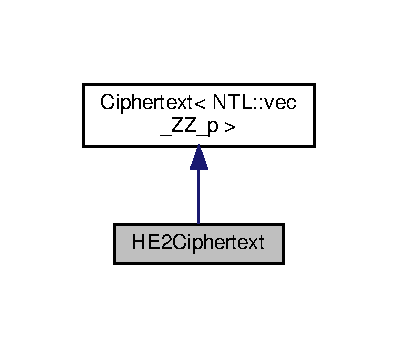
\includegraphics[width=191pt]{classHE2Ciphertext__inherit__graph}
\end{center}
\end{figure}


Collaboration diagram for H\+E2\+Ciphertext\+:
\nopagebreak
\begin{figure}[H]
\begin{center}
\leavevmode
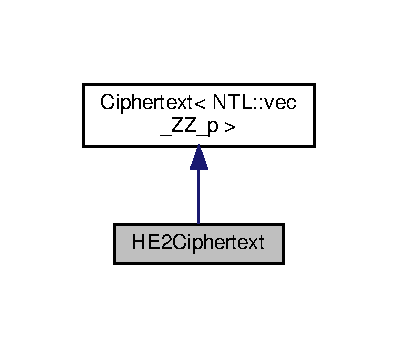
\includegraphics[width=191pt]{classHE2Ciphertext__coll__graph}
\end{center}
\end{figure}
\subsection*{Public Member Functions}
\begin{DoxyCompactItemize}
\item 
\hyperlink{classHE2Ciphertext_ad5bfed280b98c618f55fb7bf28a7b1cd}{H\+E2\+Ciphertext} ()
\item 
\hyperlink{classHE2Ciphertext_a8d74aeeaa1af989e7e033f5f35c54550}{H\+E2\+Ciphertext} (N\+T\+L\+::vec\+\_\+\+Z\+Z\+\_\+p \&\hyperlink{classCiphertext_adef9aae9d923eb100b4a1ad58ce495f1}{ciphertext})
\item 
\hyperlink{classHE2Ciphertext_a3c8e2e1657aab1597223ed3b04cdff0e}{H\+E2\+Ciphertext} (N\+T\+L\+::vec\+\_\+\+ZZ \&\hyperlink{classCiphertext_adef9aae9d923eb100b4a1ad58ce495f1}{ciphertext})
\item 
\hyperlink{classHE2Ciphertext_a0b43eb4010e5dcb24c185b16f96fdf18}{H\+E2\+Ciphertext} (std\+::string \&str)
\item 
virtual \hyperlink{classHE2Ciphertext_a5acc06ab4a495f477c43814bea877dcd}{$\sim$\+H\+E2\+Ciphertext} ()
\item 
\hyperlink{classHE2Ciphertext}{H\+E2\+Ciphertext} \& \hyperlink{classHE2Ciphertext_a5c54fb70a082d42607ed6923b9d9118b}{operator+=} (const \hyperlink{classHE2Ciphertext}{H\+E2\+Ciphertext} \&o)
\item 
\hyperlink{classHE2Ciphertext}{H\+E2\+Ciphertext} \& \hyperlink{classHE2Ciphertext_aa0502b251b22d25db90ef16bc2f05122}{operator$\ast$=} (const \hyperlink{classHE2Ciphertext}{H\+E2\+Ciphertext} \&o)
\end{DoxyCompactItemize}
\subsection*{Static Public Member Functions}
\begin{DoxyCompactItemize}
\item 
static void \hyperlink{classHE2Ciphertext_afb27eefed819559aaebdaf0eb10d7311}{set\+Modulus} (N\+T\+L\+::\+ZZ \&\hyperlink{classHE2Ciphertext_a590c7d8432a2a73ebe0607f402c6a46a}{modulus})
\item 
static void \hyperlink{classHE2Ciphertext_a8369345555e2b6df742e238353bd8707}{set\+Matrix} (N\+T\+L\+::mat\+\_\+\+Z\+Z\+\_\+p $\ast$\hyperlink{classHE2Ciphertext_aad6e0d90aa41cb80b75feebc1b07e1c0}{R})
\item 
static void \hyperlink{classHE2Ciphertext_ae3b1a39f8c20cc4d97bcc1ea70cf641e}{set\+Parameters} (std\+::string \&parameters)
\end{DoxyCompactItemize}
\subsection*{Private Member Functions}
\begin{DoxyCompactItemize}
\item 
{\footnotesize template$<$class Archive $>$ }\\void \hyperlink{classHE2Ciphertext_a0fcff8ec1b87d67f22da109ba9cc4931}{save} (Archive \&ar, const unsigned int version) const
\item 
{\footnotesize template$<$class Archive $>$ }\\void \hyperlink{classHE2Ciphertext_a2cfa63d6dacdb977ecf6a0043b207b92}{load} (Archive \&ar, const unsigned int version)
\item 
{\footnotesize template$<$class Archive $>$ }\\void \hyperlink{classHE2Ciphertext_a143f80d41791ba3eff4f76b43734daec}{serialize} (Archive \&ar, const unsigned int version)
\end{DoxyCompactItemize}
\subsection*{Static Private Member Functions}
\begin{DoxyCompactItemize}
\item 
static N\+T\+L\+::vec\+\_\+\+Z\+Z\+\_\+p \hyperlink{classHE2Ciphertext_af8e0dca1959cf2cbd7606d48476c435a}{augment} (const N\+T\+L\+::vec\+\_\+\+Z\+Z\+\_\+p \&v)
\item 
static N\+T\+L\+::vec\+\_\+\+Z\+Z\+\_\+p \hyperlink{classHE2Ciphertext_a30047cae60f901b106371d70027bf286}{product} (const N\+T\+L\+::vec\+\_\+\+Z\+Z\+\_\+p \&a, const N\+T\+L\+::vec\+\_\+\+Z\+Z\+\_\+p \&b)
\end{DoxyCompactItemize}
\subsection*{Static Private Attributes}
\begin{DoxyCompactItemize}
\item 
static N\+T\+L\+::\+ZZ \hyperlink{classHE2Ciphertext_a590c7d8432a2a73ebe0607f402c6a46a}{modulus}
\item 
static N\+T\+L\+::mat\+\_\+\+Z\+Z\+\_\+p $\ast$ \hyperlink{classHE2Ciphertext_aad6e0d90aa41cb80b75feebc1b07e1c0}{R}
\end{DoxyCompactItemize}
\subsection*{Friends}
\begin{DoxyCompactItemize}
\item 
class \hyperlink{classHE2Ciphertext_ac98d07dd8f7b70e16ccb9a01abf56b9c}{boost\+::serialization\+::access}
\item 
std\+::ostream \& \hyperlink{classHE2Ciphertext_a5d9b4ffb87a447db8b95de9c64401e0f}{operator$<$$<$} (std\+::ostream \&o, const \hyperlink{classHE2Ciphertext}{H\+E2\+Ciphertext} \&c)
\item 
std\+::istream \& \hyperlink{classHE2Ciphertext_a8cd6e8f36f12e9b0548d6f66fae71816}{operator$>$$>$} (std\+::istream \&i, \hyperlink{classHE2Ciphertext}{H\+E2\+Ciphertext} \&c)
\item 
\hyperlink{classHE2Ciphertext}{H\+E2\+Ciphertext} \hyperlink{classHE2Ciphertext_af90fd206e69fa74b30d40f41f707bdb8}{operator+} (const \hyperlink{classHE2Ciphertext}{H\+E2\+Ciphertext} \&a, const \hyperlink{classHE2Ciphertext}{H\+E2\+Ciphertext} \&b)
\item 
\hyperlink{classHE2Ciphertext}{H\+E2\+Ciphertext} \hyperlink{classHE2Ciphertext_adfb636b8ce661b0edbd9297cdcf61c88}{operator$\ast$} (const \hyperlink{classHE2Ciphertext}{H\+E2\+Ciphertext} \&a, const \hyperlink{classHE2Ciphertext}{H\+E2\+Ciphertext} \&b)
\end{DoxyCompactItemize}
\subsection*{Additional Inherited Members}


\subsection{Constructor \& Destructor Documentation}
\mbox{\Hypertarget{classHE2Ciphertext_ad5bfed280b98c618f55fb7bf28a7b1cd}\label{classHE2Ciphertext_ad5bfed280b98c618f55fb7bf28a7b1cd}} 
\index{H\+E2\+Ciphertext@{H\+E2\+Ciphertext}!H\+E2\+Ciphertext@{H\+E2\+Ciphertext}}
\index{H\+E2\+Ciphertext@{H\+E2\+Ciphertext}!H\+E2\+Ciphertext@{H\+E2\+Ciphertext}}
\subsubsection{\texorpdfstring{H\+E2\+Ciphertext()}{HE2Ciphertext()}\hspace{0.1cm}{\footnotesize\ttfamily [1/4]}}
{\footnotesize\ttfamily H\+E2\+Ciphertext\+::\+H\+E2\+Ciphertext (\begin{DoxyParamCaption}{ }\end{DoxyParamCaption})}

Default constructor \mbox{\Hypertarget{classHE2Ciphertext_a8d74aeeaa1af989e7e033f5f35c54550}\label{classHE2Ciphertext_a8d74aeeaa1af989e7e033f5f35c54550}} 
\index{H\+E2\+Ciphertext@{H\+E2\+Ciphertext}!H\+E2\+Ciphertext@{H\+E2\+Ciphertext}}
\index{H\+E2\+Ciphertext@{H\+E2\+Ciphertext}!H\+E2\+Ciphertext@{H\+E2\+Ciphertext}}
\subsubsection{\texorpdfstring{H\+E2\+Ciphertext()}{HE2Ciphertext()}\hspace{0.1cm}{\footnotesize\ttfamily [2/4]}}
{\footnotesize\ttfamily H\+E2\+Ciphertext\+::\+H\+E2\+Ciphertext (\begin{DoxyParamCaption}\item[{N\+T\+L\+::vec\+\_\+\+Z\+Z\+\_\+p \&}]{ciphertext }\end{DoxyParamCaption})}

Initialize {\ttfamily ciphertext} with the value supplied 
\begin{DoxyParams}{Parameters}
{\em ciphertext} & A 2-\/vector of multiprecision integers modulo {\ttfamily modulus} \\
\hline
\end{DoxyParams}
\mbox{\Hypertarget{classHE2Ciphertext_a3c8e2e1657aab1597223ed3b04cdff0e}\label{classHE2Ciphertext_a3c8e2e1657aab1597223ed3b04cdff0e}} 
\index{H\+E2\+Ciphertext@{H\+E2\+Ciphertext}!H\+E2\+Ciphertext@{H\+E2\+Ciphertext}}
\index{H\+E2\+Ciphertext@{H\+E2\+Ciphertext}!H\+E2\+Ciphertext@{H\+E2\+Ciphertext}}
\subsubsection{\texorpdfstring{H\+E2\+Ciphertext()}{HE2Ciphertext()}\hspace{0.1cm}{\footnotesize\ttfamily [3/4]}}
{\footnotesize\ttfamily H\+E2\+Ciphertext\+::\+H\+E2\+Ciphertext (\begin{DoxyParamCaption}\item[{N\+T\+L\+::vec\+\_\+\+ZZ \&}]{ciphertext }\end{DoxyParamCaption})}

Initialize {\ttfamily ciphertext} with the value supplied 
\begin{DoxyParams}{Parameters}
{\em ciphertext} & A 2-\/vector of multiprecision integers \\
\hline
\end{DoxyParams}
\mbox{\Hypertarget{classHE2Ciphertext_a0b43eb4010e5dcb24c185b16f96fdf18}\label{classHE2Ciphertext_a0b43eb4010e5dcb24c185b16f96fdf18}} 
\index{H\+E2\+Ciphertext@{H\+E2\+Ciphertext}!H\+E2\+Ciphertext@{H\+E2\+Ciphertext}}
\index{H\+E2\+Ciphertext@{H\+E2\+Ciphertext}!H\+E2\+Ciphertext@{H\+E2\+Ciphertext}}
\subsubsection{\texorpdfstring{H\+E2\+Ciphertext()}{HE2Ciphertext()}\hspace{0.1cm}{\footnotesize\ttfamily [4/4]}}
{\footnotesize\ttfamily H\+E2\+Ciphertext\+::\+H\+E2\+Ciphertext (\begin{DoxyParamCaption}\item[{std\+::string \&}]{str }\end{DoxyParamCaption})}

Initialize {\ttfamily ciphertext} with the string representation of a 2-\/vector 
\begin{DoxyParams}{Parameters}
{\em str} & String representation of a 2-\/vector \\
\hline
\end{DoxyParams}
\mbox{\Hypertarget{classHE2Ciphertext_a5acc06ab4a495f477c43814bea877dcd}\label{classHE2Ciphertext_a5acc06ab4a495f477c43814bea877dcd}} 
\index{H\+E2\+Ciphertext@{H\+E2\+Ciphertext}!````~H\+E2\+Ciphertext@{$\sim$\+H\+E2\+Ciphertext}}
\index{````~H\+E2\+Ciphertext@{$\sim$\+H\+E2\+Ciphertext}!H\+E2\+Ciphertext@{H\+E2\+Ciphertext}}
\subsubsection{\texorpdfstring{$\sim$\+H\+E2\+Ciphertext()}{~HE2Ciphertext()}}
{\footnotesize\ttfamily H\+E2\+Ciphertext\+::$\sim$\+H\+E2\+Ciphertext (\begin{DoxyParamCaption}{ }\end{DoxyParamCaption})\hspace{0.3cm}{\ttfamily [virtual]}}

Default destructor 

\subsection{Member Function Documentation}
\mbox{\Hypertarget{classHE2Ciphertext_af8e0dca1959cf2cbd7606d48476c435a}\label{classHE2Ciphertext_af8e0dca1959cf2cbd7606d48476c435a}} 
\index{H\+E2\+Ciphertext@{H\+E2\+Ciphertext}!augment@{augment}}
\index{augment@{augment}!H\+E2\+Ciphertext@{H\+E2\+Ciphertext}}
\subsubsection{\texorpdfstring{augment()}{augment()}}
{\footnotesize\ttfamily N\+T\+L\+::vec\+\_\+\+Z\+Z\+\_\+p H\+E2\+Ciphertext\+::augment (\begin{DoxyParamCaption}\item[{const N\+T\+L\+::vec\+\_\+\+Z\+Z\+\_\+p \&}]{v }\end{DoxyParamCaption})\hspace{0.3cm}{\ttfamily [static]}, {\ttfamily [private]}}

Constructs the augmented 3-\/vector for 2-\/vector {\ttfamily v}. 
\begin{DoxyParams}{Parameters}
{\em v} & An N\+TL vector of modular integers \\
\hline
\end{DoxyParams}
\begin{DoxyReturn}{Returns}
An N\+TL vector of modular integers 
\end{DoxyReturn}
\mbox{\Hypertarget{classHE2Ciphertext_a2cfa63d6dacdb977ecf6a0043b207b92}\label{classHE2Ciphertext_a2cfa63d6dacdb977ecf6a0043b207b92}} 
\index{H\+E2\+Ciphertext@{H\+E2\+Ciphertext}!load@{load}}
\index{load@{load}!H\+E2\+Ciphertext@{H\+E2\+Ciphertext}}
\subsubsection{\texorpdfstring{load()}{load()}}
{\footnotesize\ttfamily template$<$class Archive $>$ \\
void H\+E2\+Ciphertext\+::load (\begin{DoxyParamCaption}\item[{Archive \&}]{ar,  }\item[{const unsigned int}]{version }\end{DoxyParamCaption})\hspace{0.3cm}{\ttfamily [inline]}, {\ttfamily [private]}}

\mbox{\Hypertarget{classHE2Ciphertext_aa0502b251b22d25db90ef16bc2f05122}\label{classHE2Ciphertext_aa0502b251b22d25db90ef16bc2f05122}} 
\index{H\+E2\+Ciphertext@{H\+E2\+Ciphertext}!operator$\ast$=@{operator$\ast$=}}
\index{operator$\ast$=@{operator$\ast$=}!H\+E2\+Ciphertext@{H\+E2\+Ciphertext}}
\subsubsection{\texorpdfstring{operator$\ast$=()}{operator*=()}}
{\footnotesize\ttfamily \hyperlink{classHE2Ciphertext}{H\+E2\+Ciphertext} \& H\+E2\+Ciphertext\+::operator$\ast$= (\begin{DoxyParamCaption}\item[{const \hyperlink{classHE2Ciphertext}{H\+E2\+Ciphertext} \&}]{o }\end{DoxyParamCaption})}

Multiply the ciphertexts and assign to this objects {\ttfamily ciphertext} member. In the context of the H\+E2 ciphers, multiplication is the Hadamard product (\begin{DoxySeeAlso}{See also}
\hyperlink{classHE2Ciphertext_a30047cae60f901b106371d70027bf286}{product}) of augmented vectors (

\hyperlink{classHE2Ciphertext_af8e0dca1959cf2cbd7606d48476c435a}{augment}), followed by multiplication by the matrix {\ttfamily \hyperlink{classHE2Ciphertext_aad6e0d90aa41cb80b75feebc1b07e1c0}{R}}. 
\end{DoxySeeAlso}

\begin{DoxyParams}{Parameters}
{\em o} & Another {\ttfamily \hyperlink{classHE2Ciphertext}{H\+E2\+Ciphertext}} object \\
\hline
\end{DoxyParams}
\begin{DoxyReturn}{Returns}
A reference to this object 
\end{DoxyReturn}
\mbox{\Hypertarget{classHE2Ciphertext_a5c54fb70a082d42607ed6923b9d9118b}\label{classHE2Ciphertext_a5c54fb70a082d42607ed6923b9d9118b}} 
\index{H\+E2\+Ciphertext@{H\+E2\+Ciphertext}!operator+=@{operator+=}}
\index{operator+=@{operator+=}!H\+E2\+Ciphertext@{H\+E2\+Ciphertext}}
\subsubsection{\texorpdfstring{operator+=()}{operator+=()}}
{\footnotesize\ttfamily \hyperlink{classHE2Ciphertext}{H\+E2\+Ciphertext} \& H\+E2\+Ciphertext\+::operator+= (\begin{DoxyParamCaption}\item[{const \hyperlink{classHE2Ciphertext}{H\+E2\+Ciphertext} \&}]{o }\end{DoxyParamCaption})}

Add the ciphertexts and assign to this objects {\ttfamily ciphertext} member 
\begin{DoxyParams}{Parameters}
{\em o} & Another {\ttfamily \hyperlink{classHE2Ciphertext}{H\+E2\+Ciphertext}} object \\
\hline
\end{DoxyParams}
\begin{DoxyReturn}{Returns}
A reference to this object 
\end{DoxyReturn}
\mbox{\Hypertarget{classHE2Ciphertext_a30047cae60f901b106371d70027bf286}\label{classHE2Ciphertext_a30047cae60f901b106371d70027bf286}} 
\index{H\+E2\+Ciphertext@{H\+E2\+Ciphertext}!product@{product}}
\index{product@{product}!H\+E2\+Ciphertext@{H\+E2\+Ciphertext}}
\subsubsection{\texorpdfstring{product()}{product()}}
{\footnotesize\ttfamily N\+T\+L\+::vec\+\_\+\+Z\+Z\+\_\+p H\+E2\+Ciphertext\+::product (\begin{DoxyParamCaption}\item[{const N\+T\+L\+::vec\+\_\+\+Z\+Z\+\_\+p \&}]{a,  }\item[{const N\+T\+L\+::vec\+\_\+\+Z\+Z\+\_\+p \&}]{b }\end{DoxyParamCaption})\hspace{0.3cm}{\ttfamily [static]}, {\ttfamily [private]}}

Computes the Hadamard product of two vectors 
\begin{DoxyParams}{Parameters}
{\em a} & An N\+TL vector of modular integers \\
\hline
{\em b} & An N\+TL vector of modular integers \\
\hline
\end{DoxyParams}
\begin{DoxyReturn}{Returns}
An N\+TL vector of modular integers 
\end{DoxyReturn}
\mbox{\Hypertarget{classHE2Ciphertext_a0fcff8ec1b87d67f22da109ba9cc4931}\label{classHE2Ciphertext_a0fcff8ec1b87d67f22da109ba9cc4931}} 
\index{H\+E2\+Ciphertext@{H\+E2\+Ciphertext}!save@{save}}
\index{save@{save}!H\+E2\+Ciphertext@{H\+E2\+Ciphertext}}
\subsubsection{\texorpdfstring{save()}{save()}}
{\footnotesize\ttfamily template$<$class Archive $>$ \\
void H\+E2\+Ciphertext\+::save (\begin{DoxyParamCaption}\item[{Archive \&}]{ar,  }\item[{const unsigned int}]{version }\end{DoxyParamCaption}) const\hspace{0.3cm}{\ttfamily [inline]}, {\ttfamily [private]}}

\mbox{\Hypertarget{classHE2Ciphertext_a143f80d41791ba3eff4f76b43734daec}\label{classHE2Ciphertext_a143f80d41791ba3eff4f76b43734daec}} 
\index{H\+E2\+Ciphertext@{H\+E2\+Ciphertext}!serialize@{serialize}}
\index{serialize@{serialize}!H\+E2\+Ciphertext@{H\+E2\+Ciphertext}}
\subsubsection{\texorpdfstring{serialize()}{serialize()}}
{\footnotesize\ttfamily template$<$class Archive $>$ \\
void H\+E2\+Ciphertext\+::serialize (\begin{DoxyParamCaption}\item[{Archive \&}]{ar,  }\item[{const unsigned int}]{version }\end{DoxyParamCaption})\hspace{0.3cm}{\ttfamily [inline]}, {\ttfamily [private]}}

\mbox{\Hypertarget{classHE2Ciphertext_a8369345555e2b6df742e238353bd8707}\label{classHE2Ciphertext_a8369345555e2b6df742e238353bd8707}} 
\index{H\+E2\+Ciphertext@{H\+E2\+Ciphertext}!set\+Matrix@{set\+Matrix}}
\index{set\+Matrix@{set\+Matrix}!H\+E2\+Ciphertext@{H\+E2\+Ciphertext}}
\subsubsection{\texorpdfstring{set\+Matrix()}{setMatrix()}}
{\footnotesize\ttfamily void H\+E2\+Ciphertext\+::set\+Matrix (\begin{DoxyParamCaption}\item[{N\+T\+L\+::mat\+\_\+\+Z\+Z\+\_\+p $\ast$}]{Rmatrix }\end{DoxyParamCaption})\hspace{0.3cm}{\ttfamily [static]}}

Set the public re-\/encryption matrix, {\ttfamily R}. 
\begin{DoxyParams}{Parameters}
{\em Rmatrix} & N\+TL matrix of modular integers \\
\hline
\end{DoxyParams}
\mbox{\Hypertarget{classHE2Ciphertext_afb27eefed819559aaebdaf0eb10d7311}\label{classHE2Ciphertext_afb27eefed819559aaebdaf0eb10d7311}} 
\index{H\+E2\+Ciphertext@{H\+E2\+Ciphertext}!set\+Modulus@{set\+Modulus}}
\index{set\+Modulus@{set\+Modulus}!H\+E2\+Ciphertext@{H\+E2\+Ciphertext}}
\subsubsection{\texorpdfstring{set\+Modulus()}{setModulus()}}
{\footnotesize\ttfamily void H\+E2\+Ciphertext\+::set\+Modulus (\begin{DoxyParamCaption}\item[{N\+T\+L\+::\+ZZ \&}]{mod }\end{DoxyParamCaption})\hspace{0.3cm}{\ttfamily [static]}}

Set the public modulus for arithmetic 
\begin{DoxyParams}{Parameters}
{\em mod} & N\+TL multiprecision integer \\
\hline
\end{DoxyParams}
\mbox{\Hypertarget{classHE2Ciphertext_ae3b1a39f8c20cc4d97bcc1ea70cf641e}\label{classHE2Ciphertext_ae3b1a39f8c20cc4d97bcc1ea70cf641e}} 
\index{H\+E2\+Ciphertext@{H\+E2\+Ciphertext}!set\+Parameters@{set\+Parameters}}
\index{set\+Parameters@{set\+Parameters}!H\+E2\+Ciphertext@{H\+E2\+Ciphertext}}
\subsubsection{\texorpdfstring{set\+Parameters()}{setParameters()}}
{\footnotesize\ttfamily void H\+E2\+Ciphertext\+::set\+Parameters (\begin{DoxyParamCaption}\item[{std\+::string \&}]{parameters }\end{DoxyParamCaption})\hspace{0.3cm}{\ttfamily [static]}}

Set the public cipher parameters {\ttfamily modulus} and {\ttfamily R} from a J\+S\+ON string. 
\begin{DoxyParams}{Parameters}
{\em parameters} & J\+S\+ON string \\
\hline
\end{DoxyParams}


\subsection{Friends And Related Function Documentation}
\mbox{\Hypertarget{classHE2Ciphertext_ac98d07dd8f7b70e16ccb9a01abf56b9c}\label{classHE2Ciphertext_ac98d07dd8f7b70e16ccb9a01abf56b9c}} 
\index{H\+E2\+Ciphertext@{H\+E2\+Ciphertext}!boost\+::serialization\+::access@{boost\+::serialization\+::access}}
\index{boost\+::serialization\+::access@{boost\+::serialization\+::access}!H\+E2\+Ciphertext@{H\+E2\+Ciphertext}}
\subsubsection{\texorpdfstring{boost\+::serialization\+::access}{boost::serialization::access}}
{\footnotesize\ttfamily friend class boost\+::serialization\+::access\hspace{0.3cm}{\ttfamily [friend]}}

\mbox{\Hypertarget{classHE2Ciphertext_adfb636b8ce661b0edbd9297cdcf61c88}\label{classHE2Ciphertext_adfb636b8ce661b0edbd9297cdcf61c88}} 
\index{H\+E2\+Ciphertext@{H\+E2\+Ciphertext}!operator$\ast$@{operator$\ast$}}
\index{operator$\ast$@{operator$\ast$}!H\+E2\+Ciphertext@{H\+E2\+Ciphertext}}
\subsubsection{\texorpdfstring{operator$\ast$}{operator*}}
{\footnotesize\ttfamily \hyperlink{classHE2Ciphertext}{H\+E2\+Ciphertext} operator$\ast$ (\begin{DoxyParamCaption}\item[{const \hyperlink{classHE2Ciphertext}{H\+E2\+Ciphertext} \&}]{a,  }\item[{const \hyperlink{classHE2Ciphertext}{H\+E2\+Ciphertext} \&}]{b }\end{DoxyParamCaption})\hspace{0.3cm}{\ttfamily [friend]}}

Multiplies the {\ttfamily ciphertexts} of each object. In the context of the H\+E2 ciphers, multiplication is the Hadamard product of augmented vectors, followed by multiplication by the matrix {\ttfamily R}. \begin{DoxySeeAlso}{See also}
\hyperlink{classHE2Ciphertext_a30047cae60f901b106371d70027bf286}{product} 

\hyperlink{classHE2Ciphertext_af8e0dca1959cf2cbd7606d48476c435a}{augment} 
\end{DoxySeeAlso}

\begin{DoxyParams}{Parameters}
{\em a} & An {\ttfamily \hyperlink{classHE2Ciphertext}{H\+E2\+Ciphertext}} object \\
\hline
{\em b} & An {\ttfamily \hyperlink{classHE2Ciphertext}{H\+E2\+Ciphertext}} object \\
\hline
\end{DoxyParams}
\begin{DoxyReturn}{Returns}
A new {\ttfamily \hyperlink{classHE2Ciphertext}{H\+E2\+Ciphertext}} object containing the sum 
\end{DoxyReturn}
\mbox{\Hypertarget{classHE2Ciphertext_af90fd206e69fa74b30d40f41f707bdb8}\label{classHE2Ciphertext_af90fd206e69fa74b30d40f41f707bdb8}} 
\index{H\+E2\+Ciphertext@{H\+E2\+Ciphertext}!operator+@{operator+}}
\index{operator+@{operator+}!H\+E2\+Ciphertext@{H\+E2\+Ciphertext}}
\subsubsection{\texorpdfstring{operator+}{operator+}}
{\footnotesize\ttfamily \hyperlink{classHE2Ciphertext}{H\+E2\+Ciphertext} operator+ (\begin{DoxyParamCaption}\item[{const \hyperlink{classHE2Ciphertext}{H\+E2\+Ciphertext} \&}]{a,  }\item[{const \hyperlink{classHE2Ciphertext}{H\+E2\+Ciphertext} \&}]{b }\end{DoxyParamCaption})\hspace{0.3cm}{\ttfamily [friend]}}

Add the {\ttfamily ciphertexts} of each object 
\begin{DoxyParams}{Parameters}
{\em a} & An {\ttfamily \hyperlink{classHE2Ciphertext}{H\+E2\+Ciphertext}} object \\
\hline
{\em b} & An {\ttfamily \hyperlink{classHE2Ciphertext}{H\+E2\+Ciphertext}} object \\
\hline
\end{DoxyParams}
\begin{DoxyReturn}{Returns}
A new {\ttfamily \hyperlink{classHE2Ciphertext}{H\+E2\+Ciphertext}} object containing the sum 
\end{DoxyReturn}
\mbox{\Hypertarget{classHE2Ciphertext_a5d9b4ffb87a447db8b95de9c64401e0f}\label{classHE2Ciphertext_a5d9b4ffb87a447db8b95de9c64401e0f}} 
\index{H\+E2\+Ciphertext@{H\+E2\+Ciphertext}!operator$<$$<$@{operator$<$$<$}}
\index{operator$<$$<$@{operator$<$$<$}!H\+E2\+Ciphertext@{H\+E2\+Ciphertext}}
\subsubsection{\texorpdfstring{operator$<$$<$}{operator<<}}
{\footnotesize\ttfamily std\+::ostream\& operator$<$$<$ (\begin{DoxyParamCaption}\item[{std\+::ostream \&}]{o,  }\item[{const \hyperlink{classHE2Ciphertext}{H\+E2\+Ciphertext} \&}]{c }\end{DoxyParamCaption})\hspace{0.3cm}{\ttfamily [friend]}}

Write the {\ttfamily ciphertext} to a stream 
\begin{DoxyParams}{Parameters}
{\em o} & An output stream \\
\hline
{\em c} & A {\ttfamily \hyperlink{classHE2Ciphertext}{H\+E2\+Ciphertext}} object \\
\hline
\end{DoxyParams}
\begin{DoxyReturn}{Returns}
A reference to the output stream 
\end{DoxyReturn}
\mbox{\Hypertarget{classHE2Ciphertext_a8cd6e8f36f12e9b0548d6f66fae71816}\label{classHE2Ciphertext_a8cd6e8f36f12e9b0548d6f66fae71816}} 
\index{H\+E2\+Ciphertext@{H\+E2\+Ciphertext}!operator$>$$>$@{operator$>$$>$}}
\index{operator$>$$>$@{operator$>$$>$}!H\+E2\+Ciphertext@{H\+E2\+Ciphertext}}
\subsubsection{\texorpdfstring{operator$>$$>$}{operator>>}}
{\footnotesize\ttfamily std\+::istream\& operator$>$$>$ (\begin{DoxyParamCaption}\item[{std\+::istream \&}]{i,  }\item[{\hyperlink{classHE2Ciphertext}{H\+E2\+Ciphertext} \&}]{c }\end{DoxyParamCaption})\hspace{0.3cm}{\ttfamily [friend]}}

Read the {\ttfamily ciphertext} from an input stream 
\begin{DoxyParams}{Parameters}
{\em i} & An input stream \\
\hline
{\em c} & A {\ttfamily \hyperlink{classHE2Ciphertext}{H\+E2\+Ciphertext}} object \\
\hline
\end{DoxyParams}
\begin{DoxyReturn}{Returns}
A reference to the output stream 
\end{DoxyReturn}


\subsection{Member Data Documentation}
\mbox{\Hypertarget{classHE2Ciphertext_a590c7d8432a2a73ebe0607f402c6a46a}\label{classHE2Ciphertext_a590c7d8432a2a73ebe0607f402c6a46a}} 
\index{H\+E2\+Ciphertext@{H\+E2\+Ciphertext}!modulus@{modulus}}
\index{modulus@{modulus}!H\+E2\+Ciphertext@{H\+E2\+Ciphertext}}
\subsubsection{\texorpdfstring{modulus}{modulus}}
{\footnotesize\ttfamily N\+T\+L\+::\+ZZ H\+E2\+Ciphertext\+::modulus\hspace{0.3cm}{\ttfamily [static]}, {\ttfamily [private]}}

Public cipher parameter\+: the modulus for arithmetic \mbox{\Hypertarget{classHE2Ciphertext_aad6e0d90aa41cb80b75feebc1b07e1c0}\label{classHE2Ciphertext_aad6e0d90aa41cb80b75feebc1b07e1c0}} 
\index{H\+E2\+Ciphertext@{H\+E2\+Ciphertext}!R@{R}}
\index{R@{R}!H\+E2\+Ciphertext@{H\+E2\+Ciphertext}}
\subsubsection{\texorpdfstring{R}{R}}
{\footnotesize\ttfamily N\+T\+L\+::mat\+\_\+\+Z\+Z\+\_\+p $\ast$ H\+E2\+Ciphertext\+::R\hspace{0.3cm}{\ttfamily [static]}, {\ttfamily [private]}}

Public cipher parameter\+: the re-\/encryption matrix 

The documentation for this class was generated from the following files\+:\begin{DoxyCompactItemize}
\item 
include/\hyperlink{HE2Ciphertext_8h}{H\+E2\+Ciphertext.\+h}\item 
src/\hyperlink{HE2Ciphertext_8cpp}{H\+E2\+Ciphertext.\+cpp}\end{DoxyCompactItemize}

\hypertarget{classOPECiphertext}{}\section{O\+P\+E\+Ciphertext Class Reference}
\label{classOPECiphertext}\index{O\+P\+E\+Ciphertext@{O\+P\+E\+Ciphertext}}


{\ttfamily \#include $<$O\+P\+E\+Ciphertext.\+h$>$}



Inheritance diagram for O\+P\+E\+Ciphertext\+:
\nopagebreak
\begin{figure}[H]
\begin{center}
\leavevmode
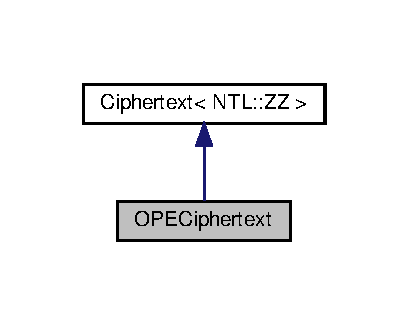
\includegraphics[width=196pt]{classOPECiphertext__inherit__graph}
\end{center}
\end{figure}


Collaboration diagram for O\+P\+E\+Ciphertext\+:
\nopagebreak
\begin{figure}[H]
\begin{center}
\leavevmode
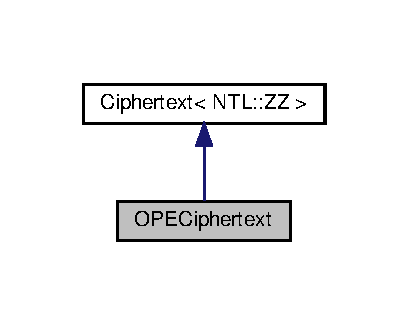
\includegraphics[width=196pt]{classOPECiphertext__coll__graph}
\end{center}
\end{figure}
\subsection*{Public Member Functions}
\begin{DoxyCompactItemize}
\item 
\hyperlink{classOPECiphertext_a03de322445edbdcd1439906f2d853dd0}{O\+P\+E\+Ciphertext} ()
\item 
\hyperlink{classOPECiphertext_a834af7de55af1ba2bb9621099dea4fa7}{O\+P\+E\+Ciphertext} (N\+T\+L\+::\+ZZ \&a)
\item 
\hyperlink{classOPECiphertext_af47076c8c0eb9cdccd0d3ad50140183d}{O\+P\+E\+Ciphertext} (N\+T\+L\+::vec\+\_\+\+ZZ \&a)
\item 
\hyperlink{classOPECiphertext_a8ec336e22de5f54c7dfbe5e4e82b7577}{O\+P\+E\+Ciphertext} (std\+::string \&str)
\item 
virtual \hyperlink{classOPECiphertext_a80e3d4bd7823830c1a26943e6a4959f9}{$\sim$\+O\+P\+E\+Ciphertext} ()
\end{DoxyCompactItemize}
\subsection*{Private Member Functions}
\begin{DoxyCompactItemize}
\item 
{\footnotesize template$<$class Archive $>$ }\\void \hyperlink{classOPECiphertext_a30351d3dd1b2ed7be3bd27abb0180784}{serialize} (Archive \&ar, const unsigned int version)
\end{DoxyCompactItemize}
\subsection*{Friends}
\begin{DoxyCompactItemize}
\item 
class \hyperlink{classOPECiphertext_ac98d07dd8f7b70e16ccb9a01abf56b9c}{boost\+::serialization\+::access}
\item 
std\+::ostream \& \hyperlink{classOPECiphertext_acbdbfe3a8b342ed91b375a30c19423a3}{operator$<$$<$} (std\+::ostream \&o, const \hyperlink{classOPECiphertext}{O\+P\+E\+Ciphertext} \&c)
\item 
std\+::istream \& \hyperlink{classOPECiphertext_a78faeb1ac9b11d0aa4337957b9fba288}{operator$>$$>$} (std\+::istream \&i, \hyperlink{classOPECiphertext}{O\+P\+E\+Ciphertext} \&c)
\item 
bool \hyperlink{classOPECiphertext_a7a856f70b6a7c9c384e5bcc59d4665ca}{operator$<$} (const \hyperlink{classOPECiphertext}{O\+P\+E\+Ciphertext} \&a, const \hyperlink{classOPECiphertext}{O\+P\+E\+Ciphertext} \&b)
\item 
bool \hyperlink{classOPECiphertext_a6e3f45959b24805b5e007867bde5ac52}{operator$<$=} (const \hyperlink{classOPECiphertext}{O\+P\+E\+Ciphertext} \&a, const \hyperlink{classOPECiphertext}{O\+P\+E\+Ciphertext} \&b)
\item 
bool \hyperlink{classOPECiphertext_a434a85cf1acb2e87f59cb598aa67aac1}{operator==} (const \hyperlink{classOPECiphertext}{O\+P\+E\+Ciphertext} \&a, const \hyperlink{classOPECiphertext}{O\+P\+E\+Ciphertext} \&b)
\item 
bool \hyperlink{classOPECiphertext_a5a05c9bf39f65f099132a4cb3c030fc0}{operator$>$} (const \hyperlink{classOPECiphertext}{O\+P\+E\+Ciphertext} \&a, const \hyperlink{classOPECiphertext}{O\+P\+E\+Ciphertext} \&b)
\item 
bool \hyperlink{classOPECiphertext_a2e7887e9daea66096a9526a493cdc023}{operator$>$=} (const \hyperlink{classOPECiphertext}{O\+P\+E\+Ciphertext} \&a, const \hyperlink{classOPECiphertext}{O\+P\+E\+Ciphertext} \&b)
\end{DoxyCompactItemize}
\subsection*{Additional Inherited Members}


\subsection{Constructor \& Destructor Documentation}
\mbox{\Hypertarget{classOPECiphertext_a03de322445edbdcd1439906f2d853dd0}\label{classOPECiphertext_a03de322445edbdcd1439906f2d853dd0}} 
\index{O\+P\+E\+Ciphertext@{O\+P\+E\+Ciphertext}!O\+P\+E\+Ciphertext@{O\+P\+E\+Ciphertext}}
\index{O\+P\+E\+Ciphertext@{O\+P\+E\+Ciphertext}!O\+P\+E\+Ciphertext@{O\+P\+E\+Ciphertext}}
\subsubsection{\texorpdfstring{O\+P\+E\+Ciphertext()}{OPECiphertext()}\hspace{0.1cm}{\footnotesize\ttfamily [1/4]}}
{\footnotesize\ttfamily O\+P\+E\+Ciphertext\+::\+O\+P\+E\+Ciphertext (\begin{DoxyParamCaption}{ }\end{DoxyParamCaption})}

Default constructor \mbox{\Hypertarget{classOPECiphertext_a834af7de55af1ba2bb9621099dea4fa7}\label{classOPECiphertext_a834af7de55af1ba2bb9621099dea4fa7}} 
\index{O\+P\+E\+Ciphertext@{O\+P\+E\+Ciphertext}!O\+P\+E\+Ciphertext@{O\+P\+E\+Ciphertext}}
\index{O\+P\+E\+Ciphertext@{O\+P\+E\+Ciphertext}!O\+P\+E\+Ciphertext@{O\+P\+E\+Ciphertext}}
\subsubsection{\texorpdfstring{O\+P\+E\+Ciphertext()}{OPECiphertext()}\hspace{0.1cm}{\footnotesize\ttfamily [2/4]}}
{\footnotesize\ttfamily O\+P\+E\+Ciphertext\+::\+O\+P\+E\+Ciphertext (\begin{DoxyParamCaption}\item[{N\+T\+L\+::\+ZZ \&}]{a }\end{DoxyParamCaption})}

Initialise {\ttfamily ciphertext} to the value supplied 
\begin{DoxyParams}{Parameters}
{\em a} & An N\+TL multiprecision integer \\
\hline
\end{DoxyParams}
\mbox{\Hypertarget{classOPECiphertext_af47076c8c0eb9cdccd0d3ad50140183d}\label{classOPECiphertext_af47076c8c0eb9cdccd0d3ad50140183d}} 
\index{O\+P\+E\+Ciphertext@{O\+P\+E\+Ciphertext}!O\+P\+E\+Ciphertext@{O\+P\+E\+Ciphertext}}
\index{O\+P\+E\+Ciphertext@{O\+P\+E\+Ciphertext}!O\+P\+E\+Ciphertext@{O\+P\+E\+Ciphertext}}
\subsubsection{\texorpdfstring{O\+P\+E\+Ciphertext()}{OPECiphertext()}\hspace{0.1cm}{\footnotesize\ttfamily [3/4]}}
{\footnotesize\ttfamily O\+P\+E\+Ciphertext\+::\+O\+P\+E\+Ciphertext (\begin{DoxyParamCaption}\item[{N\+T\+L\+::vec\+\_\+\+ZZ \&}]{a }\end{DoxyParamCaption})}

\mbox{\Hypertarget{classOPECiphertext_a8ec336e22de5f54c7dfbe5e4e82b7577}\label{classOPECiphertext_a8ec336e22de5f54c7dfbe5e4e82b7577}} 
\index{O\+P\+E\+Ciphertext@{O\+P\+E\+Ciphertext}!O\+P\+E\+Ciphertext@{O\+P\+E\+Ciphertext}}
\index{O\+P\+E\+Ciphertext@{O\+P\+E\+Ciphertext}!O\+P\+E\+Ciphertext@{O\+P\+E\+Ciphertext}}
\subsubsection{\texorpdfstring{O\+P\+E\+Ciphertext()}{OPECiphertext()}\hspace{0.1cm}{\footnotesize\ttfamily [4/4]}}
{\footnotesize\ttfamily O\+P\+E\+Ciphertext\+::\+O\+P\+E\+Ciphertext (\begin{DoxyParamCaption}\item[{std\+::string \&}]{str }\end{DoxyParamCaption})}

Initialise {\ttfamily ciphertext} to the value supplied 
\begin{DoxyParams}{Parameters}
{\em str} & A decimal string \\
\hline
\end{DoxyParams}
\mbox{\Hypertarget{classOPECiphertext_a80e3d4bd7823830c1a26943e6a4959f9}\label{classOPECiphertext_a80e3d4bd7823830c1a26943e6a4959f9}} 
\index{O\+P\+E\+Ciphertext@{O\+P\+E\+Ciphertext}!````~O\+P\+E\+Ciphertext@{$\sim$\+O\+P\+E\+Ciphertext}}
\index{````~O\+P\+E\+Ciphertext@{$\sim$\+O\+P\+E\+Ciphertext}!O\+P\+E\+Ciphertext@{O\+P\+E\+Ciphertext}}
\subsubsection{\texorpdfstring{$\sim$\+O\+P\+E\+Ciphertext()}{~OPECiphertext()}}
{\footnotesize\ttfamily O\+P\+E\+Ciphertext\+::$\sim$\+O\+P\+E\+Ciphertext (\begin{DoxyParamCaption}{ }\end{DoxyParamCaption})\hspace{0.3cm}{\ttfamily [virtual]}}

Default destructor 

\subsection{Member Function Documentation}
\mbox{\Hypertarget{classOPECiphertext_a30351d3dd1b2ed7be3bd27abb0180784}\label{classOPECiphertext_a30351d3dd1b2ed7be3bd27abb0180784}} 
\index{O\+P\+E\+Ciphertext@{O\+P\+E\+Ciphertext}!serialize@{serialize}}
\index{serialize@{serialize}!O\+P\+E\+Ciphertext@{O\+P\+E\+Ciphertext}}
\subsubsection{\texorpdfstring{serialize()}{serialize()}}
{\footnotesize\ttfamily template$<$class Archive $>$ \\
void O\+P\+E\+Ciphertext\+::serialize (\begin{DoxyParamCaption}\item[{Archive \&}]{ar,  }\item[{const unsigned int}]{version }\end{DoxyParamCaption})\hspace{0.3cm}{\ttfamily [inline]}, {\ttfamily [private]}}



\subsection{Friends And Related Function Documentation}
\mbox{\Hypertarget{classOPECiphertext_ac98d07dd8f7b70e16ccb9a01abf56b9c}\label{classOPECiphertext_ac98d07dd8f7b70e16ccb9a01abf56b9c}} 
\index{O\+P\+E\+Ciphertext@{O\+P\+E\+Ciphertext}!boost\+::serialization\+::access@{boost\+::serialization\+::access}}
\index{boost\+::serialization\+::access@{boost\+::serialization\+::access}!O\+P\+E\+Ciphertext@{O\+P\+E\+Ciphertext}}
\subsubsection{\texorpdfstring{boost\+::serialization\+::access}{boost::serialization::access}}
{\footnotesize\ttfamily friend class boost\+::serialization\+::access\hspace{0.3cm}{\ttfamily [friend]}}

\mbox{\Hypertarget{classOPECiphertext_a7a856f70b6a7c9c384e5bcc59d4665ca}\label{classOPECiphertext_a7a856f70b6a7c9c384e5bcc59d4665ca}} 
\index{O\+P\+E\+Ciphertext@{O\+P\+E\+Ciphertext}!operator$<$@{operator$<$}}
\index{operator$<$@{operator$<$}!O\+P\+E\+Ciphertext@{O\+P\+E\+Ciphertext}}
\subsubsection{\texorpdfstring{operator$<$}{operator<}}
{\footnotesize\ttfamily bool operator$<$ (\begin{DoxyParamCaption}\item[{const \hyperlink{classOPECiphertext}{O\+P\+E\+Ciphertext} \&}]{a,  }\item[{const \hyperlink{classOPECiphertext}{O\+P\+E\+Ciphertext} \&}]{b }\end{DoxyParamCaption})\hspace{0.3cm}{\ttfamily [friend]}}

Returns {\ttfamily a.\+ciphertext} $<$ {\ttfamily b.\+ciphertext} 
\begin{DoxyParams}{Parameters}
{\em a} & {\ttfamily \hyperlink{classOPECiphertext}{O\+P\+E\+Ciphertext}} object \\
\hline
{\em b} & {\ttfamily \hyperlink{classOPECiphertext}{O\+P\+E\+Ciphertext}} object \\
\hline
\end{DoxyParams}
\begin{DoxyReturn}{Returns}
{\ttfamily true} or {\ttfamily false} 
\end{DoxyReturn}
\mbox{\Hypertarget{classOPECiphertext_acbdbfe3a8b342ed91b375a30c19423a3}\label{classOPECiphertext_acbdbfe3a8b342ed91b375a30c19423a3}} 
\index{O\+P\+E\+Ciphertext@{O\+P\+E\+Ciphertext}!operator$<$$<$@{operator$<$$<$}}
\index{operator$<$$<$@{operator$<$$<$}!O\+P\+E\+Ciphertext@{O\+P\+E\+Ciphertext}}
\subsubsection{\texorpdfstring{operator$<$$<$}{operator<<}}
{\footnotesize\ttfamily std\+::ostream\& operator$<$$<$ (\begin{DoxyParamCaption}\item[{std\+::ostream \&}]{o,  }\item[{const \hyperlink{classOPECiphertext}{O\+P\+E\+Ciphertext} \&}]{c }\end{DoxyParamCaption})\hspace{0.3cm}{\ttfamily [friend]}}

Write {\ttfamily ciphertext} as decimal string to the output stream 
\begin{DoxyParams}{Parameters}
{\em o} & Output stream \\
\hline
{\em c} & {\ttfamily \hyperlink{classOPECiphertext}{O\+P\+E\+Ciphertext}} object \\
\hline
\end{DoxyParams}
\begin{DoxyReturn}{Returns}
a reference to the output stream 
\end{DoxyReturn}
\mbox{\Hypertarget{classOPECiphertext_a6e3f45959b24805b5e007867bde5ac52}\label{classOPECiphertext_a6e3f45959b24805b5e007867bde5ac52}} 
\index{O\+P\+E\+Ciphertext@{O\+P\+E\+Ciphertext}!operator$<$=@{operator$<$=}}
\index{operator$<$=@{operator$<$=}!O\+P\+E\+Ciphertext@{O\+P\+E\+Ciphertext}}
\subsubsection{\texorpdfstring{operator$<$=}{operator<=}}
{\footnotesize\ttfamily bool operator$<$= (\begin{DoxyParamCaption}\item[{const \hyperlink{classOPECiphertext}{O\+P\+E\+Ciphertext} \&}]{a,  }\item[{const \hyperlink{classOPECiphertext}{O\+P\+E\+Ciphertext} \&}]{b }\end{DoxyParamCaption})\hspace{0.3cm}{\ttfamily [friend]}}

Returns {\ttfamily a.\+ciphertext} {$\le$} {\ttfamily b.\+ciphertext} 
\begin{DoxyParams}{Parameters}
{\em a} & {\ttfamily \hyperlink{classOPECiphertext}{O\+P\+E\+Ciphertext}} object \\
\hline
{\em b} & {\ttfamily \hyperlink{classOPECiphertext}{O\+P\+E\+Ciphertext}} object \\
\hline
\end{DoxyParams}
\begin{DoxyReturn}{Returns}
{\ttfamily true} or {\ttfamily false} 
\end{DoxyReturn}
\mbox{\Hypertarget{classOPECiphertext_a434a85cf1acb2e87f59cb598aa67aac1}\label{classOPECiphertext_a434a85cf1acb2e87f59cb598aa67aac1}} 
\index{O\+P\+E\+Ciphertext@{O\+P\+E\+Ciphertext}!operator==@{operator==}}
\index{operator==@{operator==}!O\+P\+E\+Ciphertext@{O\+P\+E\+Ciphertext}}
\subsubsection{\texorpdfstring{operator==}{operator==}}
{\footnotesize\ttfamily bool operator== (\begin{DoxyParamCaption}\item[{const \hyperlink{classOPECiphertext}{O\+P\+E\+Ciphertext} \&}]{a,  }\item[{const \hyperlink{classOPECiphertext}{O\+P\+E\+Ciphertext} \&}]{b }\end{DoxyParamCaption})\hspace{0.3cm}{\ttfamily [friend]}}

Returns {\ttfamily a.\+ciphertext} = {\ttfamily b.\+ciphertext} 
\begin{DoxyParams}{Parameters}
{\em a} & {\ttfamily \hyperlink{classOPECiphertext}{O\+P\+E\+Ciphertext}} object \\
\hline
{\em b} & {\ttfamily \hyperlink{classOPECiphertext}{O\+P\+E\+Ciphertext}} object \\
\hline
\end{DoxyParams}
\begin{DoxyReturn}{Returns}
{\ttfamily true} or {\ttfamily false} 
\end{DoxyReturn}
\mbox{\Hypertarget{classOPECiphertext_a5a05c9bf39f65f099132a4cb3c030fc0}\label{classOPECiphertext_a5a05c9bf39f65f099132a4cb3c030fc0}} 
\index{O\+P\+E\+Ciphertext@{O\+P\+E\+Ciphertext}!operator$>$@{operator$>$}}
\index{operator$>$@{operator$>$}!O\+P\+E\+Ciphertext@{O\+P\+E\+Ciphertext}}
\subsubsection{\texorpdfstring{operator$>$}{operator>}}
{\footnotesize\ttfamily bool operator$>$ (\begin{DoxyParamCaption}\item[{const \hyperlink{classOPECiphertext}{O\+P\+E\+Ciphertext} \&}]{a,  }\item[{const \hyperlink{classOPECiphertext}{O\+P\+E\+Ciphertext} \&}]{b }\end{DoxyParamCaption})\hspace{0.3cm}{\ttfamily [friend]}}

Returns {\ttfamily a.\+ciphertext} $>$ {\ttfamily b.\+ciphertext} 
\begin{DoxyParams}{Parameters}
{\em a} & {\ttfamily \hyperlink{classOPECiphertext}{O\+P\+E\+Ciphertext}} object \\
\hline
{\em b} & {\ttfamily \hyperlink{classOPECiphertext}{O\+P\+E\+Ciphertext}} object \\
\hline
\end{DoxyParams}
\begin{DoxyReturn}{Returns}
{\ttfamily true} or {\ttfamily false} 
\end{DoxyReturn}
\mbox{\Hypertarget{classOPECiphertext_a2e7887e9daea66096a9526a493cdc023}\label{classOPECiphertext_a2e7887e9daea66096a9526a493cdc023}} 
\index{O\+P\+E\+Ciphertext@{O\+P\+E\+Ciphertext}!operator$>$=@{operator$>$=}}
\index{operator$>$=@{operator$>$=}!O\+P\+E\+Ciphertext@{O\+P\+E\+Ciphertext}}
\subsubsection{\texorpdfstring{operator$>$=}{operator>=}}
{\footnotesize\ttfamily bool operator$>$= (\begin{DoxyParamCaption}\item[{const \hyperlink{classOPECiphertext}{O\+P\+E\+Ciphertext} \&}]{a,  }\item[{const \hyperlink{classOPECiphertext}{O\+P\+E\+Ciphertext} \&}]{b }\end{DoxyParamCaption})\hspace{0.3cm}{\ttfamily [friend]}}

Returns {\ttfamily a.\+ciphertext} {$\ge$} {\ttfamily b.\+ciphertext} 
\begin{DoxyParams}{Parameters}
{\em a} & {\ttfamily \hyperlink{classOPECiphertext}{O\+P\+E\+Ciphertext}} object \\
\hline
{\em b} & {\ttfamily \hyperlink{classOPECiphertext}{O\+P\+E\+Ciphertext}} object \\
\hline
\end{DoxyParams}
\begin{DoxyReturn}{Returns}
{\ttfamily true} or {\ttfamily false} 
\end{DoxyReturn}
\mbox{\Hypertarget{classOPECiphertext_a78faeb1ac9b11d0aa4337957b9fba288}\label{classOPECiphertext_a78faeb1ac9b11d0aa4337957b9fba288}} 
\index{O\+P\+E\+Ciphertext@{O\+P\+E\+Ciphertext}!operator$>$$>$@{operator$>$$>$}}
\index{operator$>$$>$@{operator$>$$>$}!O\+P\+E\+Ciphertext@{O\+P\+E\+Ciphertext}}
\subsubsection{\texorpdfstring{operator$>$$>$}{operator>>}}
{\footnotesize\ttfamily std\+::istream\& operator$>$$>$ (\begin{DoxyParamCaption}\item[{std\+::istream \&}]{i,  }\item[{\hyperlink{classOPECiphertext}{O\+P\+E\+Ciphertext} \&}]{c }\end{DoxyParamCaption})\hspace{0.3cm}{\ttfamily [friend]}}

Read {\ttfamily ciphertext} as decimal string from the input stream and convert to {\ttfamily N\+T\+L\+::\+ZZ} 
\begin{DoxyParams}{Parameters}
{\em i} & Input stream \\
\hline
{\em c} & {\ttfamily \hyperlink{classOPECiphertext}{O\+P\+E\+Ciphertext}} object \\
\hline
\end{DoxyParams}
\begin{DoxyReturn}{Returns}
a reference to the output stream 
\end{DoxyReturn}


The documentation for this class was generated from the following files\+:\begin{DoxyCompactItemize}
\item 
include/\hyperlink{OPECiphertext_8h}{O\+P\+E\+Ciphertext.\+h}\item 
src/\hyperlink{OPECiphertext_8cpp}{O\+P\+E\+Ciphertext.\+cpp}\end{DoxyCompactItemize}

\hypertarget{classPolyCiphertext}{}\section{Poly\+Ciphertext Class Reference}
\label{classPolyCiphertext}\index{Poly\+Ciphertext@{Poly\+Ciphertext}}


{\ttfamily \#include $<$Poly\+Ciphertext.\+h$>$}



Inheritance diagram for Poly\+Ciphertext\+:
\nopagebreak
\begin{figure}[H]
\begin{center}
\leavevmode
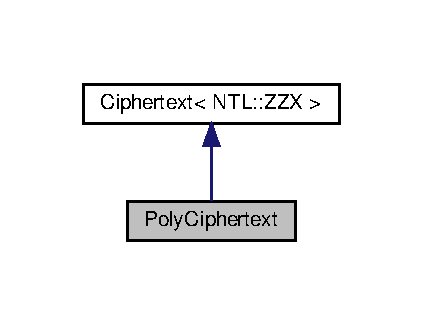
\includegraphics[width=203pt]{classPolyCiphertext__inherit__graph}
\end{center}
\end{figure}


Collaboration diagram for Poly\+Ciphertext\+:
\nopagebreak
\begin{figure}[H]
\begin{center}
\leavevmode
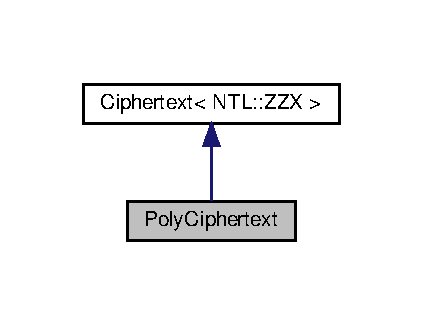
\includegraphics[width=203pt]{classPolyCiphertext__coll__graph}
\end{center}
\end{figure}
\subsection*{Public Member Functions}
\begin{DoxyCompactItemize}
\item 
\hyperlink{classPolyCiphertext_ae081c8472f7ec80bea8793401b605436}{Poly\+Ciphertext} ()
\item 
\hyperlink{classPolyCiphertext_a48360be9981b6b84eb48be372bb3296a}{Poly\+Ciphertext} (N\+T\+L\+::\+Z\+ZX \&a)
\item 
\hyperlink{classPolyCiphertext_a4dc4594b14dee8e42ac35537506fb0fd}{Poly\+Ciphertext} (N\+T\+L\+::vec\+\_\+\+ZZ \&a)
\item 
\hyperlink{classPolyCiphertext_ad46cd9f5dfa2313798e5302f7d7a9445}{Poly\+Ciphertext} (std\+::string \&str)
\item 
virtual \hyperlink{classPolyCiphertext_aeee18e28294a2cac4e95fcc704026673}{$\sim$\+Poly\+Ciphertext} ()
\item 
std\+::string \hyperlink{classPolyCiphertext_a4ffc33808a07305df76a26a0fdc60d8e}{to\+\_\+string} ()
\end{DoxyCompactItemize}
\subsection*{Private Member Functions}
\begin{DoxyCompactItemize}
\item 
{\footnotesize template$<$class Archive $>$ }\\void \hyperlink{classPolyCiphertext_a6405ebc8f6ad048239ea6f8d677702af}{serialize} (Archive \&ar, const unsigned int version)
\end{DoxyCompactItemize}
\subsection*{Friends}
\begin{DoxyCompactItemize}
\item 
class \hyperlink{classPolyCiphertext_ac98d07dd8f7b70e16ccb9a01abf56b9c}{boost\+::serialization\+::access}
\item 
int \hyperlink{classPolyCiphertext_a2a25d0399b812261d703d84fd3a21fb9}{compare} (const \hyperlink{classPolyCiphertext}{Poly\+Ciphertext} \&a, const \hyperlink{classPolyCiphertext}{Poly\+Ciphertext} \&b)
\item 
bool \hyperlink{classPolyCiphertext_ab5a64cd27170239ff233b1a17f5b0de9}{operator$<$} (const \hyperlink{classPolyCiphertext}{Poly\+Ciphertext} \&a, const \hyperlink{classPolyCiphertext}{Poly\+Ciphertext} \&b)
\item 
bool \hyperlink{classPolyCiphertext_a3199ddbed52caee0d591894b60389144}{operator$<$=} (const \hyperlink{classPolyCiphertext}{Poly\+Ciphertext} \&a, const \hyperlink{classPolyCiphertext}{Poly\+Ciphertext} \&b)
\item 
bool \hyperlink{classPolyCiphertext_a441251a147b7c15eccf64048ba9fb0fe}{operator==} (const \hyperlink{classPolyCiphertext}{Poly\+Ciphertext} \&a, const \hyperlink{classPolyCiphertext}{Poly\+Ciphertext} \&b)
\item 
bool \hyperlink{classPolyCiphertext_a2a58b35102feabe6b31bacdd457d7884}{operator$>$} (const \hyperlink{classPolyCiphertext}{Poly\+Ciphertext} \&a, const \hyperlink{classPolyCiphertext}{Poly\+Ciphertext} \&b)
\item 
bool \hyperlink{classPolyCiphertext_ab76ec0162c70ea00a11f921d617d102d}{operator$>$=} (const \hyperlink{classPolyCiphertext}{Poly\+Ciphertext} \&a, const \hyperlink{classPolyCiphertext}{Poly\+Ciphertext} \&b)
\end{DoxyCompactItemize}
\subsection*{Additional Inherited Members}


\subsection{Constructor \& Destructor Documentation}
\mbox{\Hypertarget{classPolyCiphertext_ae081c8472f7ec80bea8793401b605436}\label{classPolyCiphertext_ae081c8472f7ec80bea8793401b605436}} 
\index{Poly\+Ciphertext@{Poly\+Ciphertext}!Poly\+Ciphertext@{Poly\+Ciphertext}}
\index{Poly\+Ciphertext@{Poly\+Ciphertext}!Poly\+Ciphertext@{Poly\+Ciphertext}}
\subsubsection{\texorpdfstring{Poly\+Ciphertext()}{PolyCiphertext()}\hspace{0.1cm}{\footnotesize\ttfamily [1/4]}}
{\footnotesize\ttfamily Poly\+Ciphertext\+::\+Poly\+Ciphertext (\begin{DoxyParamCaption}{ }\end{DoxyParamCaption})}

Default constructor \mbox{\Hypertarget{classPolyCiphertext_a48360be9981b6b84eb48be372bb3296a}\label{classPolyCiphertext_a48360be9981b6b84eb48be372bb3296a}} 
\index{Poly\+Ciphertext@{Poly\+Ciphertext}!Poly\+Ciphertext@{Poly\+Ciphertext}}
\index{Poly\+Ciphertext@{Poly\+Ciphertext}!Poly\+Ciphertext@{Poly\+Ciphertext}}
\subsubsection{\texorpdfstring{Poly\+Ciphertext()}{PolyCiphertext()}\hspace{0.1cm}{\footnotesize\ttfamily [2/4]}}
{\footnotesize\ttfamily Poly\+Ciphertext\+::\+Poly\+Ciphertext (\begin{DoxyParamCaption}\item[{N\+T\+L\+::\+Z\+ZX \&}]{a }\end{DoxyParamCaption})}

Initialises the ciphertext with {\ttfamily a} 
\begin{DoxyParams}{Parameters}
{\em a} & An N\+TL representation of a Z\mbox{[}x\mbox{]} polynomial \\
\hline
\end{DoxyParams}
\mbox{\Hypertarget{classPolyCiphertext_a4dc4594b14dee8e42ac35537506fb0fd}\label{classPolyCiphertext_a4dc4594b14dee8e42ac35537506fb0fd}} 
\index{Poly\+Ciphertext@{Poly\+Ciphertext}!Poly\+Ciphertext@{Poly\+Ciphertext}}
\index{Poly\+Ciphertext@{Poly\+Ciphertext}!Poly\+Ciphertext@{Poly\+Ciphertext}}
\subsubsection{\texorpdfstring{Poly\+Ciphertext()}{PolyCiphertext()}\hspace{0.1cm}{\footnotesize\ttfamily [3/4]}}
{\footnotesize\ttfamily Poly\+Ciphertext\+::\+Poly\+Ciphertext (\begin{DoxyParamCaption}\item[{N\+T\+L\+::vec\+\_\+\+ZZ \&}]{a }\end{DoxyParamCaption})}

Intialises the ciphertext as a degree zero polynomial (constant) with value {\ttfamily a} 
\begin{DoxyParams}{Parameters}
{\em a} & \\
\hline
\end{DoxyParams}
\mbox{\Hypertarget{classPolyCiphertext_ad46cd9f5dfa2313798e5302f7d7a9445}\label{classPolyCiphertext_ad46cd9f5dfa2313798e5302f7d7a9445}} 
\index{Poly\+Ciphertext@{Poly\+Ciphertext}!Poly\+Ciphertext@{Poly\+Ciphertext}}
\index{Poly\+Ciphertext@{Poly\+Ciphertext}!Poly\+Ciphertext@{Poly\+Ciphertext}}
\subsubsection{\texorpdfstring{Poly\+Ciphertext()}{PolyCiphertext()}\hspace{0.1cm}{\footnotesize\ttfamily [4/4]}}
{\footnotesize\ttfamily Poly\+Ciphertext\+::\+Poly\+Ciphertext (\begin{DoxyParamCaption}\item[{std\+::string \&}]{str }\end{DoxyParamCaption})}

Initialises the ciphertext using the string representation of the polynomial from {\ttfamily str} 
\begin{DoxyParams}{Parameters}
{\em str} & \\
\hline
\end{DoxyParams}
\mbox{\Hypertarget{classPolyCiphertext_aeee18e28294a2cac4e95fcc704026673}\label{classPolyCiphertext_aeee18e28294a2cac4e95fcc704026673}} 
\index{Poly\+Ciphertext@{Poly\+Ciphertext}!````~Poly\+Ciphertext@{$\sim$\+Poly\+Ciphertext}}
\index{````~Poly\+Ciphertext@{$\sim$\+Poly\+Ciphertext}!Poly\+Ciphertext@{Poly\+Ciphertext}}
\subsubsection{\texorpdfstring{$\sim$\+Poly\+Ciphertext()}{~PolyCiphertext()}}
{\footnotesize\ttfamily Poly\+Ciphertext\+::$\sim$\+Poly\+Ciphertext (\begin{DoxyParamCaption}{ }\end{DoxyParamCaption})\hspace{0.3cm}{\ttfamily [virtual]}}

Default destructor 

\subsection{Member Function Documentation}
\mbox{\Hypertarget{classPolyCiphertext_a6405ebc8f6ad048239ea6f8d677702af}\label{classPolyCiphertext_a6405ebc8f6ad048239ea6f8d677702af}} 
\index{Poly\+Ciphertext@{Poly\+Ciphertext}!serialize@{serialize}}
\index{serialize@{serialize}!Poly\+Ciphertext@{Poly\+Ciphertext}}
\subsubsection{\texorpdfstring{serialize()}{serialize()}}
{\footnotesize\ttfamily template$<$class Archive $>$ \\
void Poly\+Ciphertext\+::serialize (\begin{DoxyParamCaption}\item[{Archive \&}]{ar,  }\item[{const unsigned int}]{version }\end{DoxyParamCaption})\hspace{0.3cm}{\ttfamily [inline]}, {\ttfamily [private]}}

\mbox{\Hypertarget{classPolyCiphertext_a4ffc33808a07305df76a26a0fdc60d8e}\label{classPolyCiphertext_a4ffc33808a07305df76a26a0fdc60d8e}} 
\index{Poly\+Ciphertext@{Poly\+Ciphertext}!to\+\_\+string@{to\+\_\+string}}
\index{to\+\_\+string@{to\+\_\+string}!Poly\+Ciphertext@{Poly\+Ciphertext}}
\subsubsection{\texorpdfstring{to\+\_\+string()}{to\_string()}}
{\footnotesize\ttfamily std\+::string Poly\+Ciphertext\+::to\+\_\+string (\begin{DoxyParamCaption}{ }\end{DoxyParamCaption})}

Write polynomial to a string. The string is a space separated list of the coefficients enclosed by square brackets. \begin{DoxyReturn}{Returns}
String respresentation of the polynomials 
\end{DoxyReturn}


\subsection{Friends And Related Function Documentation}
\mbox{\Hypertarget{classPolyCiphertext_ac98d07dd8f7b70e16ccb9a01abf56b9c}\label{classPolyCiphertext_ac98d07dd8f7b70e16ccb9a01abf56b9c}} 
\index{Poly\+Ciphertext@{Poly\+Ciphertext}!boost\+::serialization\+::access@{boost\+::serialization\+::access}}
\index{boost\+::serialization\+::access@{boost\+::serialization\+::access}!Poly\+Ciphertext@{Poly\+Ciphertext}}
\subsubsection{\texorpdfstring{boost\+::serialization\+::access}{boost::serialization::access}}
{\footnotesize\ttfamily friend class boost\+::serialization\+::access\hspace{0.3cm}{\ttfamily [friend]}}

\mbox{\Hypertarget{classPolyCiphertext_a2a25d0399b812261d703d84fd3a21fb9}\label{classPolyCiphertext_a2a25d0399b812261d703d84fd3a21fb9}} 
\index{Poly\+Ciphertext@{Poly\+Ciphertext}!compare@{compare}}
\index{compare@{compare}!Poly\+Ciphertext@{Poly\+Ciphertext}}
\subsubsection{\texorpdfstring{compare}{compare}}
{\footnotesize\ttfamily int compare (\begin{DoxyParamCaption}\item[{const \hyperlink{classPolyCiphertext}{Poly\+Ciphertext} \&}]{a,  }\item[{const \hyperlink{classPolyCiphertext}{Poly\+Ciphertext} \&}]{b }\end{DoxyParamCaption})\hspace{0.3cm}{\ttfamily [friend]}}

Auxiliary function to compare two polynomials lexicographically (a polynomial of larger degree is considered to be ordered higher than a lower degree polynomial). Returns -\/1 is {\ttfamily a.\+ciphertext} $<$ {\ttfamily b.\+ciphertext}, 0 if {\ttfamily a.\+ciphertext} = {\ttfamily b.\+ciphertext}, and 1 if {\ttfamily a.\+ciphertext} $>$ {\ttfamily b.\+ciphertext} 
\begin{DoxyParams}{Parameters}
{\em a} & A {\ttfamily \hyperlink{classPolyCiphertext}{Poly\+Ciphertext}} object \\
\hline
{\em b} & A {\ttfamily \hyperlink{classPolyCiphertext}{Poly\+Ciphertext}} object \\
\hline
\end{DoxyParams}
\begin{DoxyReturn}{Returns}
-\/1, 0, or 1 
\end{DoxyReturn}
\mbox{\Hypertarget{classPolyCiphertext_ab5a64cd27170239ff233b1a17f5b0de9}\label{classPolyCiphertext_ab5a64cd27170239ff233b1a17f5b0de9}} 
\index{Poly\+Ciphertext@{Poly\+Ciphertext}!operator$<$@{operator$<$}}
\index{operator$<$@{operator$<$}!Poly\+Ciphertext@{Poly\+Ciphertext}}
\subsubsection{\texorpdfstring{operator$<$}{operator<}}
{\footnotesize\ttfamily bool operator$<$ (\begin{DoxyParamCaption}\item[{const \hyperlink{classPolyCiphertext}{Poly\+Ciphertext} \&}]{a,  }\item[{const \hyperlink{classPolyCiphertext}{Poly\+Ciphertext} \&}]{b }\end{DoxyParamCaption})\hspace{0.3cm}{\ttfamily [friend]}}

Returns true if {\ttfamily a.\+ciphertext} is strictly less than {\ttfamily b.\+ciphertext} 
\begin{DoxyParams}{Parameters}
{\em a} & A {\ttfamily \hyperlink{classPolyCiphertext}{Poly\+Ciphertext}} object \\
\hline
{\em b} & A {\ttfamily \hyperlink{classPolyCiphertext}{Poly\+Ciphertext}} object \\
\hline
\end{DoxyParams}
\begin{DoxyReturn}{Returns}
{\ttfamily true} or {\ttfamily false} 
\end{DoxyReturn}
\mbox{\Hypertarget{classPolyCiphertext_a3199ddbed52caee0d591894b60389144}\label{classPolyCiphertext_a3199ddbed52caee0d591894b60389144}} 
\index{Poly\+Ciphertext@{Poly\+Ciphertext}!operator$<$=@{operator$<$=}}
\index{operator$<$=@{operator$<$=}!Poly\+Ciphertext@{Poly\+Ciphertext}}
\subsubsection{\texorpdfstring{operator$<$=}{operator<=}}
{\footnotesize\ttfamily bool operator$<$= (\begin{DoxyParamCaption}\item[{const \hyperlink{classPolyCiphertext}{Poly\+Ciphertext} \&}]{a,  }\item[{const \hyperlink{classPolyCiphertext}{Poly\+Ciphertext} \&}]{b }\end{DoxyParamCaption})\hspace{0.3cm}{\ttfamily [friend]}}

Returns true if {\ttfamily a.\+ciphertext} is less than or equal to {\ttfamily b.\+ciphertext} 
\begin{DoxyParams}{Parameters}
{\em a} & A {\ttfamily \hyperlink{classPolyCiphertext}{Poly\+Ciphertext}} object \\
\hline
{\em b} & A {\ttfamily \hyperlink{classPolyCiphertext}{Poly\+Ciphertext}} object \\
\hline
\end{DoxyParams}
\begin{DoxyReturn}{Returns}
{\ttfamily true} or {\ttfamily false} 
\end{DoxyReturn}
\mbox{\Hypertarget{classPolyCiphertext_a441251a147b7c15eccf64048ba9fb0fe}\label{classPolyCiphertext_a441251a147b7c15eccf64048ba9fb0fe}} 
\index{Poly\+Ciphertext@{Poly\+Ciphertext}!operator==@{operator==}}
\index{operator==@{operator==}!Poly\+Ciphertext@{Poly\+Ciphertext}}
\subsubsection{\texorpdfstring{operator==}{operator==}}
{\footnotesize\ttfamily bool operator== (\begin{DoxyParamCaption}\item[{const \hyperlink{classPolyCiphertext}{Poly\+Ciphertext} \&}]{a,  }\item[{const \hyperlink{classPolyCiphertext}{Poly\+Ciphertext} \&}]{b }\end{DoxyParamCaption})\hspace{0.3cm}{\ttfamily [friend]}}

Returns true if {\ttfamily a.\+ciphertext} is equal to {\ttfamily b.\+ciphertext} 
\begin{DoxyParams}{Parameters}
{\em a} & A {\ttfamily \hyperlink{classPolyCiphertext}{Poly\+Ciphertext}} object \\
\hline
{\em b} & A {\ttfamily \hyperlink{classPolyCiphertext}{Poly\+Ciphertext}} object \\
\hline
\end{DoxyParams}
\begin{DoxyReturn}{Returns}
{\ttfamily true} or {\ttfamily false} 
\end{DoxyReturn}
\mbox{\Hypertarget{classPolyCiphertext_a2a58b35102feabe6b31bacdd457d7884}\label{classPolyCiphertext_a2a58b35102feabe6b31bacdd457d7884}} 
\index{Poly\+Ciphertext@{Poly\+Ciphertext}!operator$>$@{operator$>$}}
\index{operator$>$@{operator$>$}!Poly\+Ciphertext@{Poly\+Ciphertext}}
\subsubsection{\texorpdfstring{operator$>$}{operator>}}
{\footnotesize\ttfamily bool operator$>$ (\begin{DoxyParamCaption}\item[{const \hyperlink{classPolyCiphertext}{Poly\+Ciphertext} \&}]{a,  }\item[{const \hyperlink{classPolyCiphertext}{Poly\+Ciphertext} \&}]{b }\end{DoxyParamCaption})\hspace{0.3cm}{\ttfamily [friend]}}

Returns true if {\ttfamily a.\+ciphertext} is greater than {\ttfamily b.\+ciphertext} 
\begin{DoxyParams}{Parameters}
{\em a} & A {\ttfamily \hyperlink{classPolyCiphertext}{Poly\+Ciphertext}} object \\
\hline
{\em b} & A {\ttfamily \hyperlink{classPolyCiphertext}{Poly\+Ciphertext}} object \\
\hline
\end{DoxyParams}
\begin{DoxyReturn}{Returns}
{\ttfamily true} or {\ttfamily false} 
\end{DoxyReturn}
\mbox{\Hypertarget{classPolyCiphertext_ab76ec0162c70ea00a11f921d617d102d}\label{classPolyCiphertext_ab76ec0162c70ea00a11f921d617d102d}} 
\index{Poly\+Ciphertext@{Poly\+Ciphertext}!operator$>$=@{operator$>$=}}
\index{operator$>$=@{operator$>$=}!Poly\+Ciphertext@{Poly\+Ciphertext}}
\subsubsection{\texorpdfstring{operator$>$=}{operator>=}}
{\footnotesize\ttfamily bool operator$>$= (\begin{DoxyParamCaption}\item[{const \hyperlink{classPolyCiphertext}{Poly\+Ciphertext} \&}]{a,  }\item[{const \hyperlink{classPolyCiphertext}{Poly\+Ciphertext} \&}]{b }\end{DoxyParamCaption})\hspace{0.3cm}{\ttfamily [friend]}}

Returns true if {\ttfamily a.\+ciphertext} is greater than or equal to {\ttfamily b.\+ciphertext} 
\begin{DoxyParams}{Parameters}
{\em a} & A {\ttfamily \hyperlink{classPolyCiphertext}{Poly\+Ciphertext}} object \\
\hline
{\em b} & A {\ttfamily \hyperlink{classPolyCiphertext}{Poly\+Ciphertext}} object \\
\hline
\end{DoxyParams}
\begin{DoxyReturn}{Returns}
{\ttfamily true} or {\ttfamily false} 
\end{DoxyReturn}


The documentation for this class was generated from the following files\+:\begin{DoxyCompactItemize}
\item 
include/\hyperlink{PolyCiphertext_8h}{Poly\+Ciphertext.\+h}\item 
src/\hyperlink{PolyCiphertext_8cpp}{Poly\+Ciphertext.\+cpp}\end{DoxyCompactItemize}

\hypertarget{classSSECiphertext}{}\section{S\+S\+E\+Ciphertext Class Reference}
\label{classSSECiphertext}\index{S\+S\+E\+Ciphertext@{S\+S\+E\+Ciphertext}}


{\ttfamily \#include $<$S\+S\+E\+Ciphertext.\+h$>$}



Inheritance diagram for S\+S\+E\+Ciphertext\+:
\nopagebreak
\begin{figure}[H]
\begin{center}
\leavevmode
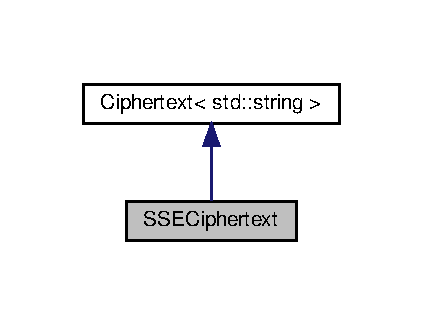
\includegraphics[width=203pt]{classSSECiphertext__inherit__graph}
\end{center}
\end{figure}


Collaboration diagram for S\+S\+E\+Ciphertext\+:
\nopagebreak
\begin{figure}[H]
\begin{center}
\leavevmode
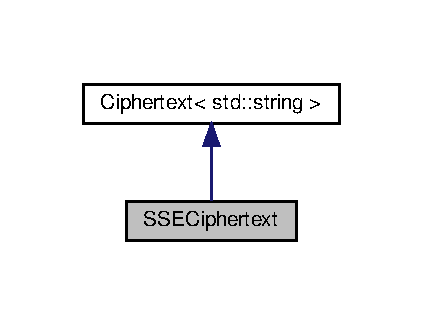
\includegraphics[width=203pt]{classSSECiphertext__coll__graph}
\end{center}
\end{figure}
\subsection*{Public Member Functions}
\begin{DoxyCompactItemize}
\item 
\hyperlink{classSSECiphertext_af8584c9ba9fa27ff1c517fcbea5e0c23}{S\+S\+E\+Ciphertext} ()
\item 
\hyperlink{classSSECiphertext_a77d3038e752e8ba2bca49361c422142f}{S\+S\+E\+Ciphertext} (std\+::string \&\hyperlink{classCiphertext_adef9aae9d923eb100b4a1ad58ce495f1}{ciphertext})
\item 
virtual \hyperlink{classSSECiphertext_a430e67e5f6deef79141accf4dc243ea4}{$\sim$\+S\+S\+E\+Ciphertext} ()
\item 
bool \hyperlink{classSSECiphertext_ac306ffad97bf6ee7093e0ca7f3929222}{match} (std\+::string \&hex\+Encoded\+Key)
\item 
bool \hyperlink{classSSECiphertext_abc37153050ef9bbf76638dd3c64c8a16}{match} (Crypto\+P\+P\+::\+Sec\+Byte\+Block \&key)
\end{DoxyCompactItemize}
\subsection*{Private Member Functions}
\begin{DoxyCompactItemize}
\item 
Crypto\+P\+P\+::\+Sec\+Byte\+Block \hyperlink{classSSECiphertext_af3a871206735d627f7fe7761097d307b}{decode\+Hex\+String} (std\+::string \&hex\+String)
\item 
{\footnotesize template$<$class Archive $>$ }\\void \hyperlink{classSSECiphertext_a8ef115f04a88ca1bc4e4e5ef619f5c93}{serialize} (Archive \&ar, const unsigned int version)
\end{DoxyCompactItemize}
\subsection*{Private Attributes}
\begin{DoxyCompactItemize}
\item 
Crypto\+P\+P\+::\+Sec\+Byte\+Block \hyperlink{classSSECiphertext_a22682a68ecf569e219173c6955c4403e}{tag}
\item 
Crypto\+P\+P\+::\+Sec\+Byte\+Block \hyperlink{classSSECiphertext_a90eed1ea5ce709cac4d57eb9f7ba77aa}{payload}
\item 
Crypto\+P\+P\+::\+C\+M\+AC$<$ Crypto\+P\+P\+::\+A\+ES $>$ \hyperlink{classSSECiphertext_ab2c817fd8b33aef10acf723a00c19507}{mac}
\end{DoxyCompactItemize}
\subsection*{Friends}
\begin{DoxyCompactItemize}
\item 
class \hyperlink{classSSECiphertext_ac98d07dd8f7b70e16ccb9a01abf56b9c}{boost\+::serialization\+::access}
\end{DoxyCompactItemize}
\subsection*{Additional Inherited Members}


\subsection{Constructor \& Destructor Documentation}
\mbox{\Hypertarget{classSSECiphertext_af8584c9ba9fa27ff1c517fcbea5e0c23}\label{classSSECiphertext_af8584c9ba9fa27ff1c517fcbea5e0c23}} 
\index{S\+S\+E\+Ciphertext@{S\+S\+E\+Ciphertext}!S\+S\+E\+Ciphertext@{S\+S\+E\+Ciphertext}}
\index{S\+S\+E\+Ciphertext@{S\+S\+E\+Ciphertext}!S\+S\+E\+Ciphertext@{S\+S\+E\+Ciphertext}}
\subsubsection{\texorpdfstring{S\+S\+E\+Ciphertext()}{SSECiphertext()}\hspace{0.1cm}{\footnotesize\ttfamily [1/2]}}
{\footnotesize\ttfamily S\+S\+E\+Ciphertext\+::\+S\+S\+E\+Ciphertext (\begin{DoxyParamCaption}{ }\end{DoxyParamCaption})}

Default constructor. Required for {\ttfamily boost} serialization. \mbox{\Hypertarget{classSSECiphertext_a77d3038e752e8ba2bca49361c422142f}\label{classSSECiphertext_a77d3038e752e8ba2bca49361c422142f}} 
\index{S\+S\+E\+Ciphertext@{S\+S\+E\+Ciphertext}!S\+S\+E\+Ciphertext@{S\+S\+E\+Ciphertext}}
\index{S\+S\+E\+Ciphertext@{S\+S\+E\+Ciphertext}!S\+S\+E\+Ciphertext@{S\+S\+E\+Ciphertext}}
\subsubsection{\texorpdfstring{S\+S\+E\+Ciphertext()}{SSECiphertext()}\hspace{0.1cm}{\footnotesize\ttfamily [2/2]}}
{\footnotesize\ttfamily S\+S\+E\+Ciphertext\+::\+S\+S\+E\+Ciphertext (\begin{DoxyParamCaption}\item[{std\+::string \&}]{ciphertext }\end{DoxyParamCaption})}

Intialises class members from the J\+S\+ON string supplied as an argument 
\begin{DoxyParams}{Parameters}
{\em ciphertext} & J\+S\+ON string \\
\hline
\end{DoxyParams}
\mbox{\Hypertarget{classSSECiphertext_a430e67e5f6deef79141accf4dc243ea4}\label{classSSECiphertext_a430e67e5f6deef79141accf4dc243ea4}} 
\index{S\+S\+E\+Ciphertext@{S\+S\+E\+Ciphertext}!````~S\+S\+E\+Ciphertext@{$\sim$\+S\+S\+E\+Ciphertext}}
\index{````~S\+S\+E\+Ciphertext@{$\sim$\+S\+S\+E\+Ciphertext}!S\+S\+E\+Ciphertext@{S\+S\+E\+Ciphertext}}
\subsubsection{\texorpdfstring{$\sim$\+S\+S\+E\+Ciphertext()}{~SSECiphertext()}}
{\footnotesize\ttfamily S\+S\+E\+Ciphertext\+::$\sim$\+S\+S\+E\+Ciphertext (\begin{DoxyParamCaption}{ }\end{DoxyParamCaption})\hspace{0.3cm}{\ttfamily [virtual]}}

Default virtual destructor 

\subsection{Member Function Documentation}
\mbox{\Hypertarget{classSSECiphertext_af3a871206735d627f7fe7761097d307b}\label{classSSECiphertext_af3a871206735d627f7fe7761097d307b}} 
\index{S\+S\+E\+Ciphertext@{S\+S\+E\+Ciphertext}!decode\+Hex\+String@{decode\+Hex\+String}}
\index{decode\+Hex\+String@{decode\+Hex\+String}!S\+S\+E\+Ciphertext@{S\+S\+E\+Ciphertext}}
\subsubsection{\texorpdfstring{decode\+Hex\+String()}{decodeHexString()}}
{\footnotesize\ttfamily Crypto\+P\+P\+::\+Sec\+Byte\+Block S\+S\+E\+Ciphertext\+::decode\+Hex\+String (\begin{DoxyParamCaption}\item[{std\+::string \&}]{hex\+String }\end{DoxyParamCaption})\hspace{0.3cm}{\ttfamily [private]}}

Decodes a hexadecimal string to a byte array 
\begin{DoxyParams}{Parameters}
{\em hex\+String} & hexadecimal string \\
\hline
\end{DoxyParams}
\begin{DoxyReturn}{Returns}
byte array 
\end{DoxyReturn}
\mbox{\Hypertarget{classSSECiphertext_ac306ffad97bf6ee7093e0ca7f3929222}\label{classSSECiphertext_ac306ffad97bf6ee7093e0ca7f3929222}} 
\index{S\+S\+E\+Ciphertext@{S\+S\+E\+Ciphertext}!match@{match}}
\index{match@{match}!S\+S\+E\+Ciphertext@{S\+S\+E\+Ciphertext}}
\subsubsection{\texorpdfstring{match()}{match()}\hspace{0.1cm}{\footnotesize\ttfamily [1/2]}}
{\footnotesize\ttfamily bool S\+S\+E\+Ciphertext\+::match (\begin{DoxyParamCaption}\item[{std\+::string \&}]{hex\+Encoded\+Key }\end{DoxyParamCaption})}

Performs searching over the ciphertext by matching M\+AC tags. If the tag produced using the supplied key matches the {\ttfamily tag} class member then it returns {\ttfamily true}, otherwise {\ttfamily false} 
\begin{DoxyParams}{Parameters}
{\em hex\+Encoded\+Key} & A hexadecimal encoded M\+AC algorithm key \\
\hline
\end{DoxyParams}
\begin{DoxyReturn}{Returns}
{\ttfamily true} or {\ttfamily false} 
\end{DoxyReturn}
\mbox{\Hypertarget{classSSECiphertext_abc37153050ef9bbf76638dd3c64c8a16}\label{classSSECiphertext_abc37153050ef9bbf76638dd3c64c8a16}} 
\index{S\+S\+E\+Ciphertext@{S\+S\+E\+Ciphertext}!match@{match}}
\index{match@{match}!S\+S\+E\+Ciphertext@{S\+S\+E\+Ciphertext}}
\subsubsection{\texorpdfstring{match()}{match()}\hspace{0.1cm}{\footnotesize\ttfamily [2/2]}}
{\footnotesize\ttfamily bool S\+S\+E\+Ciphertext\+::match (\begin{DoxyParamCaption}\item[{Crypto\+P\+P\+::\+Sec\+Byte\+Block \&}]{key }\end{DoxyParamCaption})}

Performs searching over the ciphertext by matching M\+AC tags. If the tag produced using the supplied key matches the {\ttfamily tag} class member then it returns {\ttfamily true}, otherwise {\ttfamily false} 
\begin{DoxyParams}{Parameters}
{\em key} & The M\+AC algorithm key as an array of bytes \\
\hline
\end{DoxyParams}
\begin{DoxyReturn}{Returns}
{\ttfamily true} or {\ttfamily false} 
\end{DoxyReturn}
\mbox{\Hypertarget{classSSECiphertext_a8ef115f04a88ca1bc4e4e5ef619f5c93}\label{classSSECiphertext_a8ef115f04a88ca1bc4e4e5ef619f5c93}} 
\index{S\+S\+E\+Ciphertext@{S\+S\+E\+Ciphertext}!serialize@{serialize}}
\index{serialize@{serialize}!S\+S\+E\+Ciphertext@{S\+S\+E\+Ciphertext}}
\subsubsection{\texorpdfstring{serialize()}{serialize()}}
{\footnotesize\ttfamily template$<$class Archive $>$ \\
void S\+S\+E\+Ciphertext\+::serialize (\begin{DoxyParamCaption}\item[{Archive \&}]{ar,  }\item[{const unsigned int}]{version }\end{DoxyParamCaption})\hspace{0.3cm}{\ttfamily [inline]}, {\ttfamily [private]}}

Boost serialisation method. Serialises the object to a text or binary archive. 
\begin{DoxyParams}{Parameters}
{\em ar} & A Boost text or binary archive \\
\hline
{\em version} & Version of class \\
\hline
\end{DoxyParams}


\subsection{Friends And Related Function Documentation}
\mbox{\Hypertarget{classSSECiphertext_ac98d07dd8f7b70e16ccb9a01abf56b9c}\label{classSSECiphertext_ac98d07dd8f7b70e16ccb9a01abf56b9c}} 
\index{S\+S\+E\+Ciphertext@{S\+S\+E\+Ciphertext}!boost\+::serialization\+::access@{boost\+::serialization\+::access}}
\index{boost\+::serialization\+::access@{boost\+::serialization\+::access}!S\+S\+E\+Ciphertext@{S\+S\+E\+Ciphertext}}
\subsubsection{\texorpdfstring{boost\+::serialization\+::access}{boost::serialization::access}}
{\footnotesize\ttfamily friend class boost\+::serialization\+::access\hspace{0.3cm}{\ttfamily [friend]}}

Required for Boost serialisation 

\subsection{Member Data Documentation}
\mbox{\Hypertarget{classSSECiphertext_ab2c817fd8b33aef10acf723a00c19507}\label{classSSECiphertext_ab2c817fd8b33aef10acf723a00c19507}} 
\index{S\+S\+E\+Ciphertext@{S\+S\+E\+Ciphertext}!mac@{mac}}
\index{mac@{mac}!S\+S\+E\+Ciphertext@{S\+S\+E\+Ciphertext}}
\subsubsection{\texorpdfstring{mac}{mac}}
{\footnotesize\ttfamily Crypto\+P\+P\+::\+C\+M\+AC$<$Crypto\+P\+P\+::\+A\+ES$>$ S\+S\+E\+Ciphertext\+::mac\hspace{0.3cm}{\ttfamily [private]}}

C\+M\+AC algorithm to generate tags \mbox{\Hypertarget{classSSECiphertext_a90eed1ea5ce709cac4d57eb9f7ba77aa}\label{classSSECiphertext_a90eed1ea5ce709cac4d57eb9f7ba77aa}} 
\index{S\+S\+E\+Ciphertext@{S\+S\+E\+Ciphertext}!payload@{payload}}
\index{payload@{payload}!S\+S\+E\+Ciphertext@{S\+S\+E\+Ciphertext}}
\subsubsection{\texorpdfstring{payload}{payload}}
{\footnotesize\ttfamily Crypto\+P\+P\+::\+Sec\+Byte\+Block S\+S\+E\+Ciphertext\+::payload\hspace{0.3cm}{\ttfamily [private]}}

The A\+E\+S-\/256 ciphertext \mbox{\Hypertarget{classSSECiphertext_a22682a68ecf569e219173c6955c4403e}\label{classSSECiphertext_a22682a68ecf569e219173c6955c4403e}} 
\index{S\+S\+E\+Ciphertext@{S\+S\+E\+Ciphertext}!tag@{tag}}
\index{tag@{tag}!S\+S\+E\+Ciphertext@{S\+S\+E\+Ciphertext}}
\subsubsection{\texorpdfstring{tag}{tag}}
{\footnotesize\ttfamily Crypto\+P\+P\+::\+Sec\+Byte\+Block S\+S\+E\+Ciphertext\+::tag\hspace{0.3cm}{\ttfamily [private]}}

The M\+AC tag of the {\ttfamily payload} 

The documentation for this class was generated from the following files\+:\begin{DoxyCompactItemize}
\item 
include/\hyperlink{SSECiphertext_8h}{S\+S\+E\+Ciphertext.\+h}\item 
src/\hyperlink{SSECiphertext_8cpp}{S\+S\+E\+Ciphertext.\+cpp}\end{DoxyCompactItemize}

\chapter{File Documentation}
\hypertarget{Ciphertext_8hpp}{}\section{include/\+Ciphertext.hpp File Reference}
\label{Ciphertext_8hpp}\index{include/\+Ciphertext.\+hpp@{include/\+Ciphertext.\+hpp}}
{\ttfamily \#include \char`\"{}serial.\+hpp\char`\"{}}\newline
Include dependency graph for Ciphertext.\+hpp\+:
\nopagebreak
\begin{figure}[H]
\begin{center}
\leavevmode
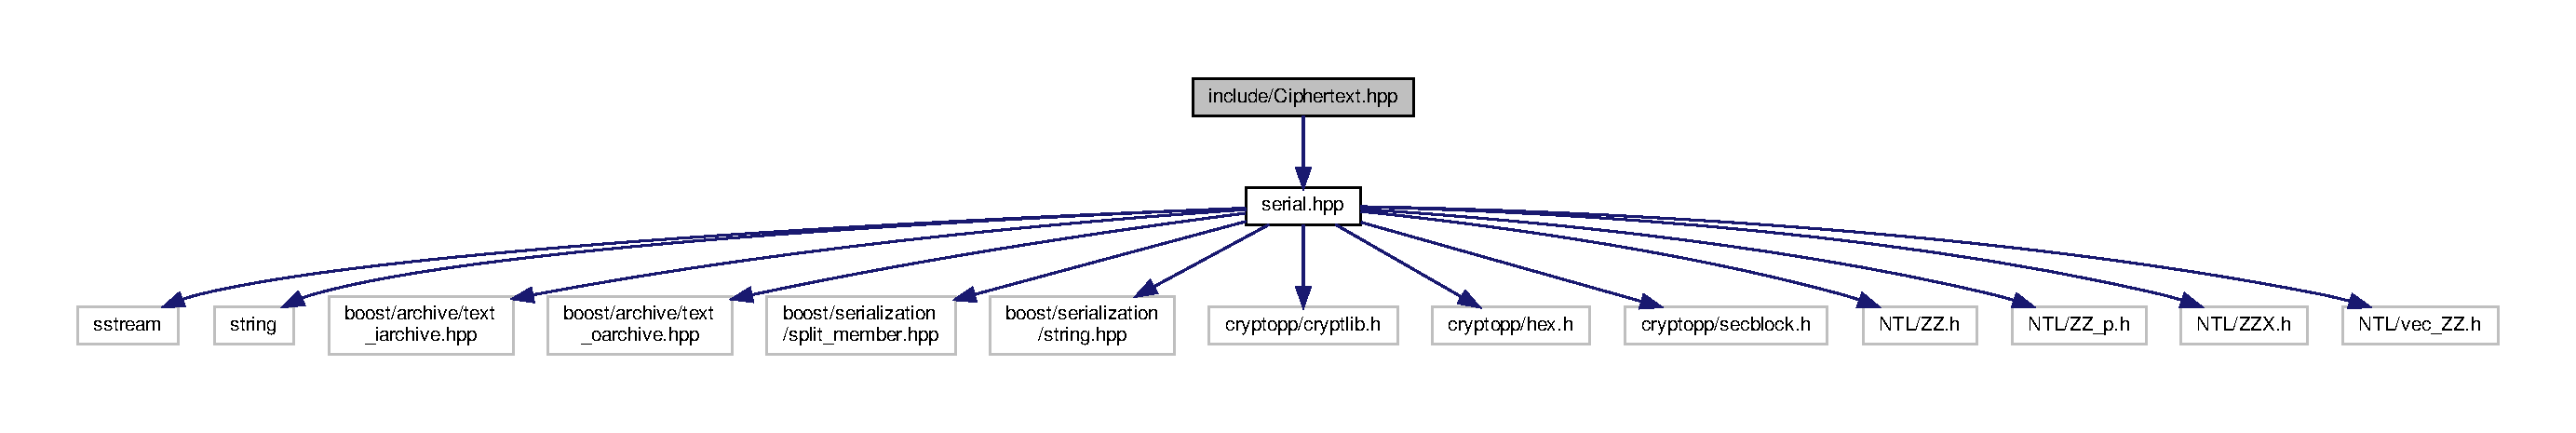
\includegraphics[width=350pt]{Ciphertext_8hpp__incl}
\end{center}
\end{figure}
This graph shows which files directly or indirectly include this file\+:
\nopagebreak
\begin{figure}[H]
\begin{center}
\leavevmode
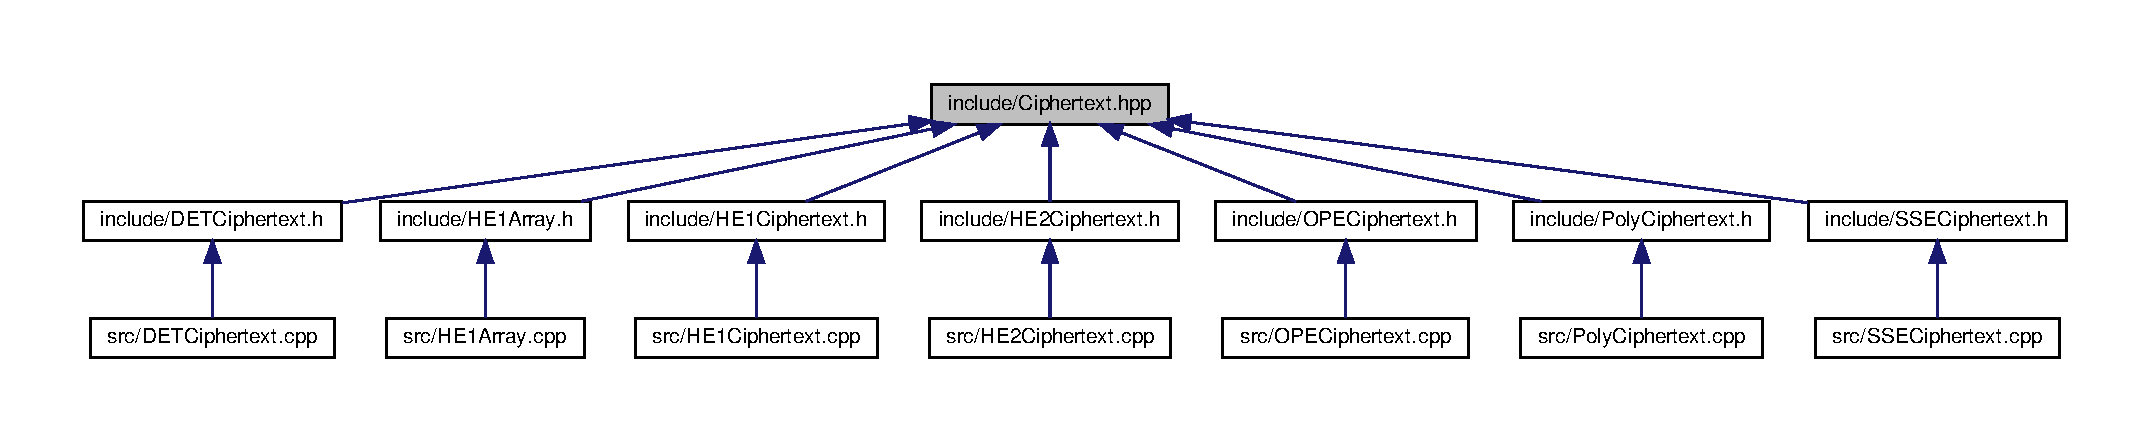
\includegraphics[width=350pt]{Ciphertext_8hpp__dep__incl}
\end{center}
\end{figure}
\subsection*{Classes}
\begin{DoxyCompactItemize}
\item 
class \hyperlink{classCiphertext}{Ciphertext$<$ T $>$}
\end{DoxyCompactItemize}

\hypertarget{DETCiphertext_8h}{}\section{include/\+D\+E\+T\+Ciphertext.h File Reference}
\label{DETCiphertext_8h}\index{include/\+D\+E\+T\+Ciphertext.\+h@{include/\+D\+E\+T\+Ciphertext.\+h}}
{\ttfamily \#include \char`\"{}Ciphertext.\+hpp\char`\"{}}\newline
Include dependency graph for D\+E\+T\+Ciphertext.\+h\+:
\nopagebreak
\begin{figure}[H]
\begin{center}
\leavevmode
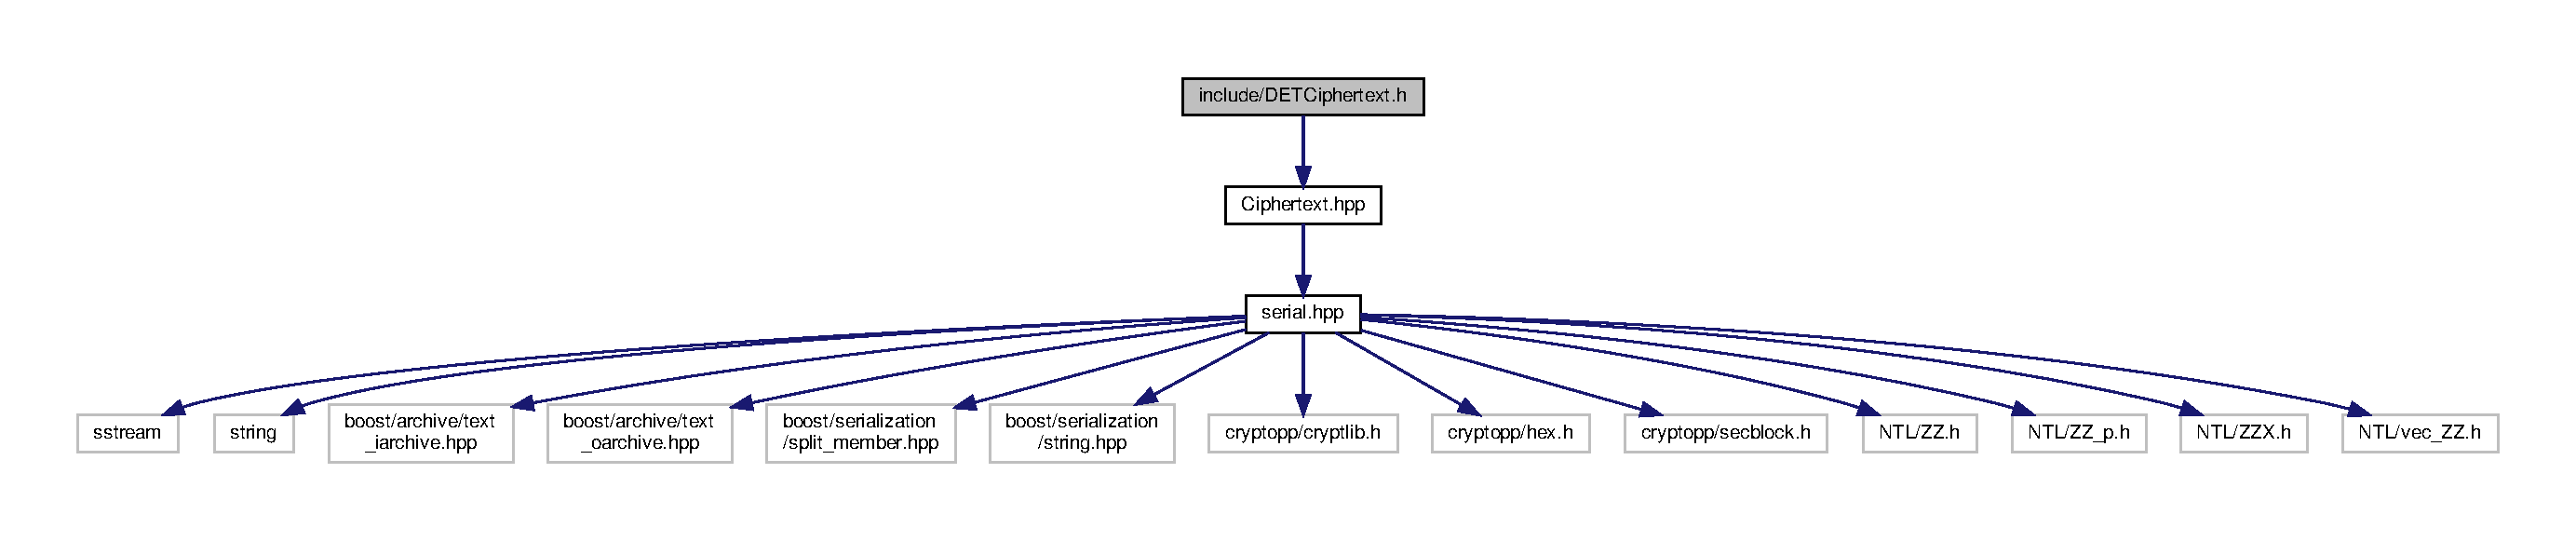
\includegraphics[width=350pt]{DETCiphertext_8h__incl}
\end{center}
\end{figure}
This graph shows which files directly or indirectly include this file\+:
\nopagebreak
\begin{figure}[H]
\begin{center}
\leavevmode
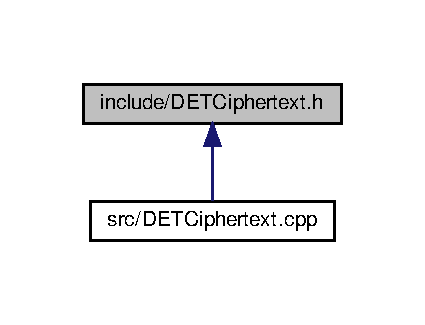
\includegraphics[width=204pt]{DETCiphertext_8h__dep__incl}
\end{center}
\end{figure}
\subsection*{Classes}
\begin{DoxyCompactItemize}
\item 
class \hyperlink{classDETCiphertext}{D\+E\+T\+Ciphertext}
\end{DoxyCompactItemize}

\hypertarget{HE1Array_8h}{}\section{include/\+H\+E1\+Array.h File Reference}
\label{HE1Array_8h}\index{include/\+H\+E1\+Array.\+h@{include/\+H\+E1\+Array.\+h}}
{\ttfamily \#include $<$vector$>$}\newline
{\ttfamily \#include $<$xmp.\+h$>$}\newline
{\ttfamily \#include $<$N\+T\+L/\+Z\+Z.\+h$>$}\newline
{\ttfamily \#include $<$N\+T\+L/vec\+\_\+\+Z\+Z.\+h$>$}\newline
{\ttfamily \#include \char`\"{}Ciphertext.\+hpp\char`\"{}}\newline
Include dependency graph for H\+E1\+Array.\+h\+:
\nopagebreak
\begin{figure}[H]
\begin{center}
\leavevmode
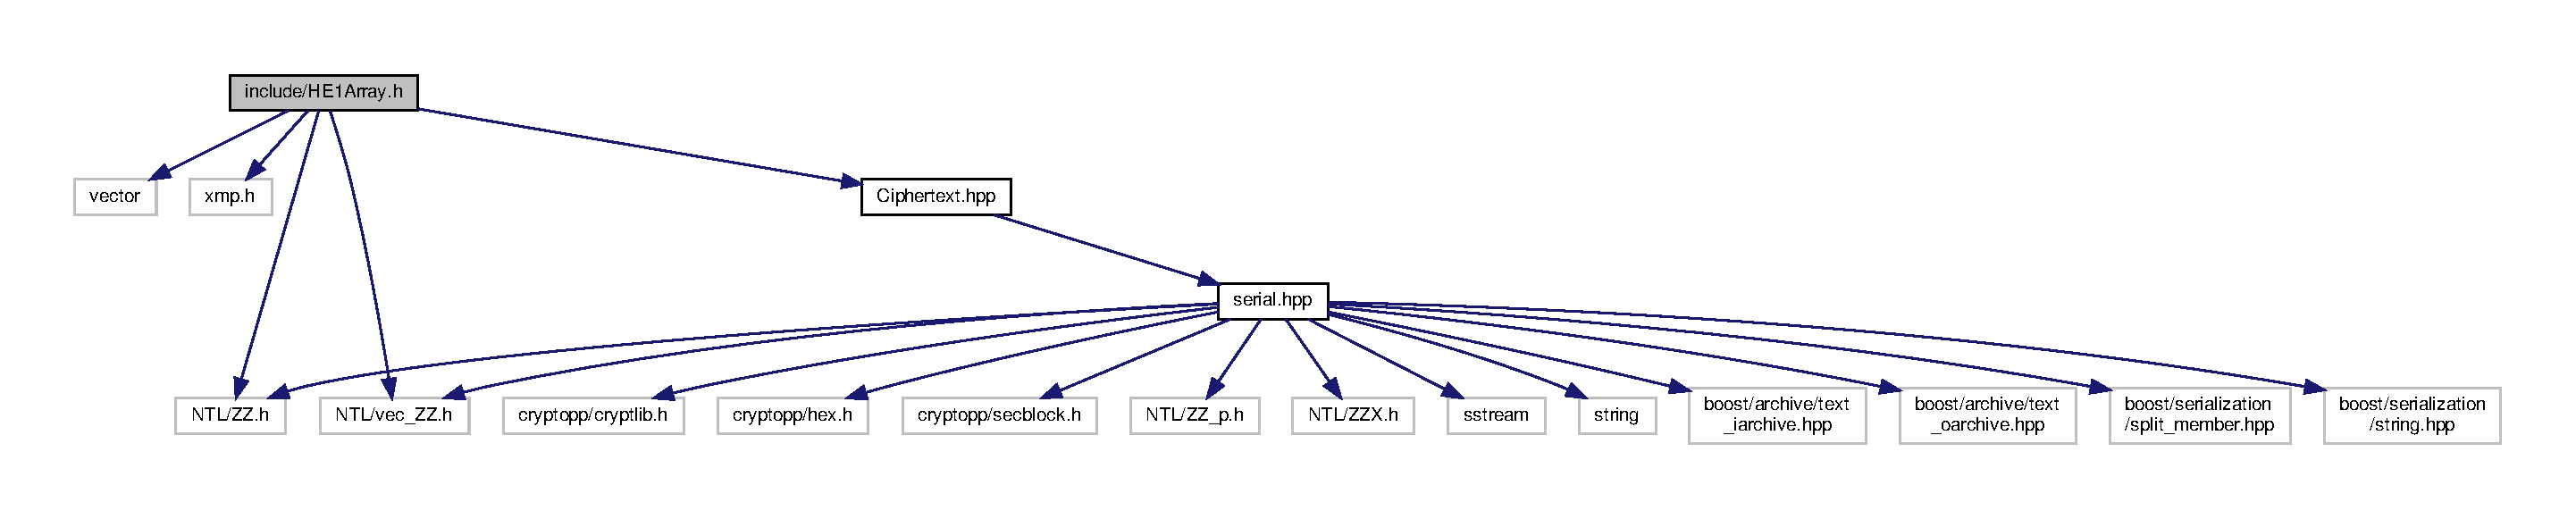
\includegraphics[width=350pt]{HE1Array_8h__incl}
\end{center}
\end{figure}
This graph shows which files directly or indirectly include this file\+:
\nopagebreak
\begin{figure}[H]
\begin{center}
\leavevmode
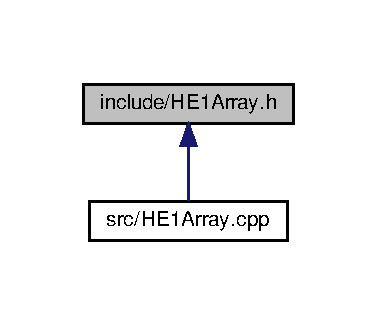
\includegraphics[width=181pt]{HE1Array_8h__dep__incl}
\end{center}
\end{figure}
\subsection*{Classes}
\begin{DoxyCompactItemize}
\item 
class \hyperlink{classHE1Array}{H\+E1\+Array}
\end{DoxyCompactItemize}
\subsection*{Macros}
\begin{DoxyCompactItemize}
\item 
\#define \hyperlink{HE1Array_8h_a1cedb291ba102a0ee52c1c23af18ace2}{X\+M\+P\+\_\+\+C\+H\+E\+C\+K\+\_\+\+E\+R\+R\+OR}(fun)
\end{DoxyCompactItemize}
\subsection*{Typedefs}
\begin{DoxyCompactItemize}
\item 
typedef uint8\+\_\+t \hyperlink{HE1Array_8h_ab8ef12fab634c171394422d0ee8baf94}{byte}
\item 
typedef uint32\+\_\+t \hyperlink{HE1Array_8h_a19036394f9c80a08fc846c96f668711c}{word}
\end{DoxyCompactItemize}


\subsection{Macro Definition Documentation}
\mbox{\Hypertarget{HE1Array_8h_a1cedb291ba102a0ee52c1c23af18ace2}\label{HE1Array_8h_a1cedb291ba102a0ee52c1c23af18ace2}} 
\index{H\+E1\+Array.\+h@{H\+E1\+Array.\+h}!X\+M\+P\+\_\+\+C\+H\+E\+C\+K\+\_\+\+E\+R\+R\+OR@{X\+M\+P\+\_\+\+C\+H\+E\+C\+K\+\_\+\+E\+R\+R\+OR}}
\index{X\+M\+P\+\_\+\+C\+H\+E\+C\+K\+\_\+\+E\+R\+R\+OR@{X\+M\+P\+\_\+\+C\+H\+E\+C\+K\+\_\+\+E\+R\+R\+OR}!H\+E1\+Array.\+h@{H\+E1\+Array.\+h}}
\subsubsection{\texorpdfstring{X\+M\+P\+\_\+\+C\+H\+E\+C\+K\+\_\+\+E\+R\+R\+OR}{XMP\_CHECK\_ERROR}}
{\footnotesize\ttfamily \#define X\+M\+P\+\_\+\+C\+H\+E\+C\+K\+\_\+\+E\+R\+R\+OR(\begin{DoxyParamCaption}\item[{}]{fun }\end{DoxyParamCaption})}

{\bfseries Value\+:}
\begin{DoxyCode}
\{                             \(\backslash\)
  xmpError\_t error=fun;     \(\backslash\)
  if(error!=xmpErrorSuccess)\{ \(\backslash\)
    if(error==xmpErrorCuda)   \(\backslash\)
      printf(\textcolor{stringliteral}{"CUDA Error %s, %s:%d\(\backslash\)n"},cudaGetErrorString(cudaGetLastError()),\_\_FILE\_\_,\_\_LINE\_\_); \(\backslash\)
    else  \(\backslash\)
      printf(\textcolor{stringliteral}{"XMP Error %s, %s:%d\(\backslash\)n"},xmpGetErrorString(error),\_\_FILE\_\_,\_\_LINE\_\_); \(\backslash\)
    exit(EXIT\_FAILURE); \(\backslash\)
  \} \(\backslash\)
\}
\end{DoxyCode}
Macro to convert the X\+MP error code to a user-\/friendly string and then exit the program with a failure code 

\subsection{Typedef Documentation}
\mbox{\Hypertarget{HE1Array_8h_ab8ef12fab634c171394422d0ee8baf94}\label{HE1Array_8h_ab8ef12fab634c171394422d0ee8baf94}} 
\index{H\+E1\+Array.\+h@{H\+E1\+Array.\+h}!byte@{byte}}
\index{byte@{byte}!H\+E1\+Array.\+h@{H\+E1\+Array.\+h}}
\subsubsection{\texorpdfstring{byte}{byte}}
{\footnotesize\ttfamily typedef uint8\+\_\+t \hyperlink{HE1Array_8h_ab8ef12fab634c171394422d0ee8baf94}{byte}}

Defines a {\ttfamily byte} as an unsigned 8 bit integer \mbox{\Hypertarget{HE1Array_8h_a19036394f9c80a08fc846c96f668711c}\label{HE1Array_8h_a19036394f9c80a08fc846c96f668711c}} 
\index{H\+E1\+Array.\+h@{H\+E1\+Array.\+h}!word@{word}}
\index{word@{word}!H\+E1\+Array.\+h@{H\+E1\+Array.\+h}}
\subsubsection{\texorpdfstring{word}{word}}
{\footnotesize\ttfamily typedef uint32\+\_\+t \hyperlink{HE1Array_8h_a19036394f9c80a08fc846c96f668711c}{word}}

Defines a {\ttfamily word} as an unsigned 32 bit integer 
\hypertarget{HE1Ciphertext_8h}{}\section{include/\+H\+E1\+Ciphertext.h File Reference}
\label{HE1Ciphertext_8h}\index{include/\+H\+E1\+Ciphertext.\+h@{include/\+H\+E1\+Ciphertext.\+h}}
{\ttfamily \#include $<$string$>$}\newline
{\ttfamily \#include $<$sstream$>$}\newline
{\ttfamily \#include $<$N\+T\+L/\+Z\+Z.\+h$>$}\newline
{\ttfamily \#include $<$N\+T\+L/\+Z\+Z\+\_\+p.\+h$>$}\newline
{\ttfamily \#include $<$boost/archive/text\+\_\+iarchive.\+hpp$>$}\newline
{\ttfamily \#include $<$boost/archive/text\+\_\+oarchive.\+hpp$>$}\newline
{\ttfamily \#include $<$boost/serialization/split\+\_\+member.\+hpp$>$}\newline
{\ttfamily \#include $<$boost/serialization/string.\+hpp$>$}\newline
{\ttfamily \#include \char`\"{}Ciphertext.\+hpp\char`\"{}}\newline
Include dependency graph for H\+E1\+Ciphertext.\+h\+:
\nopagebreak
\begin{figure}[H]
\begin{center}
\leavevmode
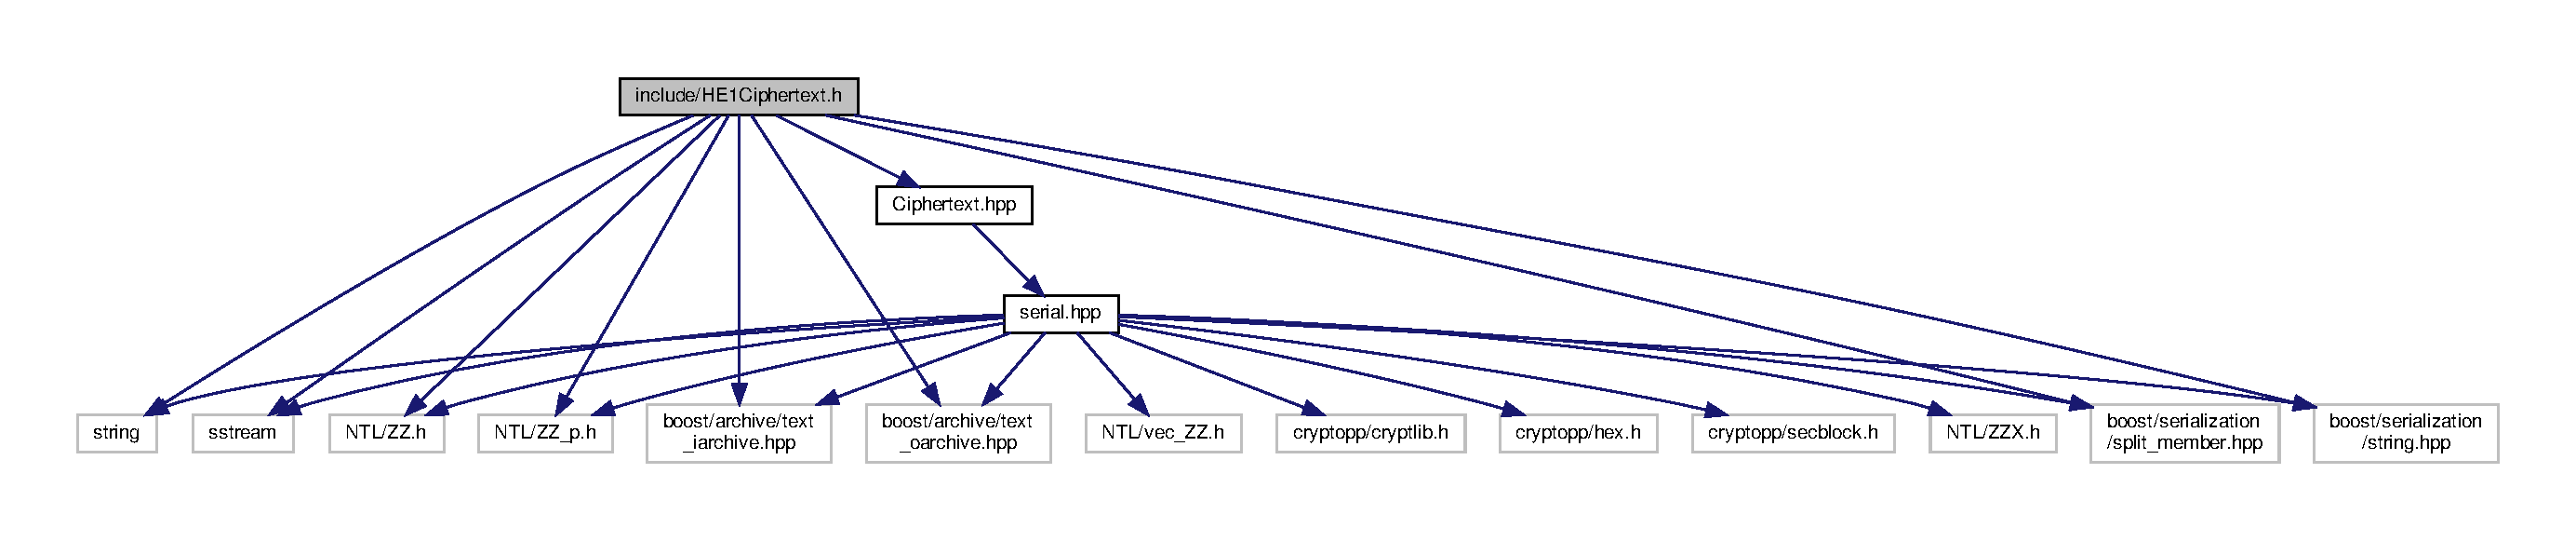
\includegraphics[width=350pt]{HE1Ciphertext_8h__incl}
\end{center}
\end{figure}
This graph shows which files directly or indirectly include this file\+:
\nopagebreak
\begin{figure}[H]
\begin{center}
\leavevmode
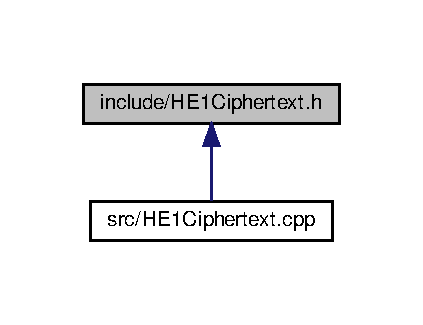
\includegraphics[width=203pt]{HE1Ciphertext_8h__dep__incl}
\end{center}
\end{figure}
\subsection*{Classes}
\begin{DoxyCompactItemize}
\item 
class \hyperlink{classHE1Ciphertext}{H\+E1\+Ciphertext}
\end{DoxyCompactItemize}

\hypertarget{HE2Ciphertext_8h}{}\section{include/\+H\+E2\+Ciphertext.h File Reference}
\label{HE2Ciphertext_8h}\index{include/\+H\+E2\+Ciphertext.\+h@{include/\+H\+E2\+Ciphertext.\+h}}
{\ttfamily \#include $<$N\+T\+L/\+Z\+Z.\+h$>$}\newline
{\ttfamily \#include $<$N\+T\+L/vec\+\_\+\+Z\+Z\+\_\+p.\+h$>$}\newline
{\ttfamily \#include $<$N\+T\+L/mat\+\_\+\+Z\+Z\+\_\+p.\+h$>$}\newline
{\ttfamily \#include \char`\"{}Ciphertext.\+hpp\char`\"{}}\newline
Include dependency graph for H\+E2\+Ciphertext.\+h\+:
\nopagebreak
\begin{figure}[H]
\begin{center}
\leavevmode
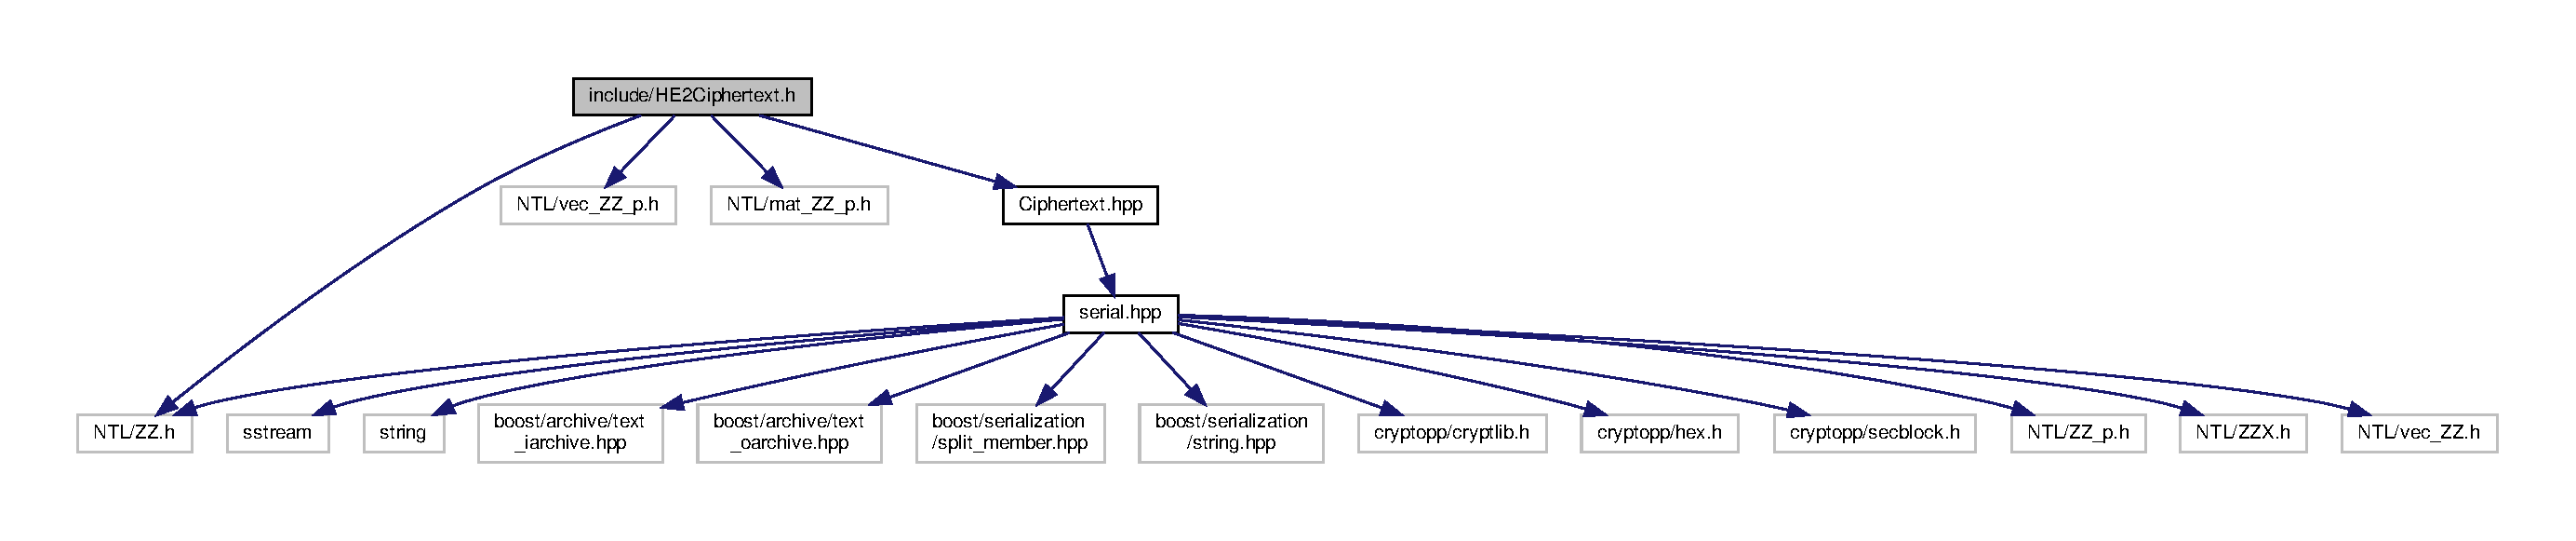
\includegraphics[width=350pt]{HE2Ciphertext_8h__incl}
\end{center}
\end{figure}
This graph shows which files directly or indirectly include this file\+:
\nopagebreak
\begin{figure}[H]
\begin{center}
\leavevmode
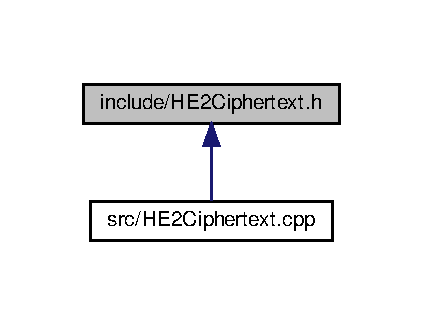
\includegraphics[width=203pt]{HE2Ciphertext_8h__dep__incl}
\end{center}
\end{figure}
\subsection*{Classes}
\begin{DoxyCompactItemize}
\item 
class \hyperlink{classHE2Ciphertext}{H\+E2\+Ciphertext}
\end{DoxyCompactItemize}

\hypertarget{OPECiphertext_8h}{}\section{include/\+O\+P\+E\+Ciphertext.h File Reference}
\label{OPECiphertext_8h}\index{include/\+O\+P\+E\+Ciphertext.\+h@{include/\+O\+P\+E\+Ciphertext.\+h}}
{\ttfamily \#include \char`\"{}Ciphertext.\+hpp\char`\"{}}\newline
Include dependency graph for O\+P\+E\+Ciphertext.\+h\+:
\nopagebreak
\begin{figure}[H]
\begin{center}
\leavevmode
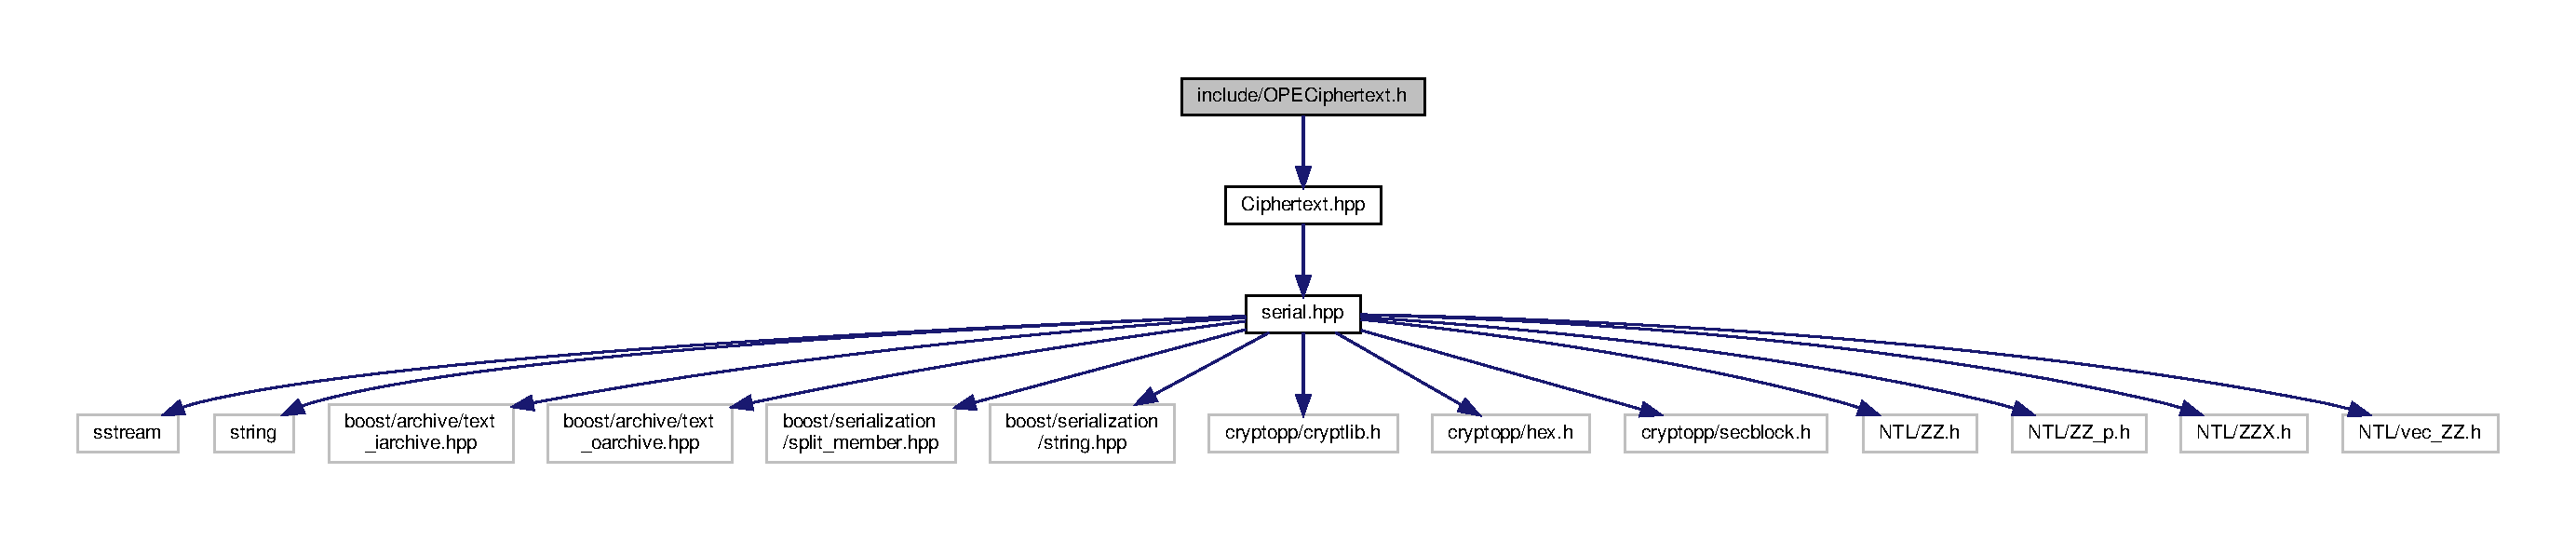
\includegraphics[width=350pt]{OPECiphertext_8h__incl}
\end{center}
\end{figure}
This graph shows which files directly or indirectly include this file\+:
\nopagebreak
\begin{figure}[H]
\begin{center}
\leavevmode
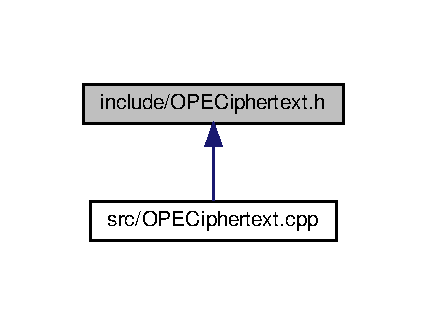
\includegraphics[width=205pt]{OPECiphertext_8h__dep__incl}
\end{center}
\end{figure}
\subsection*{Classes}
\begin{DoxyCompactItemize}
\item 
class \hyperlink{classOPECiphertext}{O\+P\+E\+Ciphertext}
\end{DoxyCompactItemize}

\hypertarget{PolyCiphertext_8h}{}\section{include/\+Poly\+Ciphertext.h File Reference}
\label{PolyCiphertext_8h}\index{include/\+Poly\+Ciphertext.\+h@{include/\+Poly\+Ciphertext.\+h}}
{\ttfamily \#include $<$vector$>$}\newline
{\ttfamily \#include $<$string$>$}\newline
{\ttfamily \#include $<$N\+T\+L/\+Z\+Z\+X.\+h$>$}\newline
{\ttfamily \#include $<$N\+T\+L/vec\+\_\+\+Z\+Z.\+h$>$}\newline
{\ttfamily \#include $<$boost/archive/text\+\_\+iarchive.\+hpp$>$}\newline
{\ttfamily \#include $<$boost/archive/text\+\_\+oarchive.\+hpp$>$}\newline
{\ttfamily \#include \char`\"{}Ciphertext.\+hpp\char`\"{}}\newline
Include dependency graph for Poly\+Ciphertext.\+h\+:
\nopagebreak
\begin{figure}[H]
\begin{center}
\leavevmode
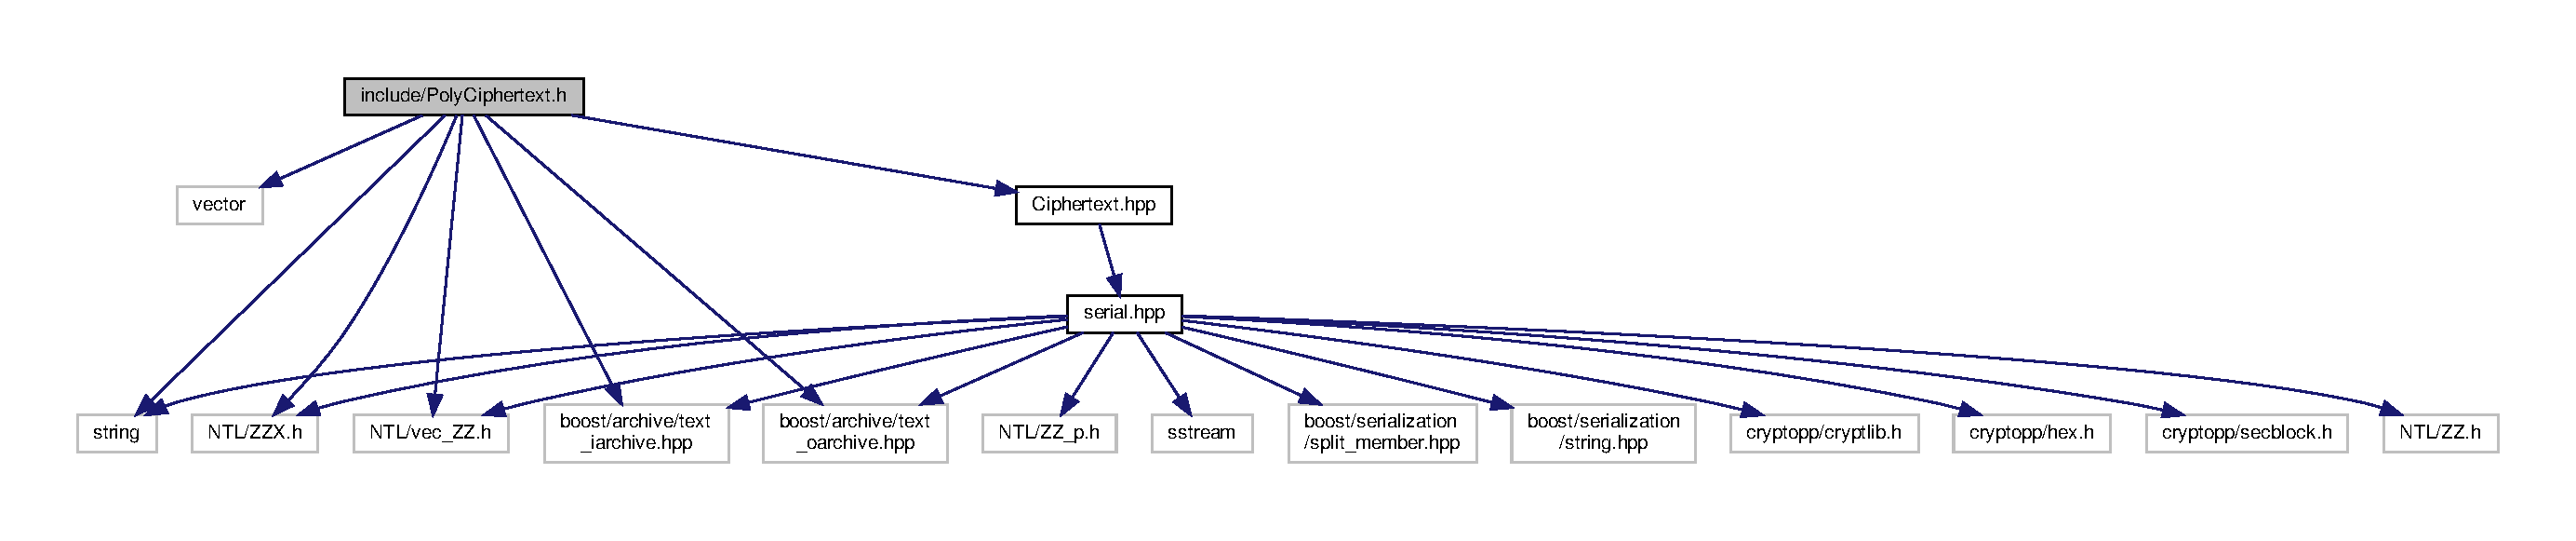
\includegraphics[width=350pt]{PolyCiphertext_8h__incl}
\end{center}
\end{figure}
This graph shows which files directly or indirectly include this file\+:
\nopagebreak
\begin{figure}[H]
\begin{center}
\leavevmode
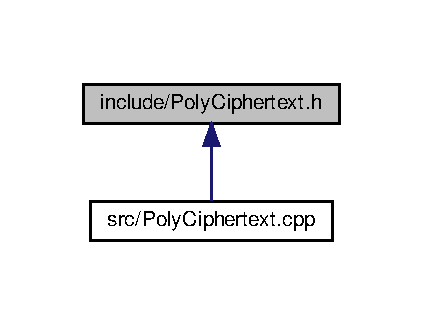
\includegraphics[width=203pt]{PolyCiphertext_8h__dep__incl}
\end{center}
\end{figure}
\subsection*{Classes}
\begin{DoxyCompactItemize}
\item 
class \hyperlink{classPolyCiphertext}{Poly\+Ciphertext}
\end{DoxyCompactItemize}

\hypertarget{serial_8hpp}{}\section{include/serial.hpp File Reference}
\label{serial_8hpp}\index{include/serial.\+hpp@{include/serial.\+hpp}}
{\ttfamily \#include $<$sstream$>$}\newline
{\ttfamily \#include $<$string$>$}\newline
{\ttfamily \#include $<$boost/archive/text\+\_\+iarchive.\+hpp$>$}\newline
{\ttfamily \#include $<$boost/archive/text\+\_\+oarchive.\+hpp$>$}\newline
{\ttfamily \#include $<$boost/serialization/split\+\_\+member.\+hpp$>$}\newline
{\ttfamily \#include $<$boost/serialization/string.\+hpp$>$}\newline
{\ttfamily \#include $<$cryptopp/cryptlib.\+h$>$}\newline
{\ttfamily \#include $<$cryptopp/hex.\+h$>$}\newline
{\ttfamily \#include $<$cryptopp/secblock.\+h$>$}\newline
{\ttfamily \#include $<$N\+T\+L/\+Z\+Z.\+h$>$}\newline
{\ttfamily \#include $<$N\+T\+L/\+Z\+Z\+\_\+p.\+h$>$}\newline
{\ttfamily \#include $<$N\+T\+L/\+Z\+Z\+X.\+h$>$}\newline
{\ttfamily \#include $<$N\+T\+L/vec\+\_\+\+Z\+Z.\+h$>$}\newline
Include dependency graph for serial.\+hpp\+:
\nopagebreak
\begin{figure}[H]
\begin{center}
\leavevmode
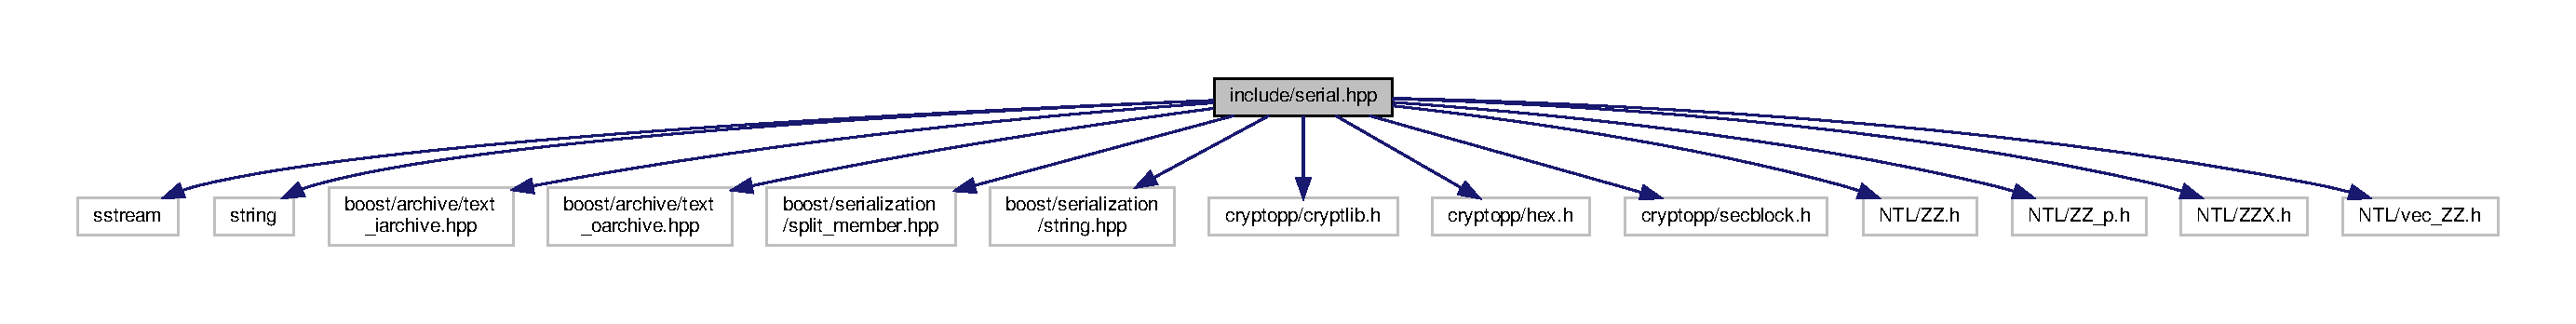
\includegraphics[width=350pt]{serial_8hpp__incl}
\end{center}
\end{figure}
This graph shows which files directly or indirectly include this file\+:
\nopagebreak
\begin{figure}[H]
\begin{center}
\leavevmode
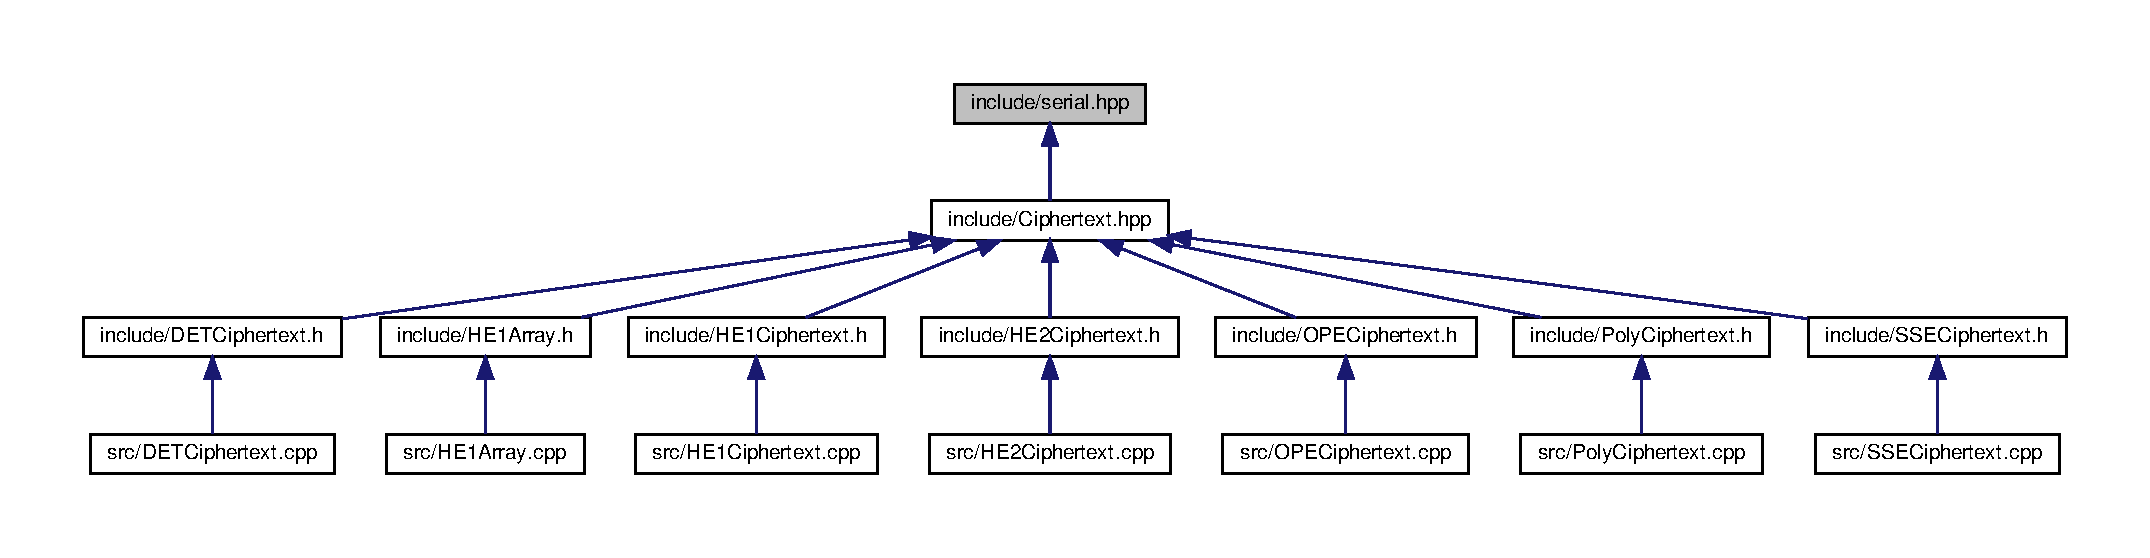
\includegraphics[width=350pt]{serial_8hpp__dep__incl}
\end{center}
\end{figure}
\subsection*{Namespaces}
\begin{DoxyCompactItemize}
\item 
 \hyperlink{namespaceboost}{boost}
\item 
 \hyperlink{namespaceboost_1_1serialization}{boost\+::serialization}
\end{DoxyCompactItemize}
\subsection*{Functions}
\begin{DoxyCompactItemize}
\item 
{\footnotesize template$<$class Archive $>$ }\\void \hyperlink{namespaceboost_1_1serialization_a7c8cd6b4a705476128a04299a9d0ab02}{boost\+::serialization\+::save} (Archive \&ar, const N\+T\+L\+::\+ZZ \&p, const unsigned int version)
\item 
{\footnotesize template$<$class Archive $>$ }\\void \hyperlink{namespaceboost_1_1serialization_ac9d9d4bc06458befc413756326393db1}{boost\+::serialization\+::load} (Archive \&ar, N\+T\+L\+::\+ZZ \&p, const unsigned int version)
\item 
{\footnotesize template$<$class Archive $>$ }\\void \hyperlink{namespaceboost_1_1serialization_ac305bc4c0e58113a47100a24ff100480}{boost\+::serialization\+::serialize} (Archive \&ar, N\+T\+L\+::\+ZZ \&p, const unsigned int version)
\item 
{\footnotesize template$<$class Archive $>$ }\\void \hyperlink{namespaceboost_1_1serialization_a9d93508b5efacb662d1ab755d3d9b828}{boost\+::serialization\+::save} (Archive \&ar, const N\+T\+L\+::\+Z\+Z\+\_\+p \&p, const unsigned int version)
\item 
{\footnotesize template$<$class Archive $>$ }\\void \hyperlink{namespaceboost_1_1serialization_a010ed145b746e6d7c5d4e643ff39145b}{boost\+::serialization\+::load} (Archive \&ar, N\+T\+L\+::\+Z\+Z\+\_\+p \&p, const unsigned int version)
\item 
{\footnotesize template$<$class Archive $>$ }\\void \hyperlink{namespaceboost_1_1serialization_a8f14c5980a9e7f5b1f04f96cb7ef6054}{boost\+::serialization\+::serialize} (Archive \&ar, N\+T\+L\+::\+Z\+Z\+\_\+p \&p, const unsigned int version)
\item 
{\footnotesize template$<$class Archive $>$ }\\void \hyperlink{namespaceboost_1_1serialization_a02839a8348cf5e4adfac1f031eb0bf02}{boost\+::serialization\+::save} (Archive \&ar, const N\+T\+L\+::\+Z\+ZX \&p, const unsigned int version)
\item 
{\footnotesize template$<$class Archive $>$ }\\void \hyperlink{namespaceboost_1_1serialization_a7b78d5cf4b5caa328bef6a087fbaff9c}{boost\+::serialization\+::load} (Archive \&ar, N\+T\+L\+::\+Z\+ZX \&p, const unsigned int version)
\item 
{\footnotesize template$<$class Archive $>$ }\\void \hyperlink{namespaceboost_1_1serialization_a0734cf2ae9e8ce324e5d26bdea7afd70}{boost\+::serialization\+::serialize} (Archive \&ar, N\+T\+L\+::\+Z\+ZX \&p, const unsigned int version)
\item 
{\footnotesize template$<$class Archive $>$ }\\void \hyperlink{namespaceboost_1_1serialization_a58966b07928230bb0400b6117217baa1}{boost\+::serialization\+::save} (Archive \&ar, const N\+T\+L\+::vec\+\_\+\+ZZ \&p, const unsigned int version)
\item 
{\footnotesize template$<$class Archive $>$ }\\void \hyperlink{namespaceboost_1_1serialization_a020abf1a3721352f3f93367e476adb75}{boost\+::serialization\+::load} (Archive \&ar, N\+T\+L\+::vec\+\_\+\+ZZ \&p, const unsigned int version)
\item 
{\footnotesize template$<$class Archive $>$ }\\void \hyperlink{namespaceboost_1_1serialization_aeb170b7c609eb6350c2bcf3331d6f140}{boost\+::serialization\+::serialize} (Archive \&ar, N\+T\+L\+::vec\+\_\+\+ZZ \&p, const unsigned int version)
\item 
{\footnotesize template$<$class Archive $>$ }\\void \hyperlink{namespaceboost_1_1serialization_acd0cd0062652d786e7d0d108a7844d1c}{boost\+::serialization\+::save} (Archive \&ar, const N\+T\+L\+::vec\+\_\+\+Z\+Z\+\_\+p \&p, const unsigned int version)
\item 
{\footnotesize template$<$class Archive $>$ }\\void \hyperlink{namespaceboost_1_1serialization_afd8ccb691b59647d2c043b64fe0ea28d}{boost\+::serialization\+::load} (Archive \&ar, N\+T\+L\+::vec\+\_\+\+Z\+Z\+\_\+p \&p, const unsigned int version)
\item 
{\footnotesize template$<$class Archive $>$ }\\void \hyperlink{namespaceboost_1_1serialization_a7b255d9449f6f4f7b5e3ca7c054cb2c3}{boost\+::serialization\+::serialize} (Archive \&ar, N\+T\+L\+::vec\+\_\+\+Z\+Z\+\_\+p \&p, const unsigned int version)
\item 
{\footnotesize template$<$class Archive $>$ }\\void \hyperlink{namespaceboost_1_1serialization_a435bf2f49b7036c361876e915fed6b53}{boost\+::serialization\+::save} (Archive \&ar, const Crypto\+P\+P\+::\+Sec\+Byte\+Block \&p, const unsigned int version)
\item 
{\footnotesize template$<$class Archive $>$ }\\void \hyperlink{namespaceboost_1_1serialization_ac8d644880f4596e04671aa5db78527ff}{boost\+::serialization\+::load} (Archive \&ar, Crypto\+P\+P\+::\+Sec\+Byte\+Block \&p, const unsigned int version)
\item 
{\footnotesize template$<$class Archive $>$ }\\void \hyperlink{namespaceboost_1_1serialization_a62de9ba81b8b564ae450120250a7d597}{boost\+::serialization\+::serialize} (Archive \&ar, Crypto\+P\+P\+::\+Sec\+Byte\+Block \&p, const unsigned int version)
\end{DoxyCompactItemize}

\hypertarget{SSECiphertext_8h}{}\section{include/\+S\+S\+E\+Ciphertext.h File Reference}
\label{SSECiphertext_8h}\index{include/\+S\+S\+E\+Ciphertext.\+h@{include/\+S\+S\+E\+Ciphertext.\+h}}
{\ttfamily \#include $<$cryptopp/cryptlib.\+h$>$}\newline
{\ttfamily \#include $<$cryptopp/aes.\+h$>$}\newline
{\ttfamily \#include $<$cryptopp/cmac.\+h$>$}\newline
{\ttfamily \#include $<$cryptopp/secblock.\+h$>$}\newline
{\ttfamily \#include \char`\"{}Ciphertext.\+hpp\char`\"{}}\newline
Include dependency graph for S\+S\+E\+Ciphertext.\+h\+:
\nopagebreak
\begin{figure}[H]
\begin{center}
\leavevmode
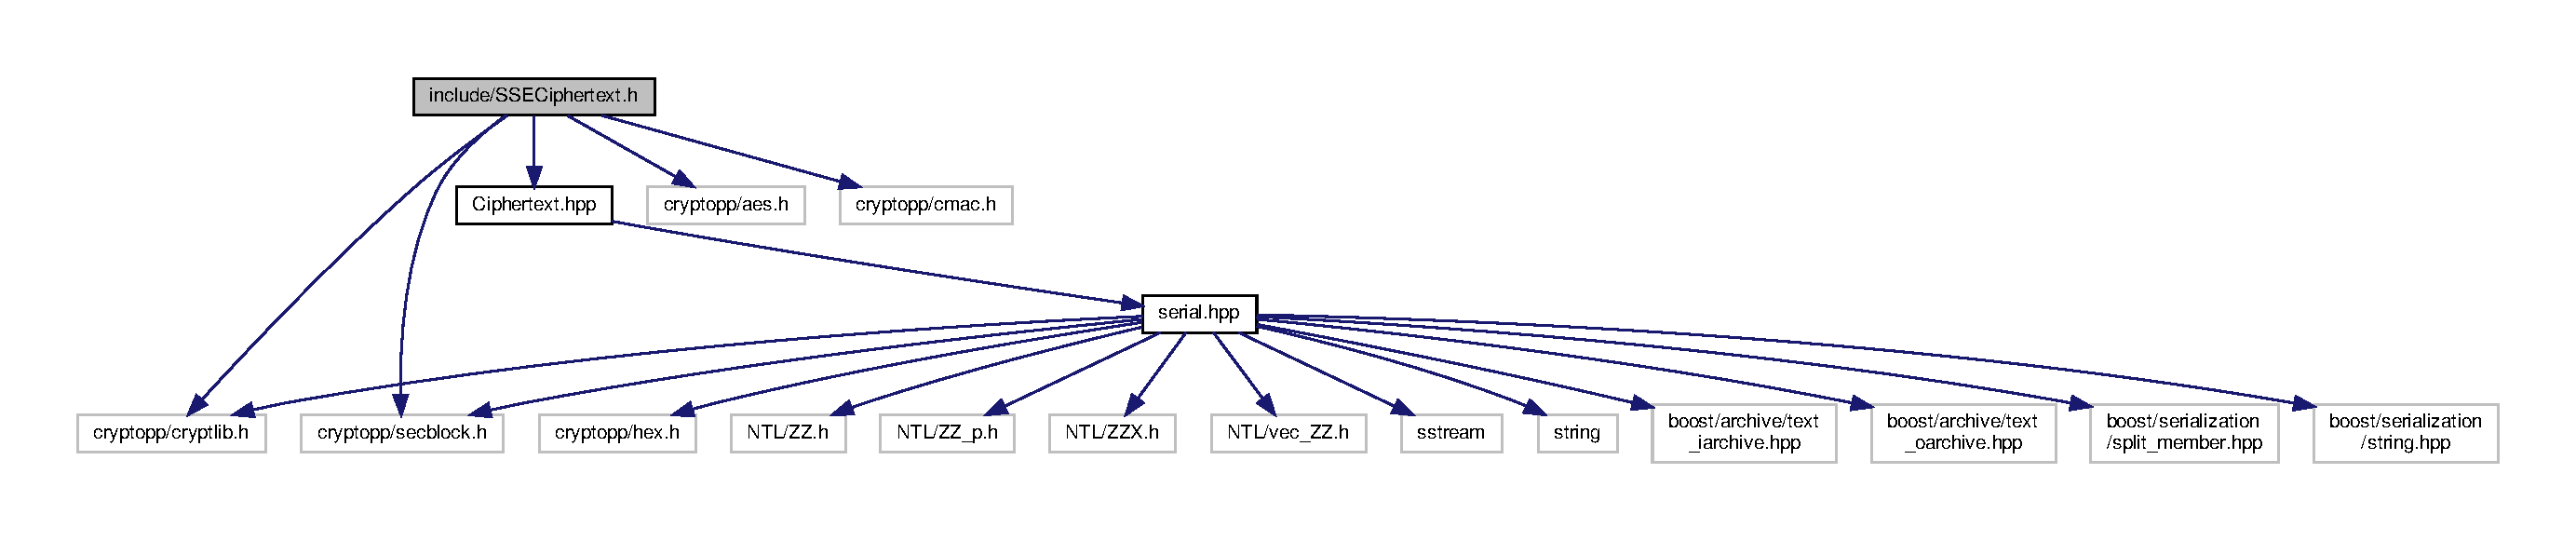
\includegraphics[width=350pt]{SSECiphertext_8h__incl}
\end{center}
\end{figure}
This graph shows which files directly or indirectly include this file\+:
\nopagebreak
\begin{figure}[H]
\begin{center}
\leavevmode
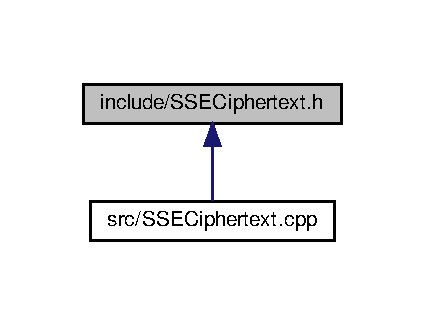
\includegraphics[width=204pt]{SSECiphertext_8h__dep__incl}
\end{center}
\end{figure}
\subsection*{Classes}
\begin{DoxyCompactItemize}
\item 
class \hyperlink{classSSECiphertext}{S\+S\+E\+Ciphertext}
\end{DoxyCompactItemize}

\hypertarget{DETCiphertext_8cpp}{}\section{src/\+D\+E\+T\+Ciphertext.cpp File Reference}
\label{DETCiphertext_8cpp}\index{src/\+D\+E\+T\+Ciphertext.\+cpp@{src/\+D\+E\+T\+Ciphertext.\+cpp}}
{\ttfamily \#include \char`\"{}D\+E\+T\+Ciphertext.\+h\char`\"{}}\newline
Include dependency graph for D\+E\+T\+Ciphertext.\+cpp\+:
\nopagebreak
\begin{figure}[H]
\begin{center}
\leavevmode
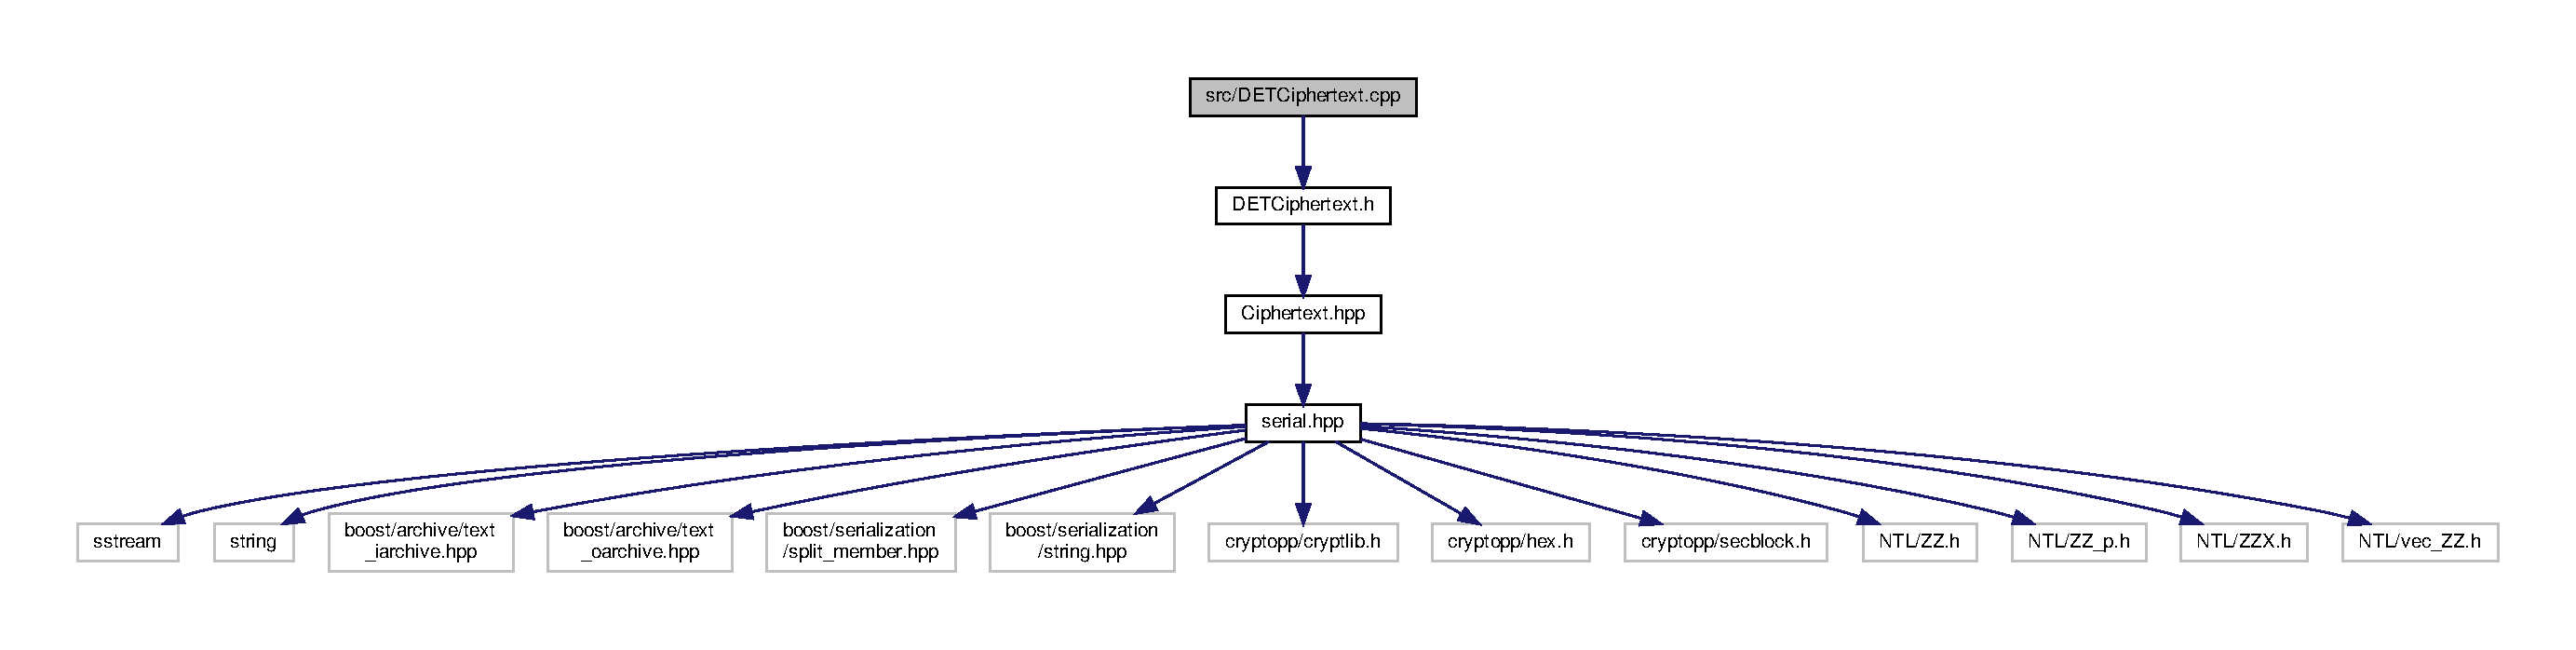
\includegraphics[width=350pt]{DETCiphertext_8cpp__incl}
\end{center}
\end{figure}
\subsection*{Functions}
\begin{DoxyCompactItemize}
\item 
bool \hyperlink{DETCiphertext_8cpp_a5f7e97804478b1b2badc92d540797b73}{operator==} (\hyperlink{classDETCiphertext}{D\+E\+T\+Ciphertext} \&a, \hyperlink{classDETCiphertext}{D\+E\+T\+Ciphertext} \&b)
\end{DoxyCompactItemize}


\subsection{Function Documentation}
\mbox{\Hypertarget{DETCiphertext_8cpp_a5f7e97804478b1b2badc92d540797b73}\label{DETCiphertext_8cpp_a5f7e97804478b1b2badc92d540797b73}} 
\index{D\+E\+T\+Ciphertext.\+cpp@{D\+E\+T\+Ciphertext.\+cpp}!operator==@{operator==}}
\index{operator==@{operator==}!D\+E\+T\+Ciphertext.\+cpp@{D\+E\+T\+Ciphertext.\+cpp}}
\subsubsection{\texorpdfstring{operator==()}{operator==()}}
{\footnotesize\ttfamily bool operator== (\begin{DoxyParamCaption}\item[{\hyperlink{classDETCiphertext}{D\+E\+T\+Ciphertext} \&}]{a,  }\item[{\hyperlink{classDETCiphertext}{D\+E\+T\+Ciphertext} \&}]{b }\end{DoxyParamCaption})}

Return {\ttfamily a.\+ciphertext} = {\ttfamily b.\+ciphertext} 
\begin{DoxyParams}{Parameters}
{\em a} & A {\ttfamily \hyperlink{classDETCiphertext}{D\+E\+T\+Ciphertext}} object \\
\hline
{\em b} & A {\ttfamily \hyperlink{classDETCiphertext}{D\+E\+T\+Ciphertext}} object \\
\hline
\end{DoxyParams}
\begin{DoxyReturn}{Returns}
{\ttfamily true} or {\ttfamily false} 
\end{DoxyReturn}

\hypertarget{HE1Array_8cpp}{}\section{src/\+H\+E1\+Array.cpp File Reference}
\label{HE1Array_8cpp}\index{src/\+H\+E1\+Array.\+cpp@{src/\+H\+E1\+Array.\+cpp}}
{\ttfamily \#include \char`\"{}H\+E1\+Array.\+h\char`\"{}}\newline
Include dependency graph for H\+E1\+Array.\+cpp\+:
\nopagebreak
\begin{figure}[H]
\begin{center}
\leavevmode
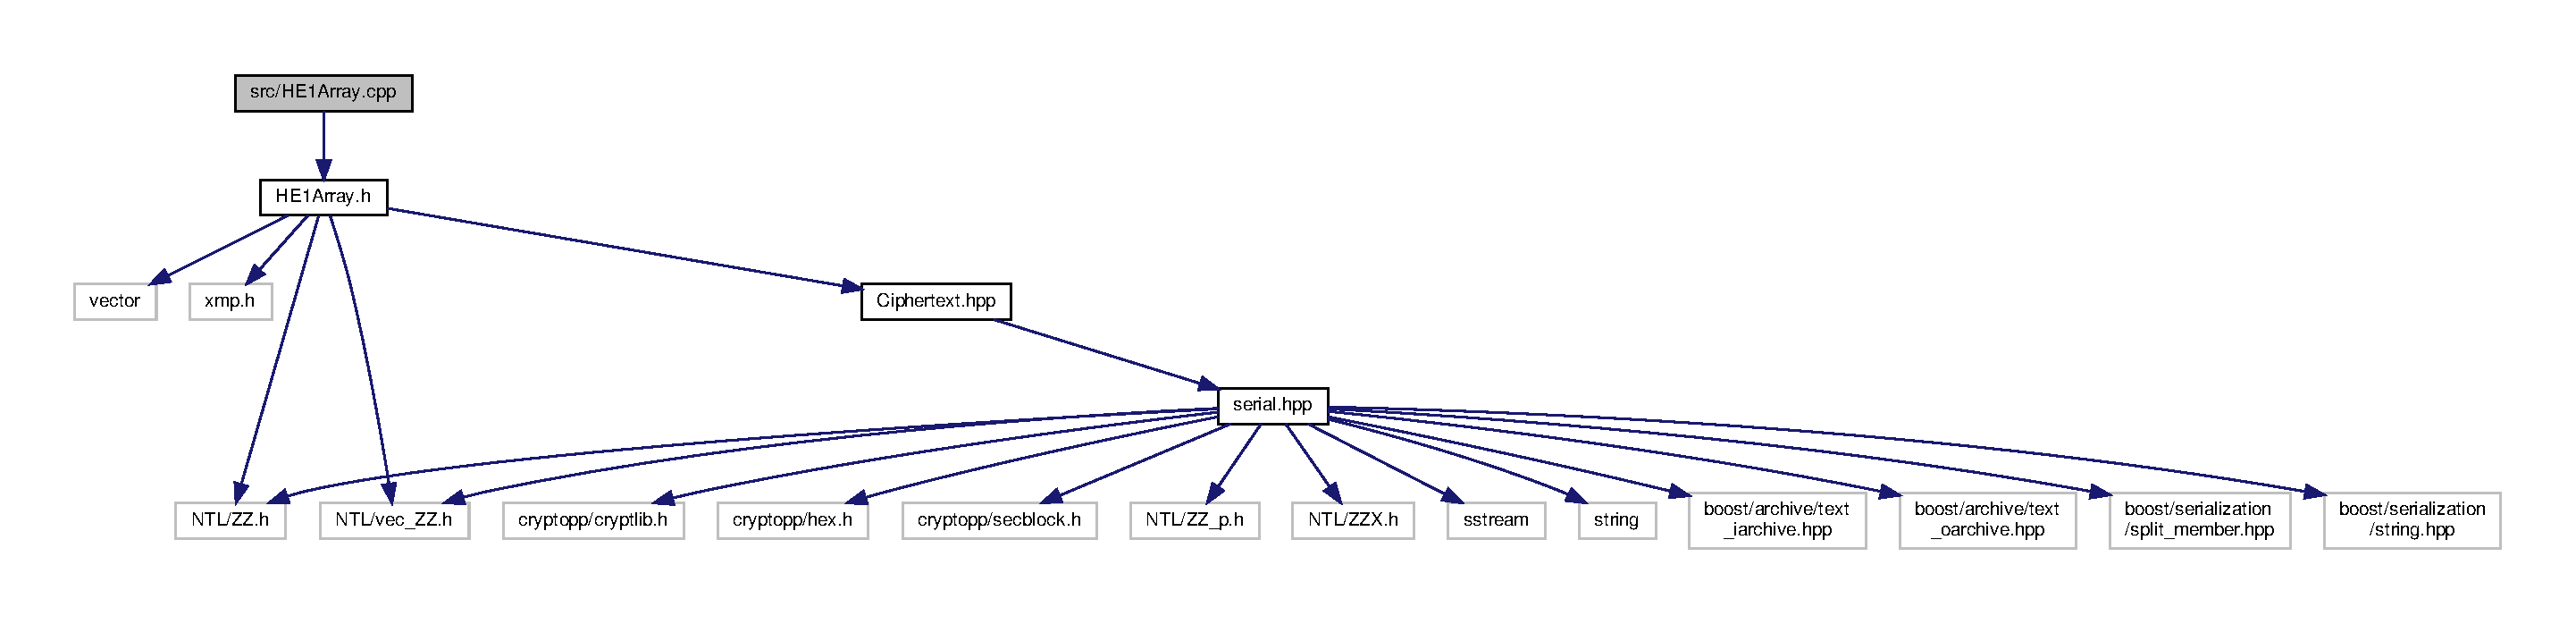
\includegraphics[width=350pt]{HE1Array_8cpp__incl}
\end{center}
\end{figure}
\subsection*{Functions}
\begin{DoxyCompactItemize}
\item 
\hyperlink{classHE1Array}{H\+E1\+Array} \hyperlink{HE1Array_8cpp_aaa51e336d1bca00b78a39445cc9525ec}{operator+} (\hyperlink{classHE1Array}{H\+E1\+Array} \&a, \hyperlink{classHE1Array}{H\+E1\+Array} \&b)
\item 
\hyperlink{classHE1Array}{H\+E1\+Array} \hyperlink{HE1Array_8cpp_a9af458afd1fae2464406a71868d411d9}{operator$\ast$} (\hyperlink{classHE1Array}{H\+E1\+Array} \&a, \hyperlink{classHE1Array}{H\+E1\+Array} \&b)
\end{DoxyCompactItemize}


\subsection{Function Documentation}
\mbox{\Hypertarget{HE1Array_8cpp_a9af458afd1fae2464406a71868d411d9}\label{HE1Array_8cpp_a9af458afd1fae2464406a71868d411d9}} 
\index{H\+E1\+Array.\+cpp@{H\+E1\+Array.\+cpp}!operator$\ast$@{operator$\ast$}}
\index{operator$\ast$@{operator$\ast$}!H\+E1\+Array.\+cpp@{H\+E1\+Array.\+cpp}}
\subsubsection{\texorpdfstring{operator$\ast$()}{operator*()}}
{\footnotesize\ttfamily \hyperlink{classHE1Array}{H\+E1\+Array} operator$\ast$ (\begin{DoxyParamCaption}\item[{\hyperlink{classHE1Array}{H\+E1\+Array} \&}]{a,  }\item[{\hyperlink{classHE1Array}{H\+E1\+Array} \&}]{b }\end{DoxyParamCaption})}

Performs modular multiplication the two {\ttfamily xmp\+Integers\+\_\+t} member arrays ({\ttfamily ciphertext} ) elementwise and returns a new object containing the array of sums 
\begin{DoxyParams}{Parameters}
{\em a} & A {\ttfamily \hyperlink{classHE1Array}{H\+E1\+Array}} object \\
\hline
{\em b} & A {\ttfamily \hyperlink{classHE1Array}{H\+E1\+Array}} object \\
\hline
\end{DoxyParams}
\begin{DoxyReturn}{Returns}
A {\ttfamily \hyperlink{classHE1Array}{H\+E1\+Array}} object 
\end{DoxyReturn}
\mbox{\Hypertarget{HE1Array_8cpp_aaa51e336d1bca00b78a39445cc9525ec}\label{HE1Array_8cpp_aaa51e336d1bca00b78a39445cc9525ec}} 
\index{H\+E1\+Array.\+cpp@{H\+E1\+Array.\+cpp}!operator+@{operator+}}
\index{operator+@{operator+}!H\+E1\+Array.\+cpp@{H\+E1\+Array.\+cpp}}
\subsubsection{\texorpdfstring{operator+()}{operator+()}}
{\footnotesize\ttfamily \hyperlink{classHE1Array}{H\+E1\+Array} operator+ (\begin{DoxyParamCaption}\item[{\hyperlink{classHE1Array}{H\+E1\+Array} \&}]{a,  }\item[{\hyperlink{classHE1Array}{H\+E1\+Array} \&}]{b }\end{DoxyParamCaption})}

Performs modular addition of the two {\ttfamily xmp\+Integers\+\_\+t} member arrays ({\ttfamily ciphertext} ) elementwise and returns a new object containing the array of sums 
\begin{DoxyParams}{Parameters}
{\em a} & A {\ttfamily \hyperlink{classHE1Array}{H\+E1\+Array}} object \\
\hline
{\em b} & A {\ttfamily \hyperlink{classHE1Array}{H\+E1\+Array}} object \\
\hline
\end{DoxyParams}
\begin{DoxyReturn}{Returns}
A {\ttfamily \hyperlink{classHE1Array}{H\+E1\+Array}} object 
\end{DoxyReturn}

\hypertarget{HE1Ciphertext_8cpp}{}\section{src/\+H\+E1\+Ciphertext.cpp File Reference}
\label{HE1Ciphertext_8cpp}\index{src/\+H\+E1\+Ciphertext.\+cpp@{src/\+H\+E1\+Ciphertext.\+cpp}}
{\ttfamily \#include $<$sstream$>$}\newline
{\ttfamily \#include $<$jsoncpp/json/json.\+h$>$}\newline
{\ttfamily \#include \char`\"{}H\+E1\+Ciphertext.\+h\char`\"{}}\newline
Include dependency graph for H\+E1\+Ciphertext.\+cpp\+:
\nopagebreak
\begin{figure}[H]
\begin{center}
\leavevmode
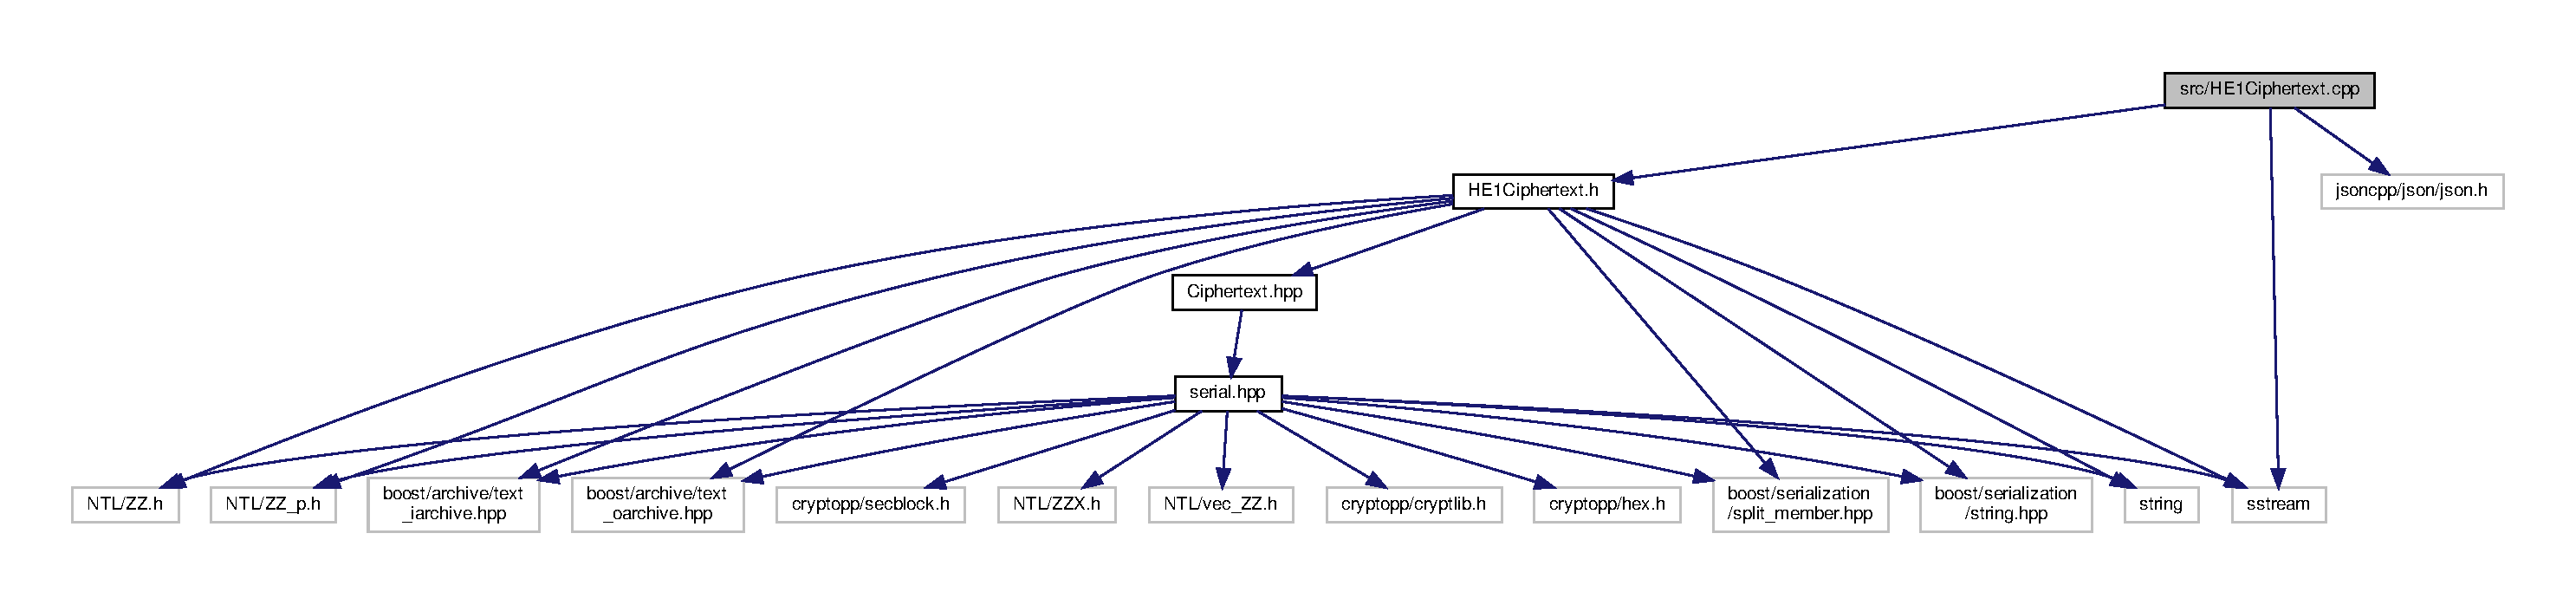
\includegraphics[width=350pt]{HE1Ciphertext_8cpp__incl}
\end{center}
\end{figure}
\subsection*{Functions}
\begin{DoxyCompactItemize}
\item 
std\+::ostream \& \hyperlink{HE1Ciphertext_8cpp_a684afdb22c43258ab0e2e5ab73abaed0}{operator$<$$<$} (std\+::ostream \&o, const \hyperlink{classHE1Ciphertext}{H\+E1\+Ciphertext} \&c)
\item 
\hyperlink{classHE1Ciphertext}{H\+E1\+Ciphertext} \hyperlink{HE1Ciphertext_8cpp_a2e914308f6b7d88f63067fca516f4055}{operator+} (const \hyperlink{classHE1Ciphertext}{H\+E1\+Ciphertext} \&a, const \hyperlink{classHE1Ciphertext}{H\+E1\+Ciphertext} \&b)
\item 
\hyperlink{classHE1Ciphertext}{H\+E1\+Ciphertext} \hyperlink{HE1Ciphertext_8cpp_a8b5554bdd70338b6c916db1423702314}{operator$\ast$} (const \hyperlink{classHE1Ciphertext}{H\+E1\+Ciphertext} \&a, const \hyperlink{classHE1Ciphertext}{H\+E1\+Ciphertext} \&b)
\end{DoxyCompactItemize}


\subsection{Function Documentation}
\mbox{\Hypertarget{HE1Ciphertext_8cpp_a8b5554bdd70338b6c916db1423702314}\label{HE1Ciphertext_8cpp_a8b5554bdd70338b6c916db1423702314}} 
\index{H\+E1\+Ciphertext.\+cpp@{H\+E1\+Ciphertext.\+cpp}!operator$\ast$@{operator$\ast$}}
\index{operator$\ast$@{operator$\ast$}!H\+E1\+Ciphertext.\+cpp@{H\+E1\+Ciphertext.\+cpp}}
\subsubsection{\texorpdfstring{operator$\ast$()}{operator*()}}
{\footnotesize\ttfamily \hyperlink{classHE1Ciphertext}{H\+E1\+Ciphertext} operator$\ast$ (\begin{DoxyParamCaption}\item[{const \hyperlink{classHE1Ciphertext}{H\+E1\+Ciphertext} \&}]{a,  }\item[{const \hyperlink{classHE1Ciphertext}{H\+E1\+Ciphertext} \&}]{b }\end{DoxyParamCaption})}

Performs modular multiplication of {\ttfamily a.\+ciphertext} and {\ttfamily b.\+ciphertext} 
\begin{DoxyParams}{Parameters}
{\em a} & {\ttfamily \hyperlink{classHE1Ciphertext}{H\+E1\+Ciphertext}} object \\
\hline
{\em b} & {\ttfamily \hyperlink{classHE1Ciphertext}{H\+E1\+Ciphertext}} object \\
\hline
\end{DoxyParams}
\begin{DoxyReturn}{Returns}
{\ttfamily \hyperlink{classHE1Ciphertext}{H\+E1\+Ciphertext}} object containing the product 
\end{DoxyReturn}
\mbox{\Hypertarget{HE1Ciphertext_8cpp_a2e914308f6b7d88f63067fca516f4055}\label{HE1Ciphertext_8cpp_a2e914308f6b7d88f63067fca516f4055}} 
\index{H\+E1\+Ciphertext.\+cpp@{H\+E1\+Ciphertext.\+cpp}!operator+@{operator+}}
\index{operator+@{operator+}!H\+E1\+Ciphertext.\+cpp@{H\+E1\+Ciphertext.\+cpp}}
\subsubsection{\texorpdfstring{operator+()}{operator+()}}
{\footnotesize\ttfamily \hyperlink{classHE1Ciphertext}{H\+E1\+Ciphertext} operator+ (\begin{DoxyParamCaption}\item[{const \hyperlink{classHE1Ciphertext}{H\+E1\+Ciphertext} \&}]{a,  }\item[{const \hyperlink{classHE1Ciphertext}{H\+E1\+Ciphertext} \&}]{b }\end{DoxyParamCaption})}

Performs modular addition of {\ttfamily a.\+ciphertext} and {\ttfamily b.\+ciphertext} 
\begin{DoxyParams}{Parameters}
{\em a} & {\ttfamily \hyperlink{classHE1Ciphertext}{H\+E1\+Ciphertext}} object \\
\hline
{\em b} & {\ttfamily \hyperlink{classHE1Ciphertext}{H\+E1\+Ciphertext}} object \\
\hline
\end{DoxyParams}
\begin{DoxyReturn}{Returns}
{\ttfamily \hyperlink{classHE1Ciphertext}{H\+E1\+Ciphertext}} object containing the sum 
\end{DoxyReturn}
\mbox{\Hypertarget{HE1Ciphertext_8cpp_a684afdb22c43258ab0e2e5ab73abaed0}\label{HE1Ciphertext_8cpp_a684afdb22c43258ab0e2e5ab73abaed0}} 
\index{H\+E1\+Ciphertext.\+cpp@{H\+E1\+Ciphertext.\+cpp}!operator$<$$<$@{operator$<$$<$}}
\index{operator$<$$<$@{operator$<$$<$}!H\+E1\+Ciphertext.\+cpp@{H\+E1\+Ciphertext.\+cpp}}
\subsubsection{\texorpdfstring{operator$<$$<$()}{operator<<()}}
{\footnotesize\ttfamily std\+::ostream\& operator$<$$<$ (\begin{DoxyParamCaption}\item[{std\+::ostream \&}]{o,  }\item[{const \hyperlink{classHE1Ciphertext}{H\+E1\+Ciphertext} \&}]{c }\end{DoxyParamCaption})}

Write {\ttfamily ciphertext} to output stream as decimal string 
\begin{DoxyParams}{Parameters}
{\em o} & Output stream \\
\hline
{\em c} & {\ttfamily \hyperlink{classHE1Ciphertext}{H\+E1\+Ciphertext}} object \\
\hline
\end{DoxyParams}
\begin{DoxyReturn}{Returns}
A reference to the output stream 
\end{DoxyReturn}

\hypertarget{HE2Ciphertext_8cpp}{}\section{src/\+H\+E2\+Ciphertext.cpp File Reference}
\label{HE2Ciphertext_8cpp}\index{src/\+H\+E2\+Ciphertext.\+cpp@{src/\+H\+E2\+Ciphertext.\+cpp}}
{\ttfamily \#include $<$jsoncpp/json/json.\+h$>$}\newline
{\ttfamily \#include \char`\"{}H\+E2\+Ciphertext.\+h\char`\"{}}\newline
Include dependency graph for H\+E2\+Ciphertext.\+cpp\+:
\nopagebreak
\begin{figure}[H]
\begin{center}
\leavevmode
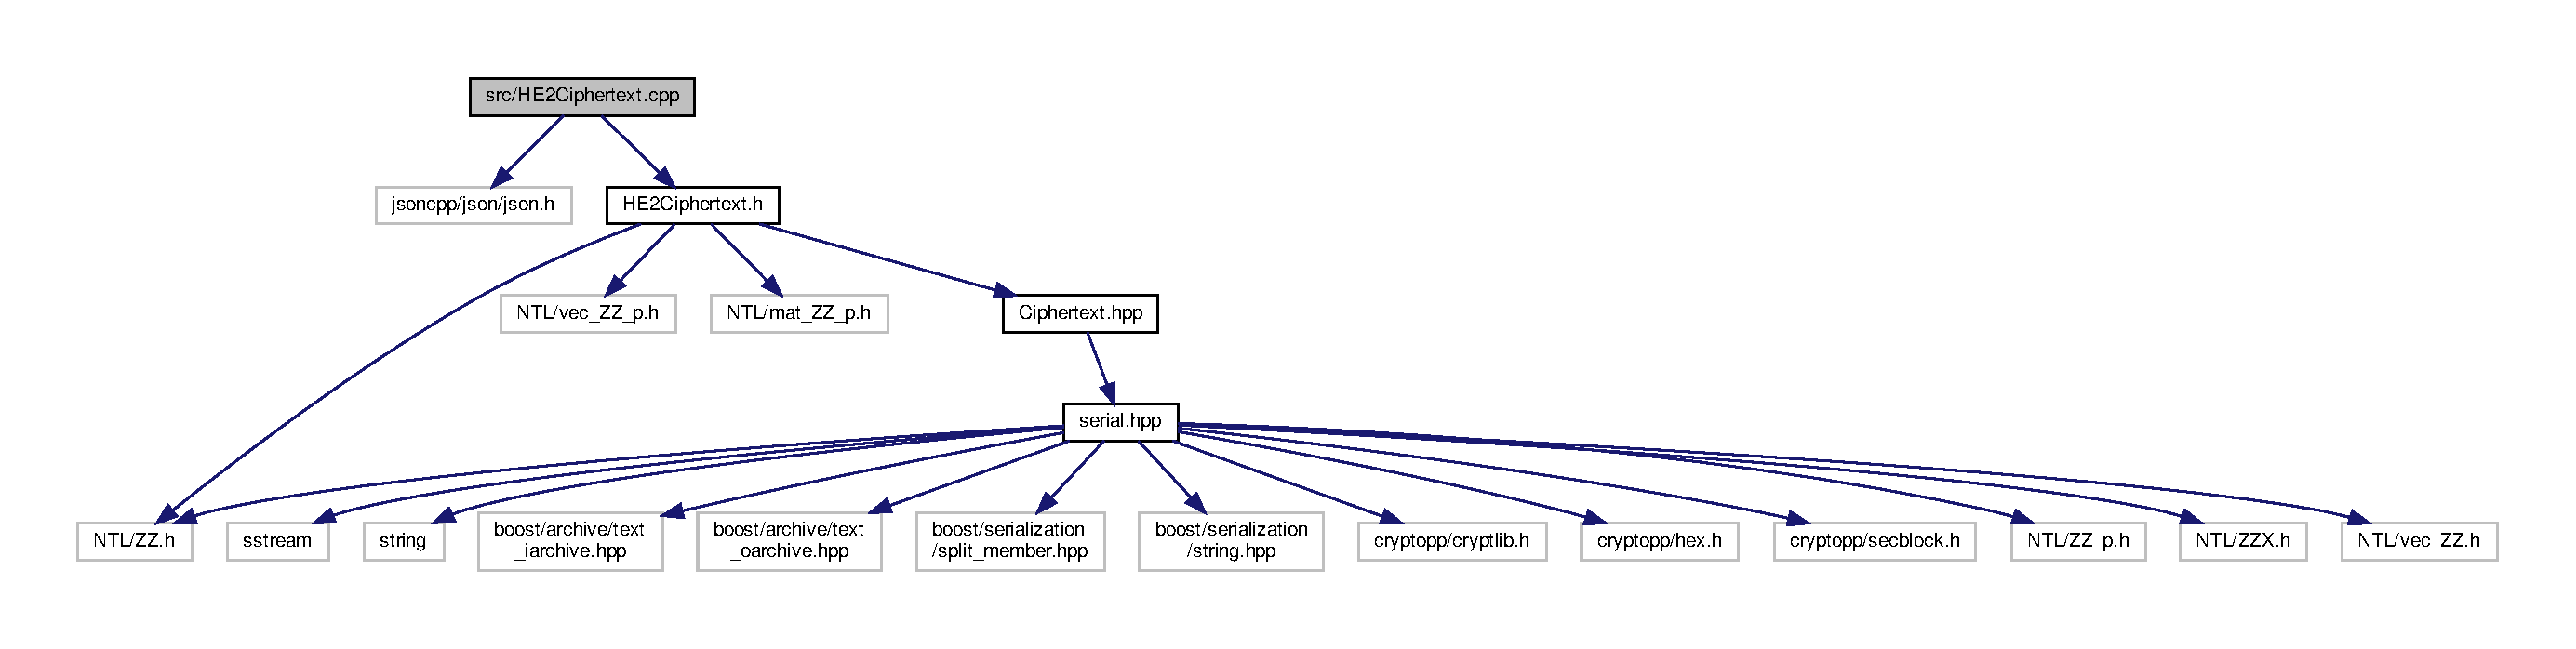
\includegraphics[width=350pt]{HE2Ciphertext_8cpp__incl}
\end{center}
\end{figure}
\subsection*{Functions}
\begin{DoxyCompactItemize}
\item 
std\+::ostream \& \hyperlink{HE2Ciphertext_8cpp_a5d9b4ffb87a447db8b95de9c64401e0f}{operator$<$$<$} (std\+::ostream \&o, const \hyperlink{classHE2Ciphertext}{H\+E2\+Ciphertext} \&c)
\item 
std\+::istream \& \hyperlink{HE2Ciphertext_8cpp_a8cd6e8f36f12e9b0548d6f66fae71816}{operator$>$$>$} (std\+::istream \&i, \hyperlink{classHE2Ciphertext}{H\+E2\+Ciphertext} \&c)
\item 
\hyperlink{classHE2Ciphertext}{H\+E2\+Ciphertext} \hyperlink{HE2Ciphertext_8cpp_af90fd206e69fa74b30d40f41f707bdb8}{operator+} (const \hyperlink{classHE2Ciphertext}{H\+E2\+Ciphertext} \&a, const \hyperlink{classHE2Ciphertext}{H\+E2\+Ciphertext} \&b)
\item 
\hyperlink{classHE2Ciphertext}{H\+E2\+Ciphertext} \hyperlink{HE2Ciphertext_8cpp_adfb636b8ce661b0edbd9297cdcf61c88}{operator$\ast$} (const \hyperlink{classHE2Ciphertext}{H\+E2\+Ciphertext} \&a, const \hyperlink{classHE2Ciphertext}{H\+E2\+Ciphertext} \&b)
\end{DoxyCompactItemize}


\subsection{Function Documentation}
\mbox{\Hypertarget{HE2Ciphertext_8cpp_adfb636b8ce661b0edbd9297cdcf61c88}\label{HE2Ciphertext_8cpp_adfb636b8ce661b0edbd9297cdcf61c88}} 
\index{H\+E2\+Ciphertext.\+cpp@{H\+E2\+Ciphertext.\+cpp}!operator$\ast$@{operator$\ast$}}
\index{operator$\ast$@{operator$\ast$}!H\+E2\+Ciphertext.\+cpp@{H\+E2\+Ciphertext.\+cpp}}
\subsubsection{\texorpdfstring{operator$\ast$()}{operator*()}}
{\footnotesize\ttfamily \hyperlink{classHE2Ciphertext}{H\+E2\+Ciphertext} operator$\ast$ (\begin{DoxyParamCaption}\item[{const \hyperlink{classHE2Ciphertext}{H\+E2\+Ciphertext} \&}]{a,  }\item[{const \hyperlink{classHE2Ciphertext}{H\+E2\+Ciphertext} \&}]{b }\end{DoxyParamCaption})}

Multiplies the {\ttfamily ciphertexts} of each object. In the context of the H\+E2 ciphers, multiplication is the Hadamard product of augmented vectors, followed by multiplication by the matrix {\ttfamily R}. \begin{DoxySeeAlso}{See also}
product 

augment 
\end{DoxySeeAlso}

\begin{DoxyParams}{Parameters}
{\em a} & An {\ttfamily \hyperlink{classHE2Ciphertext}{H\+E2\+Ciphertext}} object \\
\hline
{\em b} & An {\ttfamily \hyperlink{classHE2Ciphertext}{H\+E2\+Ciphertext}} object \\
\hline
\end{DoxyParams}
\begin{DoxyReturn}{Returns}
A new {\ttfamily \hyperlink{classHE2Ciphertext}{H\+E2\+Ciphertext}} object containing the sum 
\end{DoxyReturn}
\mbox{\Hypertarget{HE2Ciphertext_8cpp_af90fd206e69fa74b30d40f41f707bdb8}\label{HE2Ciphertext_8cpp_af90fd206e69fa74b30d40f41f707bdb8}} 
\index{H\+E2\+Ciphertext.\+cpp@{H\+E2\+Ciphertext.\+cpp}!operator+@{operator+}}
\index{operator+@{operator+}!H\+E2\+Ciphertext.\+cpp@{H\+E2\+Ciphertext.\+cpp}}
\subsubsection{\texorpdfstring{operator+()}{operator+()}}
{\footnotesize\ttfamily \hyperlink{classHE2Ciphertext}{H\+E2\+Ciphertext} operator+ (\begin{DoxyParamCaption}\item[{const \hyperlink{classHE2Ciphertext}{H\+E2\+Ciphertext} \&}]{a,  }\item[{const \hyperlink{classHE2Ciphertext}{H\+E2\+Ciphertext} \&}]{b }\end{DoxyParamCaption})}

Add the {\ttfamily ciphertexts} of each object 
\begin{DoxyParams}{Parameters}
{\em a} & An {\ttfamily \hyperlink{classHE2Ciphertext}{H\+E2\+Ciphertext}} object \\
\hline
{\em b} & An {\ttfamily \hyperlink{classHE2Ciphertext}{H\+E2\+Ciphertext}} object \\
\hline
\end{DoxyParams}
\begin{DoxyReturn}{Returns}
A new {\ttfamily \hyperlink{classHE2Ciphertext}{H\+E2\+Ciphertext}} object containing the sum 
\end{DoxyReturn}
\mbox{\Hypertarget{HE2Ciphertext_8cpp_a5d9b4ffb87a447db8b95de9c64401e0f}\label{HE2Ciphertext_8cpp_a5d9b4ffb87a447db8b95de9c64401e0f}} 
\index{H\+E2\+Ciphertext.\+cpp@{H\+E2\+Ciphertext.\+cpp}!operator$<$$<$@{operator$<$$<$}}
\index{operator$<$$<$@{operator$<$$<$}!H\+E2\+Ciphertext.\+cpp@{H\+E2\+Ciphertext.\+cpp}}
\subsubsection{\texorpdfstring{operator$<$$<$()}{operator<<()}}
{\footnotesize\ttfamily std\+::ostream\& operator$<$$<$ (\begin{DoxyParamCaption}\item[{std\+::ostream \&}]{o,  }\item[{const \hyperlink{classHE2Ciphertext}{H\+E2\+Ciphertext} \&}]{c }\end{DoxyParamCaption})}

Write the {\ttfamily ciphertext} to a stream 
\begin{DoxyParams}{Parameters}
{\em o} & An output stream \\
\hline
{\em c} & A {\ttfamily \hyperlink{classHE2Ciphertext}{H\+E2\+Ciphertext}} object \\
\hline
\end{DoxyParams}
\begin{DoxyReturn}{Returns}
A reference to the output stream 
\end{DoxyReturn}
\mbox{\Hypertarget{HE2Ciphertext_8cpp_a8cd6e8f36f12e9b0548d6f66fae71816}\label{HE2Ciphertext_8cpp_a8cd6e8f36f12e9b0548d6f66fae71816}} 
\index{H\+E2\+Ciphertext.\+cpp@{H\+E2\+Ciphertext.\+cpp}!operator$>$$>$@{operator$>$$>$}}
\index{operator$>$$>$@{operator$>$$>$}!H\+E2\+Ciphertext.\+cpp@{H\+E2\+Ciphertext.\+cpp}}
\subsubsection{\texorpdfstring{operator$>$$>$()}{operator>>()}}
{\footnotesize\ttfamily std\+::istream\& operator$>$$>$ (\begin{DoxyParamCaption}\item[{std\+::istream \&}]{i,  }\item[{\hyperlink{classHE2Ciphertext}{H\+E2\+Ciphertext} \&}]{c }\end{DoxyParamCaption})}

Read the {\ttfamily ciphertext} from an input stream 
\begin{DoxyParams}{Parameters}
{\em i} & An input stream \\
\hline
{\em c} & A {\ttfamily \hyperlink{classHE2Ciphertext}{H\+E2\+Ciphertext}} object \\
\hline
\end{DoxyParams}
\begin{DoxyReturn}{Returns}
A reference to the output stream 
\end{DoxyReturn}

\hypertarget{OPECiphertext_8cpp}{}\section{src/\+O\+P\+E\+Ciphertext.cpp File Reference}
\label{OPECiphertext_8cpp}\index{src/\+O\+P\+E\+Ciphertext.\+cpp@{src/\+O\+P\+E\+Ciphertext.\+cpp}}
{\ttfamily \#include \char`\"{}O\+P\+E\+Ciphertext.\+h\char`\"{}}\newline
Include dependency graph for O\+P\+E\+Ciphertext.\+cpp\+:
\nopagebreak
\begin{figure}[H]
\begin{center}
\leavevmode
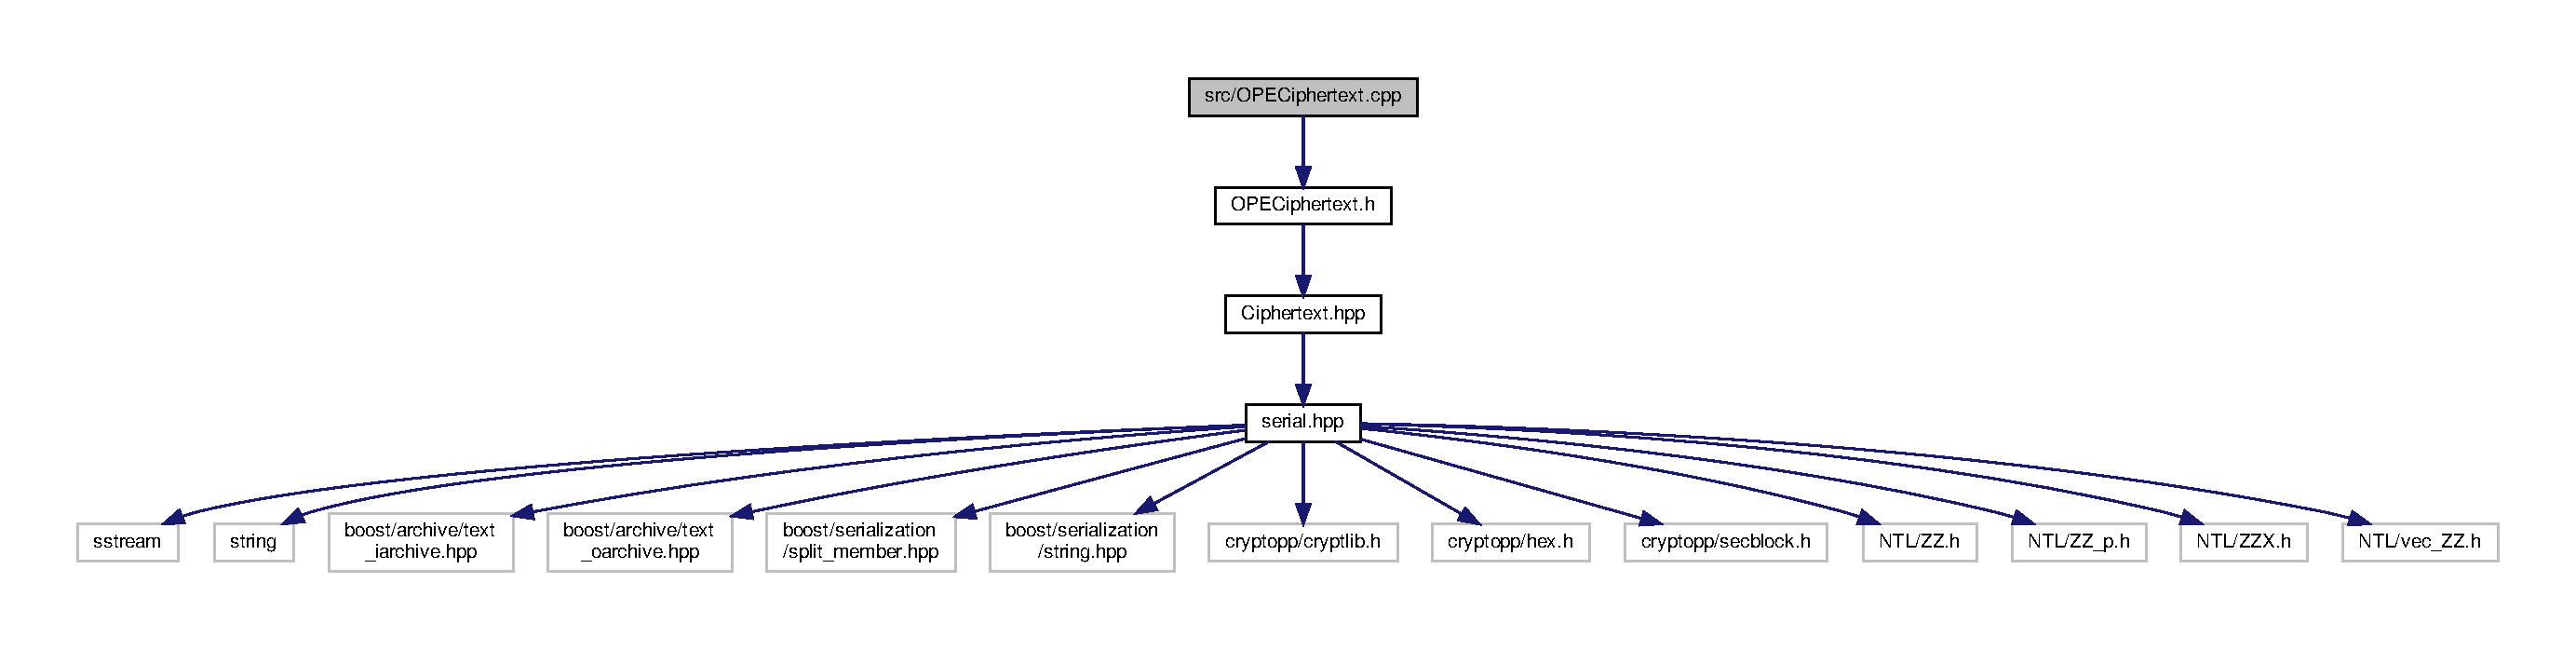
\includegraphics[width=350pt]{OPECiphertext_8cpp__incl}
\end{center}
\end{figure}
\subsection*{Functions}
\begin{DoxyCompactItemize}
\item 
std\+::ostream \& \hyperlink{OPECiphertext_8cpp_acbdbfe3a8b342ed91b375a30c19423a3}{operator$<$$<$} (std\+::ostream \&o, const \hyperlink{classOPECiphertext}{O\+P\+E\+Ciphertext} \&c)
\item 
std\+::istream \& \hyperlink{OPECiphertext_8cpp_a78faeb1ac9b11d0aa4337957b9fba288}{operator$>$$>$} (std\+::istream \&i, \hyperlink{classOPECiphertext}{O\+P\+E\+Ciphertext} \&c)
\item 
bool \hyperlink{OPECiphertext_8cpp_a7a856f70b6a7c9c384e5bcc59d4665ca}{operator$<$} (const \hyperlink{classOPECiphertext}{O\+P\+E\+Ciphertext} \&a, const \hyperlink{classOPECiphertext}{O\+P\+E\+Ciphertext} \&b)
\item 
bool \hyperlink{OPECiphertext_8cpp_a6e3f45959b24805b5e007867bde5ac52}{operator$<$=} (const \hyperlink{classOPECiphertext}{O\+P\+E\+Ciphertext} \&a, const \hyperlink{classOPECiphertext}{O\+P\+E\+Ciphertext} \&b)
\item 
bool \hyperlink{OPECiphertext_8cpp_a434a85cf1acb2e87f59cb598aa67aac1}{operator==} (const \hyperlink{classOPECiphertext}{O\+P\+E\+Ciphertext} \&a, const \hyperlink{classOPECiphertext}{O\+P\+E\+Ciphertext} \&b)
\item 
bool \hyperlink{OPECiphertext_8cpp_a5a05c9bf39f65f099132a4cb3c030fc0}{operator$>$} (const \hyperlink{classOPECiphertext}{O\+P\+E\+Ciphertext} \&a, const \hyperlink{classOPECiphertext}{O\+P\+E\+Ciphertext} \&b)
\item 
bool \hyperlink{OPECiphertext_8cpp_a2e7887e9daea66096a9526a493cdc023}{operator$>$=} (const \hyperlink{classOPECiphertext}{O\+P\+E\+Ciphertext} \&a, const \hyperlink{classOPECiphertext}{O\+P\+E\+Ciphertext} \&b)
\end{DoxyCompactItemize}


\subsection{Function Documentation}
\mbox{\Hypertarget{OPECiphertext_8cpp_a7a856f70b6a7c9c384e5bcc59d4665ca}\label{OPECiphertext_8cpp_a7a856f70b6a7c9c384e5bcc59d4665ca}} 
\index{O\+P\+E\+Ciphertext.\+cpp@{O\+P\+E\+Ciphertext.\+cpp}!operator$<$@{operator$<$}}
\index{operator$<$@{operator$<$}!O\+P\+E\+Ciphertext.\+cpp@{O\+P\+E\+Ciphertext.\+cpp}}
\subsubsection{\texorpdfstring{operator$<$()}{operator<()}}
{\footnotesize\ttfamily bool operator$<$ (\begin{DoxyParamCaption}\item[{const \hyperlink{classOPECiphertext}{O\+P\+E\+Ciphertext} \&}]{a,  }\item[{const \hyperlink{classOPECiphertext}{O\+P\+E\+Ciphertext} \&}]{b }\end{DoxyParamCaption})}

Returns {\ttfamily a.\+ciphertext} $<$ {\ttfamily b.\+ciphertext} 
\begin{DoxyParams}{Parameters}
{\em a} & {\ttfamily \hyperlink{classOPECiphertext}{O\+P\+E\+Ciphertext}} object \\
\hline
{\em b} & {\ttfamily \hyperlink{classOPECiphertext}{O\+P\+E\+Ciphertext}} object \\
\hline
\end{DoxyParams}
\begin{DoxyReturn}{Returns}
{\ttfamily true} or {\ttfamily false} 
\end{DoxyReturn}
\mbox{\Hypertarget{OPECiphertext_8cpp_acbdbfe3a8b342ed91b375a30c19423a3}\label{OPECiphertext_8cpp_acbdbfe3a8b342ed91b375a30c19423a3}} 
\index{O\+P\+E\+Ciphertext.\+cpp@{O\+P\+E\+Ciphertext.\+cpp}!operator$<$$<$@{operator$<$$<$}}
\index{operator$<$$<$@{operator$<$$<$}!O\+P\+E\+Ciphertext.\+cpp@{O\+P\+E\+Ciphertext.\+cpp}}
\subsubsection{\texorpdfstring{operator$<$$<$()}{operator<<()}}
{\footnotesize\ttfamily std\+::ostream\& operator$<$$<$ (\begin{DoxyParamCaption}\item[{std\+::ostream \&}]{o,  }\item[{const \hyperlink{classOPECiphertext}{O\+P\+E\+Ciphertext} \&}]{c }\end{DoxyParamCaption})}

Write {\ttfamily ciphertext} as decimal string to the output stream 
\begin{DoxyParams}{Parameters}
{\em o} & Output stream \\
\hline
{\em c} & {\ttfamily \hyperlink{classOPECiphertext}{O\+P\+E\+Ciphertext}} object \\
\hline
\end{DoxyParams}
\begin{DoxyReturn}{Returns}
a reference to the output stream 
\end{DoxyReturn}
\mbox{\Hypertarget{OPECiphertext_8cpp_a6e3f45959b24805b5e007867bde5ac52}\label{OPECiphertext_8cpp_a6e3f45959b24805b5e007867bde5ac52}} 
\index{O\+P\+E\+Ciphertext.\+cpp@{O\+P\+E\+Ciphertext.\+cpp}!operator$<$=@{operator$<$=}}
\index{operator$<$=@{operator$<$=}!O\+P\+E\+Ciphertext.\+cpp@{O\+P\+E\+Ciphertext.\+cpp}}
\subsubsection{\texorpdfstring{operator$<$=()}{operator<=()}}
{\footnotesize\ttfamily bool operator$<$= (\begin{DoxyParamCaption}\item[{const \hyperlink{classOPECiphertext}{O\+P\+E\+Ciphertext} \&}]{a,  }\item[{const \hyperlink{classOPECiphertext}{O\+P\+E\+Ciphertext} \&}]{b }\end{DoxyParamCaption})}

Returns {\ttfamily a.\+ciphertext} {$\le$} {\ttfamily b.\+ciphertext} 
\begin{DoxyParams}{Parameters}
{\em a} & {\ttfamily \hyperlink{classOPECiphertext}{O\+P\+E\+Ciphertext}} object \\
\hline
{\em b} & {\ttfamily \hyperlink{classOPECiphertext}{O\+P\+E\+Ciphertext}} object \\
\hline
\end{DoxyParams}
\begin{DoxyReturn}{Returns}
{\ttfamily true} or {\ttfamily false} 
\end{DoxyReturn}
\mbox{\Hypertarget{OPECiphertext_8cpp_a434a85cf1acb2e87f59cb598aa67aac1}\label{OPECiphertext_8cpp_a434a85cf1acb2e87f59cb598aa67aac1}} 
\index{O\+P\+E\+Ciphertext.\+cpp@{O\+P\+E\+Ciphertext.\+cpp}!operator==@{operator==}}
\index{operator==@{operator==}!O\+P\+E\+Ciphertext.\+cpp@{O\+P\+E\+Ciphertext.\+cpp}}
\subsubsection{\texorpdfstring{operator==()}{operator==()}}
{\footnotesize\ttfamily bool operator== (\begin{DoxyParamCaption}\item[{const \hyperlink{classOPECiphertext}{O\+P\+E\+Ciphertext} \&}]{a,  }\item[{const \hyperlink{classOPECiphertext}{O\+P\+E\+Ciphertext} \&}]{b }\end{DoxyParamCaption})}

Returns {\ttfamily a.\+ciphertext} = {\ttfamily b.\+ciphertext} 
\begin{DoxyParams}{Parameters}
{\em a} & {\ttfamily \hyperlink{classOPECiphertext}{O\+P\+E\+Ciphertext}} object \\
\hline
{\em b} & {\ttfamily \hyperlink{classOPECiphertext}{O\+P\+E\+Ciphertext}} object \\
\hline
\end{DoxyParams}
\begin{DoxyReturn}{Returns}
{\ttfamily true} or {\ttfamily false} 
\end{DoxyReturn}
\mbox{\Hypertarget{OPECiphertext_8cpp_a5a05c9bf39f65f099132a4cb3c030fc0}\label{OPECiphertext_8cpp_a5a05c9bf39f65f099132a4cb3c030fc0}} 
\index{O\+P\+E\+Ciphertext.\+cpp@{O\+P\+E\+Ciphertext.\+cpp}!operator$>$@{operator$>$}}
\index{operator$>$@{operator$>$}!O\+P\+E\+Ciphertext.\+cpp@{O\+P\+E\+Ciphertext.\+cpp}}
\subsubsection{\texorpdfstring{operator$>$()}{operator>()}}
{\footnotesize\ttfamily bool operator$>$ (\begin{DoxyParamCaption}\item[{const \hyperlink{classOPECiphertext}{O\+P\+E\+Ciphertext} \&}]{a,  }\item[{const \hyperlink{classOPECiphertext}{O\+P\+E\+Ciphertext} \&}]{b }\end{DoxyParamCaption})}

Returns {\ttfamily a.\+ciphertext} $>$ {\ttfamily b.\+ciphertext} 
\begin{DoxyParams}{Parameters}
{\em a} & {\ttfamily \hyperlink{classOPECiphertext}{O\+P\+E\+Ciphertext}} object \\
\hline
{\em b} & {\ttfamily \hyperlink{classOPECiphertext}{O\+P\+E\+Ciphertext}} object \\
\hline
\end{DoxyParams}
\begin{DoxyReturn}{Returns}
{\ttfamily true} or {\ttfamily false} 
\end{DoxyReturn}
\mbox{\Hypertarget{OPECiphertext_8cpp_a2e7887e9daea66096a9526a493cdc023}\label{OPECiphertext_8cpp_a2e7887e9daea66096a9526a493cdc023}} 
\index{O\+P\+E\+Ciphertext.\+cpp@{O\+P\+E\+Ciphertext.\+cpp}!operator$>$=@{operator$>$=}}
\index{operator$>$=@{operator$>$=}!O\+P\+E\+Ciphertext.\+cpp@{O\+P\+E\+Ciphertext.\+cpp}}
\subsubsection{\texorpdfstring{operator$>$=()}{operator>=()}}
{\footnotesize\ttfamily bool operator$>$= (\begin{DoxyParamCaption}\item[{const \hyperlink{classOPECiphertext}{O\+P\+E\+Ciphertext} \&}]{a,  }\item[{const \hyperlink{classOPECiphertext}{O\+P\+E\+Ciphertext} \&}]{b }\end{DoxyParamCaption})}

Returns {\ttfamily a.\+ciphertext} {$\ge$} {\ttfamily b.\+ciphertext} 
\begin{DoxyParams}{Parameters}
{\em a} & {\ttfamily \hyperlink{classOPECiphertext}{O\+P\+E\+Ciphertext}} object \\
\hline
{\em b} & {\ttfamily \hyperlink{classOPECiphertext}{O\+P\+E\+Ciphertext}} object \\
\hline
\end{DoxyParams}
\begin{DoxyReturn}{Returns}
{\ttfamily true} or {\ttfamily false} 
\end{DoxyReturn}
\mbox{\Hypertarget{OPECiphertext_8cpp_a78faeb1ac9b11d0aa4337957b9fba288}\label{OPECiphertext_8cpp_a78faeb1ac9b11d0aa4337957b9fba288}} 
\index{O\+P\+E\+Ciphertext.\+cpp@{O\+P\+E\+Ciphertext.\+cpp}!operator$>$$>$@{operator$>$$>$}}
\index{operator$>$$>$@{operator$>$$>$}!O\+P\+E\+Ciphertext.\+cpp@{O\+P\+E\+Ciphertext.\+cpp}}
\subsubsection{\texorpdfstring{operator$>$$>$()}{operator>>()}}
{\footnotesize\ttfamily std\+::istream\& operator$>$$>$ (\begin{DoxyParamCaption}\item[{std\+::istream \&}]{i,  }\item[{\hyperlink{classOPECiphertext}{O\+P\+E\+Ciphertext} \&}]{c }\end{DoxyParamCaption})}

Read {\ttfamily ciphertext} as decimal string from the input stream and convert to {\ttfamily N\+T\+L\+::\+ZZ} 
\begin{DoxyParams}{Parameters}
{\em i} & Input stream \\
\hline
{\em c} & {\ttfamily \hyperlink{classOPECiphertext}{O\+P\+E\+Ciphertext}} object \\
\hline
\end{DoxyParams}
\begin{DoxyReturn}{Returns}
a reference to the output stream 
\end{DoxyReturn}

\hypertarget{PolyCiphertext_8cpp}{}\section{src/\+Poly\+Ciphertext.cpp File Reference}
\label{PolyCiphertext_8cpp}\index{src/\+Poly\+Ciphertext.\+cpp@{src/\+Poly\+Ciphertext.\+cpp}}
{\ttfamily \#include \char`\"{}Poly\+Ciphertext.\+h\char`\"{}}\newline
{\ttfamily \#include $<$iostream$>$}\newline
{\ttfamily \#include $<$sstream$>$}\newline
{\ttfamily \#include $<$string$>$}\newline
Include dependency graph for Poly\+Ciphertext.\+cpp\+:
\nopagebreak
\begin{figure}[H]
\begin{center}
\leavevmode
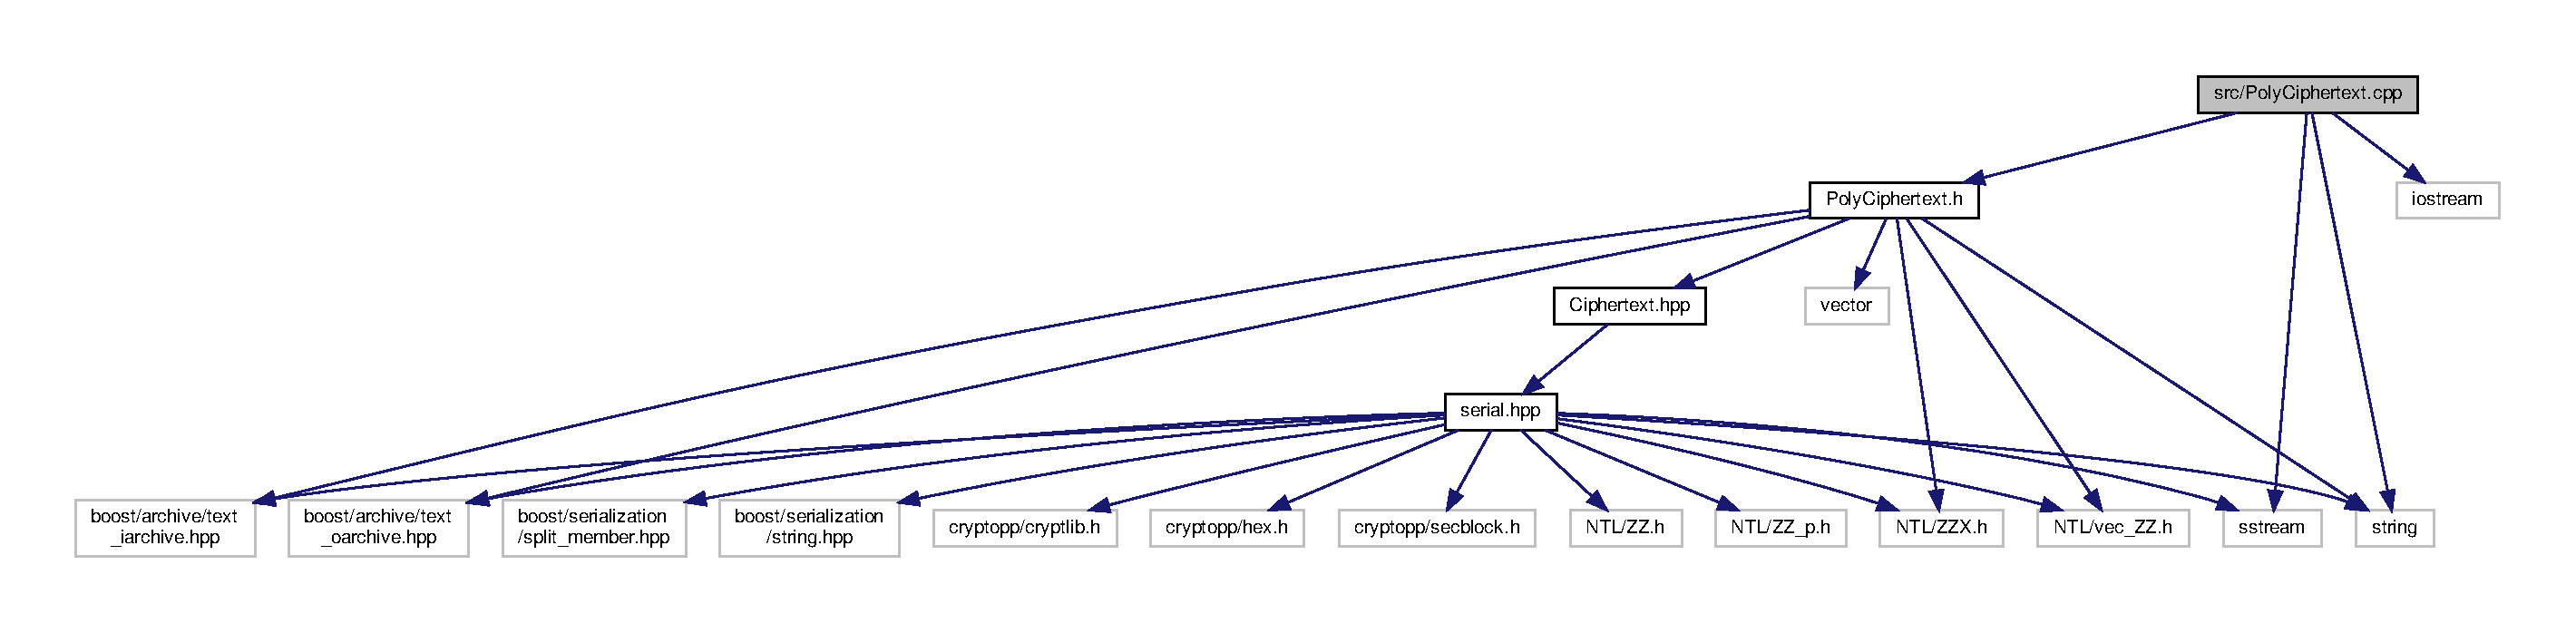
\includegraphics[width=350pt]{PolyCiphertext_8cpp__incl}
\end{center}
\end{figure}
\subsection*{Functions}
\begin{DoxyCompactItemize}
\item 
int \hyperlink{PolyCiphertext_8cpp_a2a25d0399b812261d703d84fd3a21fb9}{compare} (const \hyperlink{classPolyCiphertext}{Poly\+Ciphertext} \&a, const \hyperlink{classPolyCiphertext}{Poly\+Ciphertext} \&b)
\item 
bool \hyperlink{PolyCiphertext_8cpp_ab5a64cd27170239ff233b1a17f5b0de9}{operator$<$} (const \hyperlink{classPolyCiphertext}{Poly\+Ciphertext} \&a, const \hyperlink{classPolyCiphertext}{Poly\+Ciphertext} \&b)
\item 
bool \hyperlink{PolyCiphertext_8cpp_a3199ddbed52caee0d591894b60389144}{operator$<$=} (const \hyperlink{classPolyCiphertext}{Poly\+Ciphertext} \&a, const \hyperlink{classPolyCiphertext}{Poly\+Ciphertext} \&b)
\item 
bool \hyperlink{PolyCiphertext_8cpp_a441251a147b7c15eccf64048ba9fb0fe}{operator==} (const \hyperlink{classPolyCiphertext}{Poly\+Ciphertext} \&a, const \hyperlink{classPolyCiphertext}{Poly\+Ciphertext} \&b)
\item 
bool \hyperlink{PolyCiphertext_8cpp_a2a58b35102feabe6b31bacdd457d7884}{operator$>$} (const \hyperlink{classPolyCiphertext}{Poly\+Ciphertext} \&a, const \hyperlink{classPolyCiphertext}{Poly\+Ciphertext} \&b)
\item 
bool \hyperlink{PolyCiphertext_8cpp_ab76ec0162c70ea00a11f921d617d102d}{operator$>$=} (const \hyperlink{classPolyCiphertext}{Poly\+Ciphertext} \&a, const \hyperlink{classPolyCiphertext}{Poly\+Ciphertext} \&b)
\end{DoxyCompactItemize}


\subsection{Function Documentation}
\mbox{\Hypertarget{PolyCiphertext_8cpp_a2a25d0399b812261d703d84fd3a21fb9}\label{PolyCiphertext_8cpp_a2a25d0399b812261d703d84fd3a21fb9}} 
\index{Poly\+Ciphertext.\+cpp@{Poly\+Ciphertext.\+cpp}!compare@{compare}}
\index{compare@{compare}!Poly\+Ciphertext.\+cpp@{Poly\+Ciphertext.\+cpp}}
\subsubsection{\texorpdfstring{compare()}{compare()}}
{\footnotesize\ttfamily int compare (\begin{DoxyParamCaption}\item[{const \hyperlink{classPolyCiphertext}{Poly\+Ciphertext} \&}]{a,  }\item[{const \hyperlink{classPolyCiphertext}{Poly\+Ciphertext} \&}]{b }\end{DoxyParamCaption})}

Auxiliary function to compare two polynomials lexicographically (a polynomial of larger degree is considered to be ordered higher than a lower degree polynomial). Returns -\/1 is {\ttfamily a.\+ciphertext} $<$ {\ttfamily b.\+ciphertext}, 0 if {\ttfamily a.\+ciphertext} = {\ttfamily b.\+ciphertext}, and 1 if {\ttfamily a.\+ciphertext} $>$ {\ttfamily b.\+ciphertext} 
\begin{DoxyParams}{Parameters}
{\em a} & A {\ttfamily \hyperlink{classPolyCiphertext}{Poly\+Ciphertext}} object \\
\hline
{\em b} & A {\ttfamily \hyperlink{classPolyCiphertext}{Poly\+Ciphertext}} object \\
\hline
\end{DoxyParams}
\begin{DoxyReturn}{Returns}
-\/1, 0, or 1 
\end{DoxyReturn}
\mbox{\Hypertarget{PolyCiphertext_8cpp_ab5a64cd27170239ff233b1a17f5b0de9}\label{PolyCiphertext_8cpp_ab5a64cd27170239ff233b1a17f5b0de9}} 
\index{Poly\+Ciphertext.\+cpp@{Poly\+Ciphertext.\+cpp}!operator$<$@{operator$<$}}
\index{operator$<$@{operator$<$}!Poly\+Ciphertext.\+cpp@{Poly\+Ciphertext.\+cpp}}
\subsubsection{\texorpdfstring{operator$<$()}{operator<()}}
{\footnotesize\ttfamily bool operator$<$ (\begin{DoxyParamCaption}\item[{const \hyperlink{classPolyCiphertext}{Poly\+Ciphertext} \&}]{a,  }\item[{const \hyperlink{classPolyCiphertext}{Poly\+Ciphertext} \&}]{b }\end{DoxyParamCaption})}

Returns true if {\ttfamily a.\+ciphertext} is strictly less than {\ttfamily b.\+ciphertext} 
\begin{DoxyParams}{Parameters}
{\em a} & A {\ttfamily \hyperlink{classPolyCiphertext}{Poly\+Ciphertext}} object \\
\hline
{\em b} & A {\ttfamily \hyperlink{classPolyCiphertext}{Poly\+Ciphertext}} object \\
\hline
\end{DoxyParams}
\begin{DoxyReturn}{Returns}
{\ttfamily true} or {\ttfamily false} 
\end{DoxyReturn}
\mbox{\Hypertarget{PolyCiphertext_8cpp_a3199ddbed52caee0d591894b60389144}\label{PolyCiphertext_8cpp_a3199ddbed52caee0d591894b60389144}} 
\index{Poly\+Ciphertext.\+cpp@{Poly\+Ciphertext.\+cpp}!operator$<$=@{operator$<$=}}
\index{operator$<$=@{operator$<$=}!Poly\+Ciphertext.\+cpp@{Poly\+Ciphertext.\+cpp}}
\subsubsection{\texorpdfstring{operator$<$=()}{operator<=()}}
{\footnotesize\ttfamily bool operator$<$= (\begin{DoxyParamCaption}\item[{const \hyperlink{classPolyCiphertext}{Poly\+Ciphertext} \&}]{a,  }\item[{const \hyperlink{classPolyCiphertext}{Poly\+Ciphertext} \&}]{b }\end{DoxyParamCaption})}

Returns true if {\ttfamily a.\+ciphertext} is less than or equal to {\ttfamily b.\+ciphertext} 
\begin{DoxyParams}{Parameters}
{\em a} & A {\ttfamily \hyperlink{classPolyCiphertext}{Poly\+Ciphertext}} object \\
\hline
{\em b} & A {\ttfamily \hyperlink{classPolyCiphertext}{Poly\+Ciphertext}} object \\
\hline
\end{DoxyParams}
\begin{DoxyReturn}{Returns}
{\ttfamily true} or {\ttfamily false} 
\end{DoxyReturn}
\mbox{\Hypertarget{PolyCiphertext_8cpp_a441251a147b7c15eccf64048ba9fb0fe}\label{PolyCiphertext_8cpp_a441251a147b7c15eccf64048ba9fb0fe}} 
\index{Poly\+Ciphertext.\+cpp@{Poly\+Ciphertext.\+cpp}!operator==@{operator==}}
\index{operator==@{operator==}!Poly\+Ciphertext.\+cpp@{Poly\+Ciphertext.\+cpp}}
\subsubsection{\texorpdfstring{operator==()}{operator==()}}
{\footnotesize\ttfamily bool operator== (\begin{DoxyParamCaption}\item[{const \hyperlink{classPolyCiphertext}{Poly\+Ciphertext} \&}]{a,  }\item[{const \hyperlink{classPolyCiphertext}{Poly\+Ciphertext} \&}]{b }\end{DoxyParamCaption})}

Returns true if {\ttfamily a.\+ciphertext} is equal to {\ttfamily b.\+ciphertext} 
\begin{DoxyParams}{Parameters}
{\em a} & A {\ttfamily \hyperlink{classPolyCiphertext}{Poly\+Ciphertext}} object \\
\hline
{\em b} & A {\ttfamily \hyperlink{classPolyCiphertext}{Poly\+Ciphertext}} object \\
\hline
\end{DoxyParams}
\begin{DoxyReturn}{Returns}
{\ttfamily true} or {\ttfamily false} 
\end{DoxyReturn}
\mbox{\Hypertarget{PolyCiphertext_8cpp_a2a58b35102feabe6b31bacdd457d7884}\label{PolyCiphertext_8cpp_a2a58b35102feabe6b31bacdd457d7884}} 
\index{Poly\+Ciphertext.\+cpp@{Poly\+Ciphertext.\+cpp}!operator$>$@{operator$>$}}
\index{operator$>$@{operator$>$}!Poly\+Ciphertext.\+cpp@{Poly\+Ciphertext.\+cpp}}
\subsubsection{\texorpdfstring{operator$>$()}{operator>()}}
{\footnotesize\ttfamily bool operator$>$ (\begin{DoxyParamCaption}\item[{const \hyperlink{classPolyCiphertext}{Poly\+Ciphertext} \&}]{a,  }\item[{const \hyperlink{classPolyCiphertext}{Poly\+Ciphertext} \&}]{b }\end{DoxyParamCaption})}

Returns true if {\ttfamily a.\+ciphertext} is greater than {\ttfamily b.\+ciphertext} 
\begin{DoxyParams}{Parameters}
{\em a} & A {\ttfamily \hyperlink{classPolyCiphertext}{Poly\+Ciphertext}} object \\
\hline
{\em b} & A {\ttfamily \hyperlink{classPolyCiphertext}{Poly\+Ciphertext}} object \\
\hline
\end{DoxyParams}
\begin{DoxyReturn}{Returns}
{\ttfamily true} or {\ttfamily false} 
\end{DoxyReturn}
\mbox{\Hypertarget{PolyCiphertext_8cpp_ab76ec0162c70ea00a11f921d617d102d}\label{PolyCiphertext_8cpp_ab76ec0162c70ea00a11f921d617d102d}} 
\index{Poly\+Ciphertext.\+cpp@{Poly\+Ciphertext.\+cpp}!operator$>$=@{operator$>$=}}
\index{operator$>$=@{operator$>$=}!Poly\+Ciphertext.\+cpp@{Poly\+Ciphertext.\+cpp}}
\subsubsection{\texorpdfstring{operator$>$=()}{operator>=()}}
{\footnotesize\ttfamily bool operator$>$= (\begin{DoxyParamCaption}\item[{const \hyperlink{classPolyCiphertext}{Poly\+Ciphertext} \&}]{a,  }\item[{const \hyperlink{classPolyCiphertext}{Poly\+Ciphertext} \&}]{b }\end{DoxyParamCaption})}

Returns true if {\ttfamily a.\+ciphertext} is greater than or equal to {\ttfamily b.\+ciphertext} 
\begin{DoxyParams}{Parameters}
{\em a} & A {\ttfamily \hyperlink{classPolyCiphertext}{Poly\+Ciphertext}} object \\
\hline
{\em b} & A {\ttfamily \hyperlink{classPolyCiphertext}{Poly\+Ciphertext}} object \\
\hline
\end{DoxyParams}
\begin{DoxyReturn}{Returns}
{\ttfamily true} or {\ttfamily false} 
\end{DoxyReturn}

\hypertarget{SSECiphertext_8cpp}{}\section{src/\+S\+S\+E\+Ciphertext.cpp File Reference}
\label{SSECiphertext_8cpp}\index{src/\+S\+S\+E\+Ciphertext.\+cpp@{src/\+S\+S\+E\+Ciphertext.\+cpp}}
{\ttfamily \#include $<$cryptopp/hex.\+h$>$}\newline
{\ttfamily \#include $<$cryptopp/filters.\+h$>$}\newline
{\ttfamily \#include $<$jsoncpp/json/json.\+h$>$}\newline
{\ttfamily \#include \char`\"{}S\+S\+E\+Ciphertext.\+h\char`\"{}}\newline
Include dependency graph for S\+S\+E\+Ciphertext.\+cpp\+:
\nopagebreak
\begin{figure}[H]
\begin{center}
\leavevmode
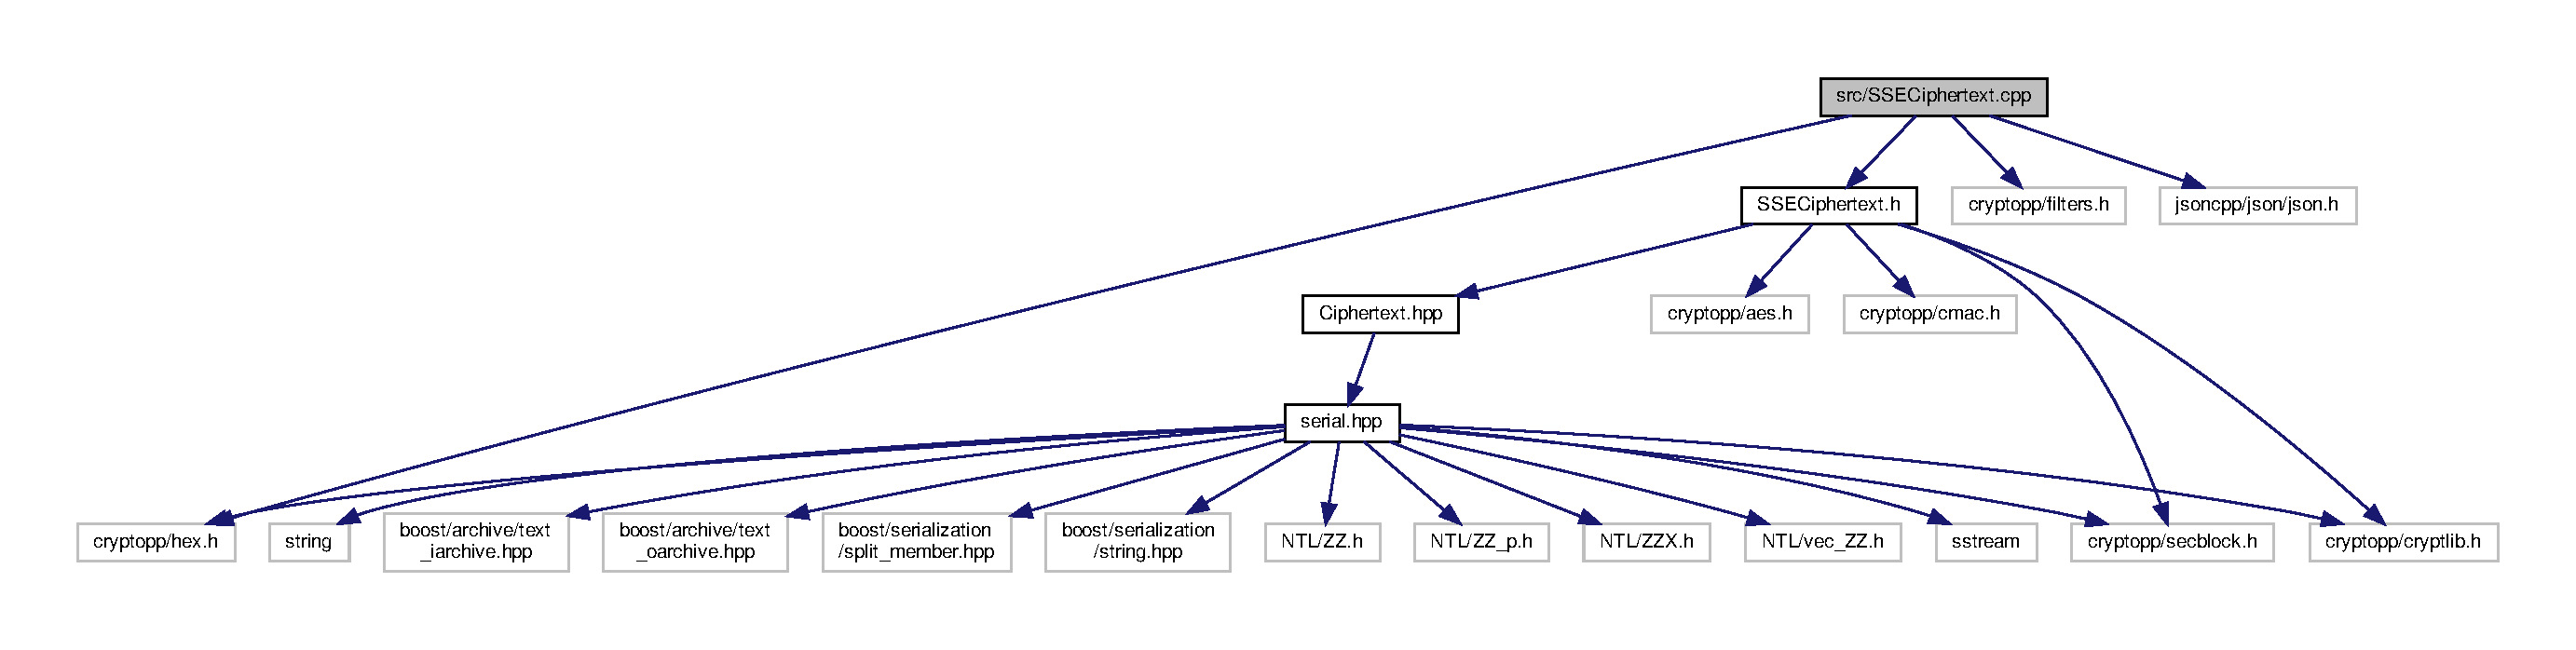
\includegraphics[width=350pt]{SSECiphertext_8cpp__incl}
\end{center}
\end{figure}

%--- End generated contents ---

% Index
\backmatter
\newpage
\phantomsection
\clearemptydoublepage
\addcontentsline{toc}{chapter}{Index}
\printindex

\end{document}
